%%%%%%%%%%%%%%%%%%%%%%%%%%%%%%%%%%%%%%%%%%%%%%%%%%%%%%%%%%%%%%%%%
%                          Packages                             %
%%%%%%%%%%%%%%%%%%%%%%%%%%%%%%%%%%%%%%%%%%%%%%%%%%%%%%%%%%%%%%%%%
\documentclass[a4paper,11pt]{report}
\usepackage[utf8]{inputenc}
\usepackage[a4paper, top=3cm, bottom=3cm, left=2.5cm, right=2.5cm, marginparwidth=2cm, headsep=1.2cm]{geometry} % layout
\usepackage[pdfencoding=auto]{hyperref} % enables hyperlinks in the PDF
\hypersetup{colorlinks=true, linkcolor=black, urlcolor=blue, citecolor=black} \urlstyle{same}
\usepackage{amsmath}
\usepackage{longtable}
\usepackage{cleveref} \Crefformat{figure}{#2Fig.~#1#3} % makes referencing customizable (e.g. \Cref{}). See: https://texblog.org/2013/05/06/cleveref-a-clever-way-to-reference-in-latex/)
\usepackage[nottoc, notlof, notlot]{tocbibind}  % includes bibliography in table of contents (TOC)
\usepackage[numbers]{natbib} % sets reference style
\usepackage{graphicx} % required to include images
\usepackage[svgnames]{xcolor}
\usepackage{tikz}

\usepackage{pgfplots}
\pgfplotsset{compat=1.17}

\usepackage{subfig}
\usepackage{siunitx} % makes it easier to use units (e.g. \SI{15}{mm}). See: https://mirror.foobar.to/CTAN/macros/latex/contrib/siunitx/siunitx.pdf
\usepackage[font=small]{caption} % reduces the caption's font size
\usepackage{eso-pic} % required to add the titlepage background image
\usepackage{lipsum} % To generate lorem ipsum dummy text
\usepackage{pgfgantt} % For Gantt chart creation
\usepackage{fancyhdr} % Changes the header & footer style
\usepackage{float}
\usepackage{bm}
\usepackage{amsfonts} 
\usepackage{booktabs}
\usepackage{multirow}
\usepackage{listings}
\usepackage{listings-golang}
\usepackage{adjustbox}
\usepackage{multicol}

\lstset{
  language=golang,
  showstringspaces=false,
  columns=flexible,
  basicstyle={\small\ttfamily},
  numbers=none,
  numberstyle=\tiny\color{mygray},
  keywordstyle=\color{blue},
  commentstyle=\color{mygreen},
  stringstyle=\color{mymauve},
  breakatwhitespace=true,
  tabsize=4
}

\usepackage[ruled,vlined,linesnumbered]{algorithm2e}

\usepackage{placeins}
\usepackage{enumitem} % for enumerated lists other than 1. 2. 3. 
\usepackage{algpseudocode}

%%%%%%%%%%%%%%%%%%%%%%%%%%%%%%%%%%%%%%%%%%%%%%%%%%%%%%%%%%%%%%%%%
%                          Commands                             %
%%%%%%%%%%%%%%%%%%%%%%%%%%%%%%%%%%%%%%%%%%%%%%%%%%%%%%%%%%%%%%%%%
% Author
% Use \\ to separate multiple authors (e.g. Robert\\Nathalie\\Mike)
\newcommand{\myName}{SOMAS Class 2021--2022}

% Title
% Introduce line breaks with \\
\newcommand{\myTitle}{Self-Organising Multi-Agent Systems}

% Type of Thesis
\newcommand{\thesisType}{Final Report}

% Date
\newcommand{\myDate}{January 2022}

% Supervisors
% Use \\ to separate multiple supervisors (e.g. Robert\\Nathalie\\Mike)
% Use full titles (e.g. Prof. Dr., Dr. )
\newcommand{\supervisors}{Prof.\ Jeremy Pitt}

% ToDo Command
\newcommand{\ToDo}[1]{\textcolor{red}{#1}}

%%%%%%%%%%%%%%%%%%%%%%%%%%%%%%%%%%%%%%%%%%%%%%%%%%%%%%%%%%%%%%%%%
%                          Page Format                          %
%%%%%%%%%%%%%%%%%%%%%%%%%%%%%%%%%%%%%%%%%%%%%%%%%%%%%%%%%%%%%%%%%

% Paragraphs
\setlength\parindent{0pt}
\setlength{\parskip}{2mm}

% Section Format
\usepackage[explicit]{titlesec}

%%%%%%%%%%%%%%%%%%%%%%%%%%%%%%%%%%%%%%%%%%%%%%%%%%%%%%%%%%%%%%%%%
%                        Title Page                             %
%%%%%%%%%%%%%%%%%%%%%%%%%%%%%%%%%%%%%%%%%%%%%%%%%%%%%%%%%%%%%%%%%
% Don't change anything here
\begin{document}
\begin{titlepage}
\newgeometry{top=2cm, bottom=4cm, right=1.5cm, left=1cm}

\tikz[remember picture,overlay] \node[opacity=1,inner sep=0pt, anchor=west] (A) at (2cm,-1.5cm){
\includegraphics[scale=0.5]{template_figures/logo.eps}};

    \begin{center}
        \vspace*{6cm}
        \huge \textbf{\thesisType}\\
        \vspace*{0.75cm}
        \Huge \myTitle\\
        \vspace{0.5cm}
        \Large {Department of Electrical and Electronic Engineering}\\
        \Large {Imperial College London}\\
        \vspace*{5cm}
        \huge \myName\\
        \vspace*{0.5cm}
        \LARGE \myDate\\
        \vfill
        Lecturer\\
        \vspace*{0.5cm}
        \huge \supervisors\end{center}

\end{titlepage}

%%%%%%%%%%%%%%%%%%%%%%%%%%%%%%%%%%%%%%%%%%%%%%%%%%%%%%%%%%%%%%%%%
%               Abstract & Table of Contents                    %
%%%%%%%%%%%%%%%%%%%%%%%%%%%%%%%%%%%%%%%%%%%%%%%%%%%%%%%%%%%%%%%%%
\pagenumbering{roman}

\begin{abstract}
Co-operative survival games refer to a subset of political choice games wherein `players' must work together to overcome disaster, else suffer the consequences through both personal and communal damage. Furthermore, without the ability to monitor a system and in the absence of a centralised authority, it becomes impossible to form enduring self-governing institutions, resulting in the proposed self-organising mechanisms for `solving' such games potentially functioning in harmful ways. This project utilises a self-organising, multi-agent system to simulate an iterated collective action, co-operative survival game comprising a resource management problem, the `solution' to which involves a system of localised governance. Through a series of experiments where the behaviour of the players in the system is increasingly randomised and the presence of self-organising mechanisms is toggled, we investigate the causes of instability. Ultimately, we conclude that through the integration of governance using treaties, it is possible for such a system to effectively self-organise to minimise the total deaths of the players involved.
\end{abstract}

\newpage
\tableofcontents
\newpage

\pagenumbering{arabic}

%%%%%%%%%%%%%%%%%%%%%%%%%%%%%%%%%%%%%%%%%%%%%%%%%%%%%%%%%%%%%%%%%
%                      Document Start                           %
%%%%%%%%%%%%%%%%%%%%%%%%%%%%%%%%%%%%%%%%%%%%%%%%%%%%%%%%%%%%%%%%%

\chapter{Introduction}\label{introduction}

\section{Problem Statement}
Section on the tower and how we have interpreted the spec.
Should include a basic spec for features that we wanted to achieve

\section{Our Goals}
Getting a simulation environment working
\chapter{Simulation Structure}\label{simulation_structure}
%%%%%%%%
%%%%%%%% Scenario and Simulator
%%%%%%%%
\section{Scenario and Simulator}\label{scenario_and_simulator}

\subsection{Context}

The Platform presents an environment consisting of people subjected to a life within a tower. This tower has a predefined set of laws that closely control the people’s lives, and it is ultimately up to these individuals to act however they suppose is correct.
 
The tower is made up of multiple floors with one agent per floor, starting with Floor 1 at the top and increasing downwards. Above Floor 1, there is a kitchen which produces a fixed amount of food per day.
The floor on which people are based is random, and periodically reshuffles with a fixed frequency. At the beginning of each day a platform begins moving down the tower, starting from the top floor where it is loaded with food and stopping for a constant time at each floor. Over a period of time, there is enough food on the platform to minimally satisfice the agents, but not maximally satisfy them all.
 
The people exist with limited knowledge of tower; they must eat enough within a period to survive and can communicate with other individuals on local floors. They know which floor they are on, but do not know how many floors there are in the tower nor how much food there is at the beginning of each day. Additionally, the people in the tower do not explicitly know how often the reshuffle period is. Finally, when a person dies, they are immediately replaced.

The scenario presented above is heavily influenced by \textit{`El Hoyo'}\citep{elhoyo2019} (translating directly to `The Hole') a Spanish film released in 2019.

\subsection{Assumptions}


There are several assumptions from the given context and, for the implementation in this project, are described in this section.

\begin{enumerate}
    \item  Pre-existing knowledge -- people exist in the tower with a level of knowledge of their environment; this reduces the amount of learning required before action can take place. Pre-existing ideologies are included in this: people have their ways of interacting with others, views on socialising and the like, perhaps acquired from a life before the tower.
     Basic concepts such as consuming food to increase health are known.
      \item  Taking food -- people are allowed to take as much food from the platform as they are able to eat. They cannot preserve food to eat on separate days. Additionally, the utility of the food taken decreases exponentially (each unit of food has a decreasing improvement to HP) -- representing the law of diminishing returns.
      \item An honest environment -- people are assumed to be truthful: direct deceit does not exist. There are very specific conditions in which deceit is permitted, these will be discussed alongside the introduction of the relevant features, but is related to breaking agreements in times of extreme need.

\end{enumerate}

\subsection{Observations \& Understanding}

An initial observation of the context immediately presents the concept of a `world', i.e., the tower, and `agents', i.e.,  the people. These agents interact with one another and the tower, within constraints, and must be able to react and evolve their behaviour to maximise their utility and survival.
 
 
Within the tower there exists a food allocation problem, which is directly related to the survival of agents and forms the core incentive for self-organisation. With a lack of organisation, the tower society would fall victim to the tragedy of the commons -- the common pool resource would deplete, and the overall well-being of society would suffer for the gain of a few individuals. Hence, the crux of this project is a collective action resource management problem, and agents must be equipped with sufficient capabilities and information.
 
The aforementioned capabilities can be split into two sections: those related to the tower and those related to the agent interactions.
 
Within the tower, agent abilities are listed below:
\begin{enumerate}
    \item View Food on Platform -- the agent cannot view the amount of food on the platform unless it is on the agent’s floor or the floor immediately below the agent.
    \item Food Consumption -- agents cannot preserve food. Agents can only eat food from the platform when it is on the agent's floor.
    \item Time Details -- agents do not have explicit access to timed parameters (reshuffle period, day length, time of platform on each floor etc.), however, can use memory to calculate these.
    \item Food Details -- agents do not know the food on the platform at the beginning of each day.

    \item Health Details -- agents do know their current health level and the utility they are receiving from food, as well as how long they can go without food before dying.
    
\end{enumerate}

Agents are also able to communicate with each other:
\begin{enumerate}
    \item Agents should be able to converse with one another and share information.
    \item Agents should be able to form agreements which must be followed.
    \item Agents should be able to differentiate between any new agents that appear locally.
    \item The communication must be limited to single agent interactions and single messages cannot travel past a defined, local distance. 
\end{enumerate}

%%%%%%%%
%%%%%%%%System Design
%%%%%%%%
\section{System Design}\label{system_design}

Based on our initial observations and constraints, possible implementations were explored early on in the design process. Our design process evolved from designing for the simple use case of allowing simple agents to eat food and communicate with primitive messages, to scaling this up to accommodate multiple agents on multiple floors.

\subsection{Ticks and Timing Details}

Discrete time in the simulation is represented by ticks. During each tick, all agents can perform an action such as `eat' or `send a message'. This means that the number of ticks per day restricts the communication between the agents. Moreover, given that messages can only be passed from one floor to one below or above on each tick, we can conclude that certain messages will never get to their receiver. The number of ticks per day is set in the initialisation of the simulation and is the product of the ticks per floor and the number of floors.

\subsection{Agent Configuration}

Agent structures are separated into two different aspects: a base agent and a custom agent, both of which are required to represent a single agent.
The base agent component contains the core information of an agent, including its Health Points, Floor and UUID\footnote{UUID -- Universally Unique Identifier}, as well as a pointer to the tower structure. 
The custom agent contains a pointer to its base agent and any parameters relevant to the specific agent behaviour; this varies between agent types and was implemented by agent teams.

The core parameters of an agent were abstracted out of the custom agent for two reasons:
\begin{enumerate}
    \item Custom agents cannot manipulate their own data or information, rather they can only request access through `getter' functions, which returns either information or an error.
    \item The tower struct has access to the base agents and can therefore influence the agent parameters as determined by the laws existing within the tower. Examples of this include floor reshuffling and health decay.
\end{enumerate}

\subsection{Death and Replacement}

Deaths occur in the tower when an agent has not eaten enough food to stay alive over a certain duration. The nature of replacement in the tower could be of several types:
\begin{enumerate}
    \item Replacing agents with random agent type
    \item Replacing agents with the same agent type
    \item Replacing agents with the dominant agent type
\end{enumerate}

Our design chose to replace agents with the same agent type. While replacing agents with a random agent type would introduce an element of uncertainty, this would have made it difficult to analyse individual agent behaviours. It would have been interesting to experiment with replacing agents with the dominant agent type, however, this posed the question of defining what the most ``dominant'' agent would be.

\subsection{Infrastructure}

Our implementation began with considering the structure of the system given the scenario we had identified. The key required components include a tower that contains agents, with a discrete-time system.
The simulation package holds the state of the tower, base agents, and their corresponding custom agents. The simulation package that creates the world and constructs agents inside a simulation environment. It is the simulation that calls the tower and agent functions to progress the simulation.
The tower is the overall `world' which stores information in its state such as the list of agents, platform level, food available, and tick count. The tower is responsible for updating the platform, reshuffling agents, and replacing dead agents.
The platform is a parameter of the tower and stores the amount of food on the platform and its current floor. It goes down one floor at a predefined tick rate (e.g., every 10 ticks) and it is reset (fill the platform with food and set its floor to 1) at the end of each day.

Base agent contains the core information of an agent, such as an agent's HP and floor. Base agent also contains the \lstinline$hpDecay()$ function as well as a function to calculate an individual agent's utility. 
Custom agents are designed by each of the agent teams, where each one of them has a different strategy.

%%%%%%%%
%%%%%%%% Message Passing
%%%%%%%%
\section{Message Passing}\label{message_passing}
\subsection{Primitive Messaging}
An important role of Team 1 was to design a mechanism for agents to talk amongst each other in the simulation that would allow automated communication. The first step in this process was to design a system which would allow an agent to pass along a minimum viable message to their neighbours. These were the goals of communication in the MVP:
\begin{itemize}
    \item Agents could only talk to their immediate neighbors ($\pm1$ floor).
    \item Agents should be given the ability to ignore communication.
    \item Multiple agents could be ``speaking'' in a given tick.
    \item One agent can send one message per tick.
    \item \textbf{It is entirely at an agent's discretion if/when/how they wish to react to a message as long as their behavior is not deceptive}
\end{itemize}

As a team, Team 1 emphasized the last point. The infrastructure should not force any behavior onto the agent as long as the behavior was honest. The basic philosophy of the communication infrastructure was to dictate as little as possible about the agent's behavior while keeping the API readable and user-friendly. This meant providing basic override-able behaviors that were as unobtrusive as possible to team strategies. \newline
The infrastructure should not force any behaviour onto an agent as long as the behaviour is honest. The basic philosophy of the communication infrastructure was to dictate as little as possible about the agent's behaviour while keeping the API readable and user-friendly. This usually meant providing basic override-able behaviours to be as unobtrusive as possible to team strategies. \newline
\begin{itemize}
    \item \textbf{\texttt{MessageType}}: Indicates one of 13 enumerated message types.
    \item \textbf{\texttt{SenderFloor}}: Returns the floor this message was sent from.
    \item \textbf{\texttt{TargetFloor}}: Returns the floor the message is addressed to.
    \item \textbf{\texttt{ID}}: Each message sent is given a unique ID.
\end{itemize}
\vspace{\baselineskip}
For the MVP, Team 1 constructed a system in which, for example, when Alice (currently at floor 30) wishes to send a message upward:
\begin{enumerate}
    \item At Tick 0, Alice would construct the message for Bob containing the following information:
        \begin{itemize}
            \item \textbf{Alice's ID}
            \item \textbf{Alice's current floor}: 30
            \item \textbf{Message's target floor}: 29 \textit{Since Alice wants to message the floor above her}
            \item \textbf{Message Type} (to be elaborated on the Common Languages Section)
        \end{itemize}
    \item Still at Tick 0, Alice calls \texttt{SendMessage} which takes her message and passes it to the tower.
    \item The tower acts as the communication authority, finding the agent who is on floor 29 at Tick 0 and inserting the message into the recipient agent's (Bob's) inbox.
    \item At Tick 1, Bob may choose to call \texttt{ReceiveMessage} which would extract Alice's message (if Alice was the first or only agent to send him a message at Tick 0) and respond.
    \item If Bob has called \texttt{ReceiveMessage}, Alice's message is removed from Bob's inbox.
\end{enumerate}
With this implementation, each agent is responsible for calling \texttt{ReceiveMessage} once per tick to receive any messages. The inbox is a FIFO queue -- if multiple messages are received or if there are outstanding messages from previous ticks, only the earliest one can be retrieved in a given tick.
Additionally, ``receiving" does not necessarily imply ``reacting". An agent is capable of receiving a message and not responding to it at all without the sender's knowledge. Decoupling ``receiving" and ``reacting" gave agent teams the freedom to ignore messages entirely (metaphorically covering their ears in the tower and refusing to listen to anybody), to listen to messages and do nothing about them, or to actively listen and react. \newline
Beyond the MVP, however, messages needed to have meaning. Because the process would be automated it was meaningless to send unstructured strings, how was an agent to understand ``Please only eat what you need to survive."? \newline
A common language was necessary.

\subsection{Common Language}
To design the common language, Team 1 surveyed the agent teams asking for what they would like to talk to other agents about. We collected suggestions and found that communication indicated one of four possibilities:
\begin{enumerate}
    \item An agent could be \textit{asking} another agent for information. ``How much food is on the platform when it gets to you?" or ``How much food did you take?"
    \item An agent could be \textit{stating} something about its state or environment. ``I am in critical (health) condition" or ``There is no more food left on the platform"
    \item An agent could be \textit{request} something from another agent. ``Please leave 10 food on the platform for me."
    \item An agent could be \textit{responding} to another agent's request. ``Yes." or ``No."
\end{enumerate}
These categories solidified into four basic messages - \texttt{Ask}, \texttt{State}, \texttt{Request}, and \texttt{Response}. \newline
In addition, \texttt{Ask} and \texttt{Request} are messages that expect a response. A \texttt{State} message could be a response to an \texttt{Ask} but also could be an unprompted announcement while \texttt{Response} must be responding to some pre-existing \texttt{Request}. \newline 
While Team 1 did not want to force agent teams into any behaviors, we wanted to make the API compatible with the expected etiquette of communication. This lead to the message categorization and pair-wise reply functionality summarized below.
\begin{center}
\begin{tabular}{p{3cm}p{3cm}p{5cm}p{3.5cm}}
 \hline
 \textbf{Message \newline Category} & \textbf{Reply \newline Category} & \textbf{Body Functions} & \textbf{Description} \\ [0.5ex] 
 \hline\hline
 \texttt{AskMessage} & \texttt{StateMessage} &  \texttt{Reply}: Returns appropriate statement & Inquires something about a neighboring agent's state. \\
 \hline
 \texttt{StateMessage} & N/A & \texttt{Statement}: Returns the value of statement. \textit{e.g. a StateHP message of 5HP would return 5.} & Announces something about an agent's state or environment. \\ 
 \hline
 \texttt{RequestMessage} & \texttt{ResponseMessage} & \texttt{Reply}: Returns \texttt{BoolResponse} \newline \texttt{Request}: Returns the value of a request \textit{e.g. a RequestLeaveFood message that requests an agent to leave 10 food would return 10 on \texttt{Request}} & Asks how much food is on the platform when it arrives at the (recipient) agent \\ 
 \hline
 \texttt{ResponseMessage} & N/A & N/A & Asks how much food an agent is planning to take \\ 
 \hline
\end{tabular}
\end{center}
From these basic categories 11 specific messages were developed that specified what was being asked, stated, requested or responded to.
\begin{center}
\begin{longtable}{p{4cm}p{2.5cm}p{4cm}p{4cm}}
 \hline
 \textbf{Message Type} & \textbf{Category} & \textbf{Description} & \textbf{Reply Type} \\ [0.5ex] 
 \hline\hline
 \texttt{AskFoodTaken} & \texttt{AskMessage} & Asks how much food an agent has (already) taken
 & \texttt{StateFoodTaken} \\ 
 \hline
 \texttt{AskHP} & \texttt{AskMessage} & Asks how much HP an agent has & \texttt{StateHP} \\ 
  \hline
 \texttt{AskFoodOnPlatform} & \texttt{AskMessage} & Asks how much food is on the platform when it arrives at the (recipient) agent & \texttt{StateFoodOnPlatform} \\ 
 \hline
 \texttt{AskIntendedFoodIntake} & \texttt{AskMessage} & Asks how much food an agent is planning to take & \texttt{StateIntendedFoodIntake} \\ 
 \hline
 \texttt{StateFoodTaken} & \texttt{StateMessage} & States how much food an agent has taken &   \\
 \hline
 \texttt{StateHP} & \texttt{StateMessage} & States how much HP an agent has &   \\
 \hline
 \texttt{StateFoodOnPlatform} & \texttt{StateMessage} & States how food is on the platform when it arrives to the agent &  
 \\
 \hline
 \texttt{StateIntendedFoodIntake} & \texttt{StateMessage} & States how food the agent is planning to take &  
 \\
 \hline
 \texttt{RequestLeaveFood} & \texttt{RequestMessage} & Requests that an agent (presumably above) you leaves a certain amount of food on the platform & \texttt{BoolResponse}
 \\
 \hline
 \texttt{RequestTakeFood} & \texttt{RequestMessage} & Requests that an agent (presumably above) you takes a certain amount of food on the platform & \texttt{BoolResponse}
 \\
 \hline
 \texttt{BoolResponse} & \texttt{ResponseMessage} & Message affirming or rejecting a request &  
\end{longtable}
\end{center}
The distinction between ``receiving" and ``reacting" becomes important. Because we wanted to ensure that \textit{receiving} any of these message types did not mean that the recipient had to \textit{react}, the ``reaction" was separated into an external function which the agent could optionally call after they extracted their message from the inbox. \newline
The design works such that if Alice on Floor 11 wanted to ask Floor 12 to leave 10 food on the platform for her:
\begin{enumerate}
    \item At Tick 0, Alice constructs a \texttt{RequestLeaveFoodMessage} with \texttt{Request} set to 10 addressed to Floor 12.
    \item At Tick 0, Alice sends the message.
    \item At Tick 1, Bob (whose inbox was previously empty and who was listening for messages) receives Alice's message. If he chooses to react, he decides whether or not he wants to cooperate with Alice and generates his response with the \texttt{Reply} function of the message (no need to construct the \textit{BoolResponseMessage} himself).
    \item At Tick 1, he sends his reply back, addressed to the message's sender floor.
    \item At Tick 2, Alice (whose inbox was also previously empty) receives Bob's response and may choose to react to it.
\end{enumerate}
The system so far provided a solid mechanism for agents to communicate to their neighbours, to gather information and to request help in times of crisis (potentially building trust or temporary relationships). However, it was contingent on communicating agents being on consecutive floors, any relationships built through this kind of communication could only last for a reshuffle period unless the agent implemented a specific kind of internal memory structure. Additionally, the communication was still relatively rudimentary. Alice's request for 10 food could be rejected by Bob because his HP is critical and he will starve immediately without food, but the current system only allows Bob to either accept or refuse Alice's request without communicating anything about his own state. This could potentially worsen his relationship with Alice, had Alice known that Bob was in a critical state perhaps her trust to him would not degrade because of this rejection. \newline 
For more nuanced, long-lasting communication, treaties and message propagation were needed.

\subsection{Treaties}
Treaties are formalized agreements between agents who agreed to a set of conditions and corresponding requests. An example treaty might be \textit{“Please leave 40 food on the platform if you are not in critical condition”}. In an honest run of the experiment deception was disallowed and it was ensured that if an agent agreed to a treaty, they would be be bound to uphold it. \newline
This required designing an internal mini-language for how treaties should be written and understood. It was decided that a treaty consisted of 6 language components:
\begin{center}
\begin{tabular}{p{4cm}p{11.5cm}}
 \hline
 \textbf{Field} & \textbf{Description} \\ [0.5ex] 
 \hline\hline
 \texttt{ConditionType} & 
 Dictates the type of condition the treaty is active with possibilities of:
 \begin{itemize}
    \item \textbf{\texttt{HP}}: The treaty's activeness is dependent on the signing agent's HP.
    \item \textbf{\texttt{Floor}}: The treaty's activeness is dependent on the signing agent's current floor.
    \item \textbf{\texttt{AvailableFood}}: The treaty's activeness is dependent on the signing agent's available food (food on platform).
\end{itemize} \\
 \hline
 \texttt{ConditionOp} & Includes all the mathematical operators $\geq, >, =, <, \leq$ \\ 
 \hline
 \texttt{ConditionValue} & Value that the \texttt{ConditionType} has to meet the \texttt{ConditionOp} for. \\ 
 \hline
 \texttt{RequestType} & The request agreement for the treaty, possible requests are:
 \begin{itemize}
    \item \textbf{\texttt{LeaveAmountFood}}: Requests a signed agent to leave a fixed amount of food.
    \item \textbf{\texttt{LeavePercentFood}}: Requests a signed agent to leave a percentage of food on the platform.
    \item \textbf{\texttt{Inform}}: Requests a signed agent to alert their neighbor if treaty conditions are met.
\end{itemize} \\ 
 \hline
 \texttt{RequestOp} & Includes all the mathematical operators $\geq, >, =, <, \leq$ \\ 
 \hline
 \texttt{RequestValue} & Value that the \texttt{RequestType} has to meet the \texttt{RequestOp} for. \\ 
 \hline
\end{tabular}
\end{center}
\vspace{\baselineskip}
The aforementioned treaty \textit{“Please leave 40 food on the platform if you are not in critical condition”} would be translated into \newline
\texttt{ConditionType = HP \newline
        ConditionOp = GT \newline
        ConditionValue = 20 //(where 20 is the critical threshold) \newline
        RequestType = LeaveAmountFood \newline
        RequestOp = EQ \newline
        RequestValue = 40 \newline}
In addition to the language components the treaties included a \texttt{SignatureCount} which tracked an estimate of how many agents had signed the treaty thus far. This number was not an accurate, it only vaguely indicates whether or not a treaty is popular. 
The introduction of treaties also necessitated the creation of one more message category as well as a message sub-type. 
\begin{center}
\begin{tabular}{p{3cm}p{3cm}p{5cm}p{3.5cm}}
 \hline
 \textbf{Message \newline Category} & \textbf{Reply \newline Category} & \textbf{Body Functions} & \textbf{Description} \\ [0.5ex] 
 \hline\hline
 \texttt{ProposalMessage} & \texttt{ResponseMessage} &  
 \texttt{Reply}: Returns \texttt{TreatyResponseMessage} \newline 
 \texttt{Treaty}: Returns the treaty that the proposal is carrying &
 Carries a treaty from proposer/propagator to recipient.\\
 \hline
\end{tabular}
\end{center}
\texttt{TreatyResponse} sub-type of \texttt{ResponseMessage} which were response messages that contained the ID of the treaty it was responding to. \newline
The treaties-relay-design and the inaccuracy of the signature count is illustrated if Alice, still on Floor 10, wanted to propose the treaty \textit{“Please leave 40 food on the platform if you are not in critical condition”} to her neighbours downstairs and upstairs it would work as follows:
\begin{enumerate}
    \item Tick 0: Alice constructs the treaty, embeds it within a \texttt{ProposeTreatyMessage} and sends it upward (as she can only send one message per tick). Alice's treaty begins with a \texttt{SignatureCount} of 1 (since she implicitly signed it by proposing).
    \item Tick 1: Treaty arrives on the 11th Floor in Bob's (previously empty) inbox and he chooses to respond positively and signs. On Bob's local copy of the treaty, the \texttt{SignatureCount} has incremented to 2 but not on Alice's. Bob replies through \texttt{Reply} and sends the  \texttt{TreatyResponse} downstairs.
    \item Tick 1: Meanwhile, Alice also sends the treaty downward to Floor 9.
    \item Tick 2: Treaty arrives on the 9th Floor in Carol's (previously empty) inbox and she also chooses to respond positively. \newline
    Here, Carol's local copy of the treaty has a \texttt{SignatureCount} of 2 not 3 despite the fact she is the third person to sign.
    \item Tick 2: Meanwhile, Alice has received Bob's affirmation. Knowing that he signed it, she increments her copy of the treaty.
    \item Tick 3: Alice also receives Carol's affirmation, she increments her local \texttt{SignatureCount} to 4, making her the only person with access to the correct signature numbers.
    \item Tick \texttt{n}: In some future tick post-reshuffle where Alice, Bob and Carol are no longer neighbours, the three of them and whoever else signed copies of the treaty (if Carol or Bob further propogated the treaty) are bound to the agreement that if they are not in critical condition, they would leave 40 food)
\end{enumerate}
Although we discussed several approaches for keeping an accurate state of the \texttt{SignatureCount}, they required too much communication overhead which could be detrimental to strategies since messages were capped at one per tick. Agent teams opposed the idea of removing the field altogether so an inaccurate but potentially useful \texttt{SignatureCount} was kept. \newline
Because the honest run of the experiment required that no agent would break their treaties, by default agents would reject treaties. This default was expected to be overridden by any agent team who wanted to communicate with other agents so this introduced difficulties in how to ensure that treaties that had been signed were followed. There were suggestions for a technical solution however ultimately that was too restrictive for agent strategies as it would require Team 1 to somehow conditionally override agent behavior depending on if they had an active treaty or not which was technically difficult but also extremely limiting for the agents. Ultimately it was decided that the honesty would be maintained through thorough a combination of readable agent code and thorough PR (pull request) reviews from Team 1 as treaty-strategies were implemented. \newline
With the advent of treaties and the possibility of building relationships that outlived a reshuffle, it was time to extend communications beyond immediate neighbors to possibly tower-wide.

\subsection{Message Propagation}
Multi-floor communication was a long-awaited feature among agent teams so there had already been many conversations about how best to achieve this. There were two main approaches.
\begin{enumerate}
    \item \textbf{Shouting}: An agent could shout up or down a specified number of floors and every agent the in-between floors could also hear.
    \item \textbf{Directed Shouting}: An agent could shout in such a way that only the agent on the targeted floor would hear but none of the agents in the in-between floors could.
    \item \textbf{Propagating}: An agent could only speak to its immediate neighbour but they could instruct their neighbour to pass the message on to the target floor.
\end{enumerate}
Option 2 was eliminated quickly for its unreasonable premise, it was not clear conceptually how an agent could yell only to one recipient. \newline
Option 1 required some limit on the number of floors you could yell across. Agent teams also suggested that shouting should not be a free action and should ``cost" HP when engaged in often. Although interesting, it introduced unnecessary complexity and was eliminated. \newline
Option 3 also had some interesting implications. There were multiple possibilities in how the in-between agents would behave:
\begin{itemize}
    \item An in-between agent could break the propagation chain and not inform the original sender.
    \item An in-between agent could tamper with the message before passing it on.
    \item An in-between agent could eavesdrop on the message being passed.
\end{itemize}
After some discussion, it was decided that for honest experiments breaking the chain without informing and message-tampering were disallowed while eavesdropping remained legal. \newline
We set the default behavior of propagation to be ``dutifully pass the message if it was not addressed to your floor" on the infrastructure level. This was so agents who did not wish to eavesdrop or did not engage in intra-agent communication at all would not need to implement separate handlers for propagation. \newline
With the completion of message propagation, communication mechanisms within the tower were finished.

%%%%%%%%
%%%%%%%% Health Modeling
%%%%%%%%
\section{Health Modeling}\label{health_modeling}

%
%%%%%%%% Global Description
%
\subsection{Global Description}

The health of the agents living in the tower is represented by Health Points (HP). Two mechanisms affect an agent's HP: how much food they eat, and their ``cost of living''. The cost of living represents how many calories a human needs to eat each day to stay healthy. These two mechanisms are implemented using the functions \lstinline$updateHP$ and \lstinline$hpDecay$, respectively. These two functions are described below.

At the end of each day, agents are assigned an HP value based on how much food they have eaten and their cost of living. This HP value is an integer and has a maximum value of \lstinline$MaxHP$, and a minimum value of \lstinline$HPCritical$. As its name suggests, \lstinline$HPCritical$ is a critical HP value for the agents: they can only survive a certain number of days (\lstinline$MaxDayCritical$) at this level. When in the critical state, if agents can increase their HP by \lstinline$HPReqCToW$ (``HP Required to move from Critical To Weak''), then they move into the \lstinline$WeakLevel$ (\Cref{fig:health_system}), and their HP takes the value of \lstinline$WeakLevel$. The amount that an agent's HP increases from eating is determined by the function \lstinline$updateHP()$.

\begin{figure}[htb]
    \centering
    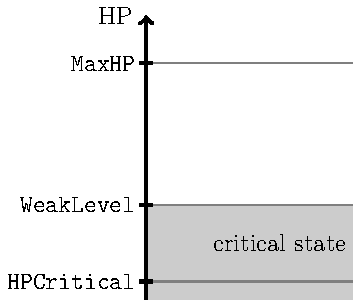
\includegraphics[width=0.3\linewidth]{002_simulation_structure/images/health_global.pdf}
    \caption{The health of the agents is represented by a HP value between \lstinline$HPCritical$ and \lstinline$MaxHP$. All HP values which are below \lstinline$WeakLevel$ are classed as critical. The diagram is not drawn to scale.}
    \label{fig:health_system}
\end{figure}

\subsection{Food and Health: \texorpdfstring{\texttt{updateHP}}{updateHP}}\label{updateHP}
To increase their HP, agents need to eat. However, the amount an agent's HP improves can saturate in a single day; eating more than a certain amount will provide an agent with no extra benefit to their HP. Moreover, eating more food will lead to diminishing returns in terms of HP change. Mathematically, the ideas of diminishing returns and saturation are well captured by the step response of a 1st-order system \eqref{updateHP_general}:

\begin{equation}\label{updateHP_general}
   \texttt{newHP}= \texttt{currentHP} +\underbrace{w(1-e^{\frac{-\texttt{foodTaken}}{\tau}})}_{\texttt{HPChange}}
\end{equation}

The two parameters $w$ and $\tau$ are defined at the beginning of the simulation. The shape of this curve is given in \Cref{fig:updateHP} together with some important parameters.

\begin{figure}[htb]%
    \centering
    \subfloat[\centering Overview]{{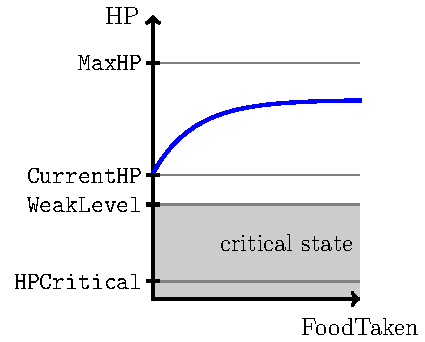
\includegraphics[width=0.36\linewidth]{002_simulation_structure/images/health_updateHP_overview.pdf}}}%
    \qquad
    \subfloat[\centering Detailed representation]{{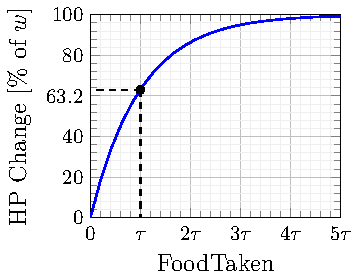
\includegraphics[width=0.36\linewidth]{002_simulation_structure/images/health_updateHP_detailed.pdf}}}%
    \caption{\texttt{updateHP} as a function of the amount of food eaten (``FoodTaken'').}%
    \label{fig:updateHP}%
\end{figure}

It is not possible to gain more HP than $w$ over the duration of one day; this is an intentional limit to prevent an agent's health from improving too quickly. As an example, we can think of an agent that starts from the weak level and wants to reach the maximum HP value. It would take several days for this agent to ``recover'' from this weak level and stabilise its health to a high HP value. 

Note that it is possible for an agent to achieve an HP value that is larger than \texttt{MaxHP} inside \lstinline$hpDecay$. At the end of each day, the \lstinline$hpDecay$ function will apply the cost of living and then bound the final HP value by \lstinline$MaxHP$.


Agents in the critical state are treated differently. For these agents, HP is updated according to equation \eqref{updateHP_critical}:

\begin{equation}\label{updateHP_critical}
    \texttt{newHP} = \min\left\{\texttt{HPCritical}+\texttt{HPReqCToW}, \texttt{currentHP} +w(1-e^{\frac{-\texttt{foodTaken}}{\tau}})\right\}
\end{equation}

\subsection{Cost of Living: \texorpdfstring{\texttt{hpDecay}}{hpDecay}}\label{hpDecay}
At the end of each day, the HP value of the agents will be reduced by the cost of living. The cost of living is larger for an agent with larger HP value than for an agent with lower HP value. This fact is motivated by a simple observation: humans that have stronger bodies and immune systems also need more food to sustain their level of health. The exact relation between HP value, cost of living, and HP value after applying the cost of living is given by the linear relation \eqref{hpDecay_equation}:

\begin{equation}\label{hpDecay_equation}
    \texttt{newHP} = \texttt{currentHP}-\left[b + s(\texttt{currentHP}-\texttt{WeakLevel})\right]
\end{equation}


The parameter $b$ is a (constant) base cost, and $s$ is the slope of the linear function. These parameters are initialised at the beginning of the simulation.

To ensure that the HP value at the end of the day is bounded by \texttt{MaxHP}, we slightly modify (\ref{hpDecay_equation}) to produce (\ref{hpDecay_bounded}):

\begin{equation}\label{hpDecay_bounded}
    \texttt{newHP} =\max\left\{\texttt{MaxHP}, \texttt{currentHP}-\left[b + s(\texttt{currentHP}-\texttt{WeakLevel})\right]\right\}
\end{equation}

For agents in the critical state that gain \texttt{HPReqCToW} HP in a single day, i.e. their HP after eating is

\begin{equation}\label{HPReqCToW}
    \texttt{currentHP} \geq \texttt{HPCritical}+\texttt{HPReqCToW},
\end{equation}

their HP will be set to \texttt{WeakLevel}. Agents in the critical state which do not manage to improve their HP by \lstinline$HPReqCToW$ will be kept in the critical state:

\begin{equation}\label{hpDecay_critical_stay}
    \texttt{newHP} = \texttt{HPCritical}
\end{equation}

with the \texttt{daysAtCritical} counter incremented by 1. If \texttt{daysAtCritical} reaches \texttt{MaxDayCritical}, the agent dies and is replaced. This counter is reset to 0 if an agent exits the critical state.




%%%%%%%%
%%%%%%%% Global Utility
%%%%%%%%
\section{Utility and Social Welfare}\label{utility}

To assess the performance of the agents in the tower as a group, we first need to define a metric. A common choice is the so-called \emph{social welfare}, based on each agent individual utility. For this project, we implement the notion of utility as introduced in \cite{somasPitt}.

Our system is composed of $N$ agents that can perform specific actions in relation with the common pool resources. In a general context, each agent 
$i\in\{1, \ldots, N\}$ takes the following actions at each iteration $t\in\{1,\ldots,\infty\}$:

\begin{enumerate}
    \item Determines the resources it has available, $g_i \in [0,1]$.
    \item Determines its need for resources, $q_i \in [0,1]$.
    \item Makes a provision of resources, $p_i \in [0,1]$.
    \item Makes a demand for resources, $d_i \in [0,1]$.
    \item Receives an allocation of resources, $r_i \in [0,1]$.
    \item Makes an appropriation of resources, $r'_i \in [0,1]$.
\end{enumerate}

In the current setup, the available resources $q_i$ corresponds to the current amount of food on the platform.  The need for resources $q_i$ is defined in relation with the health of the agents. We set the following values to $q_i$:

\begin{equation}\label{resources_needed}
    q_i=\begin{cases}
     \frac{\texttt{numberDaysInCriticalState}}{\texttt{maxDaysInCriticalState}} & \mbox{if } \texttt{currentHP}\leq \texttt{weakLevel}  \\ 
     0 & \mbox{else.}
     \end{cases}
\end{equation}

This way, we ensure that $q_i$ is bounded by 1 and is proportional to the days spent in the critical health zone below \texttt{weakLevel}.

Moreover, the agents do not make any provision $p_i$ to the common pool, as they cannot give food to the platform ($p_i=0$). Their demands for resources is the food they ask for when the platform is at their level. In addition, the agents appropriate all resources they are allocated, so that $r'_i=r_i$.\footnote{We ensure that all these parameters are constrained to the range $[0,1]$ by dividing the mentioned quantities by their maximum values.}

The total resources accrued at the end of an iteration, $R_i$, is hence defined as:

\begin{equation}\label{resources_accrued}
    R_i=r'_i+ (g_i-p_i)
\end{equation}

where each agent will `generate' resources equal to: its appropriation, plus the amount available on the platform, minus the provision made back to the common pool.

Using the above parameters, it is possible to compute the following utility per agent:

\begin{equation}\label{utility_per_agent}
    u_i=\begin{cases}
     \alpha_iq_i + \beta_i(R_i-q_i) & \mbox{if } R_i\geq q_i  \\ 
     \alpha_i R_i - \gamma_i(q_i-R_i) & \mbox{else}
     \end{cases}
\end{equation}


where $\alpha_i$, $\beta_i$ and $\gamma_i$ are tuning parameters that follow the rule $\alpha_i>\gamma_i>\beta_i$. In our work, we use the values $\alpha_i=\alpha=0.2$, $\beta_i=\beta=0.1$, and $\gamma_i=\gamma=0.18$.

Finally, we use \eqref{utility_per_agent} to compute an average global utility, which corresponds to the social welfare \textit{SW} divided by the number of agents:

\begin{equation}\label{utility_eq}
    \mathit{U}=\frac{\sum_i^N u_i}{N}=\frac{\mathit{SW}}{N}
\end{equation}

\section{Technology Stack}

Our technology stack was chosen in the initial meetings of the project, where the individuals were able to propose languages for the frontend and backend, with the backend language used to implement infrastructure and agents. The proposed languages for the backend were:
\begin{enumerate}
    \item Python: A widely used, general purpose programming language with an emphasis on code readability. The language was familiar to a large percentage of the class as a result of having used it in previous projects. 
    \item Go: A less well known language, Go was attractive to the class due to its easy-to-learn nature and easy implementation of concurrency which would be useful in running multiple agents. However, it was unfamiliar to the majority of the class.
    \item C++: A general purpose OOP language, C++ was familiar to a portion of the cohort having studied it in their first year. However, it is not as easy to learn as Go or Python, so this was considered a disadvantage.
\end{enumerate}

After an in-depth review, a vote was cast and Go was the clear preference. Overall, Go was chosen due to its advantages in implementing concurrency and its easy-to-learn nature. In addition to this, the packages in Go would make the code more scalable and readable.

React and Typescript were chosen as the frontend language. They were chosen primarily by the infrastructure team, as this decision would not affect those teams working on agent development. 

%%%%%%%%
%%%%%%%% Simulation Flow
%%%%%%%%
% \section{Simulation Flow}\label{simulation_flow}
% The order in which events happen
% Need a nice diagram for this


% %%%%%%%%
% %%%%%%%% Message Passing
% %%%%%%%%
% \section{Message Passing}\label{message_passing}
% Need a nice diagram for this
\chapter{Data Logging and Dashboard}\label{data_logging}

\section{Why do we need data?}

Data logging enables analysis of how internal variables change with time during a simulation. One might be interested in different variables from the system in question: messages frequency, food variation over time, agent deaths rate, etc... Analysis also requires linking different simulation parameters with the data logged (e.g. the number of agents or the amount of food available). 

It is therefore important to setup a logging framework that structures data effectively and scales efficiently for large simulations. The below subsections will introduce the simulation parametrisation, followed by the different logging strategies (dumps and structured), and concluding with the logging interface and the analysis dashboard.

\section{Parametrisation}

First, it was important to enable an effective parametrisation of the simulation. A configuration interface was therefore set to abstract variables from the simulation environment. A configuration object would therefore be passed to the simulation environment instance, and it would define the following simulation parameters:

\begin{multicols}{2}
    \begin{enumerate}
        \item Agent count for each team
        \item Agent count for random agents
        \item Agent count for selfish agents
        \item Agent HP
        \item Agents per floor
        \item Amount of food on the platform
        \item Food per agent ratio (optional)
        \item Ticks per floor
        \item Total days
        \item Reshuffle period
    \end{enumerate}
\end{multicols}

The configuration parameters could then be written in a simple \texttt{json} file which would be parsed into a configuration object.

\section{General log dumps}

Following the configuration work, a general logger was setup. The general logger is basically a single shared logger between the different instances in the system (simulation, tower, agents, etc...). Each instance appends by default an identifier to a log line in the general logger log file (named \texttt{main.json}). Here is an example below:

\begin{verbatim}
{"agent_id":"dece1252","agent_type":"Team5","floor":3,"health":100,
"level":"info","msg":"Reporting agent state of team 5 agent","reporter":"agent"}

{"Floor:":7,"HP:":100,"Social motive:":"Altruist","agent_id":"2bfd3cfb",
"agent_type":"Team6","level":"info","msg":"Reporting agent state:","reporter":"agent"}

{"agent_id":"7873bb50","agent_type":"Team1","floor":5,"health":100,
"level":"info","msg":"Reporting agent state","reporter":"agent"}
\end{verbatim}

The general log dumps are not structured yet they enable agent teams to directly log custom states from their agents and use those in e.g. evolutionary algorithms or machine learning training.

\section{Structured logs}

The general log generates huge amounts of data and therefore was ineffective for data analysis and drawing conclusions easily from different simulations. Therefore, structured logs had to be introduced, where particular data is captured optimally to generate lightweight, understandable logs. Following consultations with the agent teams and relating as fit to the problem, the following structured logs where included:

\begin{enumerate}
    \item \textbf{Food}: food available on the platform and food taken by agents.
    \item \textbf{Death}: agent death (including agent state at death time)
    \item \textbf{Messages}: receiver, sender, message type and content
    \item \textbf{Utility}: agent utility (including agent state)
    \item \textbf{Story}: a combination of the above logs in a sequential manner
\end{enumerate}

The agent state encapsulates by default the agent age, floor, HP, utility, and custom state (e.g. emotions or memory).

In the general log, custom agents could pass all sorts of information and therefore the log schema could not determined at compile time (which would be required for a visualisation dashboard). Structured logs have a well defined schema which does not depend on custom agents. For example, a food log will always have this form:

\begin{verbatim}
{"day":2,"food":19,"level":"info","tick":222,"time":"2022-01-17T02:13:37Z"}
{"day":2,"food":0,"level":"info","tick":262,"time":"2022-01-17T02:13:37Z"}
{"day":3,"food":100,"level":"info","tick":321,"time":"2022-01-17T02:13:37Z"}
{"day":3,"food":90,"level":"info","tick":322,"time":"2022-01-17T02:13:37Z"}
\end{verbatim}

With structured logs setup, it is now possible to bundle logging into an interface and connect it to a visualisation tool.

\section{Logging interface}

It was important to setup logging such as structured loggers could be easily extended with new loggers, while preserving the possibility to generate general logs. The following design has been adopted to encapsulate the simulation configuration and the loggers.

\begin{figure}[htb]
    \centering
    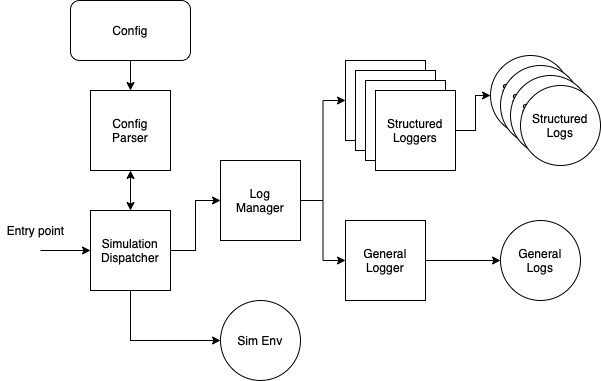
\includegraphics[width=0.8\linewidth]{003_data_logging/images/struct.png}
    \caption{Diagram showing how logging fits in the system}
    \label{fig:design_logging}
\end{figure}

The entry point to the simulation dispatcher was then linked to both the CLI as well as a server (with HTTP listeners) to support a browser-based dashboard.

\section{Dashboard}


\chapter{Team 2 Agent Design}\label{team_2_agent_design}

\SetKwComment{Comment}{$\triangleright$\ }{}

\section{Core Idea and Overall Strategy}
The objective of this agent design was to implement a form of reinforcement learning to allow for an increase in performance and thus utility over time. This must be met without compromising on the overall goal of the simulations, whereby the agent must attempt to strike a balance between prioritising the micro-level goal of maximal individual utility or prioritising the macro-level goal of maximising collective utility through sustainable resource management, the latter involving a level of cooperation with the other agent types. Certain parallels can be drawn to evolutionary ecology, as the tower with the resident agents can represent a closed ecosystem, with the platform providing a limited food source.
\subsection{Teleo-Reactivity}
Residents of the tower are simulated as autonomous agents, which are functioning within an uncertain environment. Each agent has the individual goal of survival, and each agent is able to sense the amount of food on the platform, upon its arrival at their floor. Thus, the immediate actions of the agents are to achieve the goal of survival. This can be regarded as a Teleo-Reactive program \cite{NilssonN1994TPfA}, which is defined as “one whose actions are all directed towards achieving goals in a way appropriate to the current perceived state of the environment”. This sets one of the foundational design principles required for a successful agent – that is, to continuously monitor relevant information as the circumstances of the agent change. Ideally, the agent will be able to quickly adapt and be able to conduct drastic behavioural changes when required, but this can only be achieved after a certain period of learning from the environment. 
\subsection{Competitive Exclusion Principle}
Competing and cooperating with the other agents may seem to contradict the Competitive Exclusion Principle. The Competitive Exclusion Principle states that two or more species competing for the same limited resource will not be able to exist at constant populations and will inevitably lead to either the weaker competitor’s extinction, or a distinct change in its behaviour (i.e. “complete competitors cannot coexist” \cite{HardinGarrett1960TCEP}). The superior competitor generally will have an aggressive competitive advantage which leads to this. This principle aligns with our context, as our agents must satisfy their hunger with limited food being delivered on the platform, while other team agents will do the same. Conversely, we must not cause the deaths of other agents by taking too much food for ourselves since all agents must also strive to achieve the highest collective utility possible. In order to balance these objectives, we have implemented functions unique to our agents to ensure the survival of our agent without leading to the demise of others.  

\subsection{Dynamic Adaptation}
Our goal is to create a unique advantage by allowing for the agent to experiment with different actions to different situations, until the most appropriate actions can be dynamically chosen for the future. A reward system is utilised, whereby a suitable action will be rewarded, and a detrimental action will be penalised. Given enough iterations, the agent should be sufficiently trained to consistently choose the most correct actions. This is achievable as most other agents have fixed behaviours which can be predicted by our agent; however, we also experiment with random agents to understand and quantify the change in performance and utility. Relying on a stochastic method to execute learning can result in vastly different outcomes, but it is expected that in general the agents will perform better with time.
\subsection{In the Pursuit of Organisation}\label{team2-organisation}
Under ideal circumstances, the agents will unite into an organisation where they can collectively decide the resource division strategy for that iteration. This would also allow for a pseudo-democratic justice system, whereby the agents can vote upon the reward or punishment of each other, if one respects or violates the values of the organisation. More generally, organisations can be defined as “collectivities oriented to the pursuit of relatively specific goals and exhibiting relatively highly formalized social structures” \cite{WhettenDavidA1983ORNa}. At first, there may seem to be a straightforward solution in forming an organisation, given the benefits mentioned, but formation of such a society requires great risk on the part of the agent. There are significant constraints preventing this strategy from being conveniently utilised; trust is risky and difficult to build amongst agents given the strong random nature of the environment, the food resources are too limiting to allow for the privilege of altruistic risk-taking, and the number of actions able to be taken per day are also highly limiting. These factors will result in agents somewhat selfishly prioritising survival over anything else, thus complete self-organisation will be a difficult, if not impossible to achieve within this environment. A mechanic available to agents is the “treaty”, which are formal agreements upheld by the participating agents to dictate behaviours for a set period of time. For a non-dynamic agent, this is beneficial, as it can use the knowledge of other agents to switch to a superior set of behaviours. For a dynamic agent such as ours, treaties will override any and all learning developed up to that point in the simulation and will prevent any significant learning for the duration of the treaty. Thus, it is in the best interests of a learning agent such as ours to reject all treaties, which unfortunately comes at a cost of preventing any progress to Tower-wide agent organisation. 
\subsection{Utility Considerations and Pareto Optimality}
It is not possible to maximise both individual and collective utility simultaneously. Maximising only individual utility would result in taking more resources than required to satisfy an agent’s needs to ensure that it can survive on floors with less food. This action is contradictory to maximising collective utility as it would unnecessarily reduce the resource pool for the other agents. As a result, collective utility is prioritised to enhance the survival rates of all the agents in the tower. In principle, the consistent maximisation of the collective utility will lead to a Pareto optimal outcome, whereby there will be “no other outcome that makes one player better off without making another player worse off”. In actuality, due to the Competitive Exclusion Principle, the agents can only achieve this if they all converge their behaviours to form a single new agent type. This is the only method to ensure the collective survival of all the agents whilst also removing the competition which prevents them from maximising the collective utility (and thus achieving the Pareto optimal scenario). 
\subsection{Education and Reincarnation}
The knowledge gained over time is stored in the agent’s memory. In order to provide a more realistic simulation of the tower scenario, each individual agent’s memory will be erased upon death. This presents a limit to the effectiveness of the learning method, as the agent’s learning rate cannot be so high that it only takes higher risk choices to learn faster, it must consider its survival. However, a separate setting was made where “reincarnation” was implemented. In this setting, upon the agent’s death, it is respawned with all the knowledge it had gained in previous lives. We use this as a comparison metric to qualitatively assess any difference in overall utility and test the model with maximum iterations to learn as opposed to just its lifespan.
\section{Strategies and Algorithms}
\subsection{Q-Learning}
Instead of using a deterministic method, we apply Q-Learning to dynamically learn a strategy for our agent based on the environment given by the game settings. The Q-Learning method we use is an extension of the classic Temporal-Difference (TD) learning.
\subsubsection{One-Step Temporal-Difference Learning}
Temporal-Difference (TD) Learning combines the attributes of Monte Carlo methods and Dynamic Programming. Like Monte Carlo, TD has the ability of online learning from the specific feedback that the agent receives without the need to construct a model of the environment. In addition, TD is equipped with the advantage of Dynamic Programming. It is able to update the estimates of the current state based on other estimations of future states, which means that it is not necessary for TD learning to wait for the final outcome when updating the strategies \cite{alma991000179099701591}.
\begin{equation}
    V(S_t) \leftarrow V(S_t)+\alpha[R_{t+1} + \gamma V(S_{t+1}) - V(S_t)]
\end{equation}
where $V$ is the value of states and $R$ is the reward for transferring to some state.

The $R_{t+1} + \gamma V(S_{t+1})$ term is the reward for transferring to the next state plus the time-decayed value of the next states. This is the approximation of the Markov Reward Process if we keep iterating this step until reaching the final state. Thus, $R_{t+1} + \gamma V(S_{t+1})$ can be considered as a better estimation of the value for the current state. In this case, it can be easily observed that $R_{t+1} + \gamma V(S_{t+1}) - V(S_t)$ is the error between our estimated current state value and its better approximation. Finally, the value of the current state is re-estimated with this error plus its previous estimated value.  

The TD learning method has been proven to be able to converge. It is not difficult to imagine that if we maintain this updating process for the values of all states, we will be able to reach a good approximation to the value defined in the Markov Reward Process.

\subsubsection{Q-Learning Algorithm}
Q-Learning is an off-policy version of the Temporal-Difference method.

Instead of only considering the transition between states, policies and actions are introduced in Q-Learning. An action is a behaviour that the agent can perform under some situation. A policy is the behaviour for an agent at a given time, which can be interpreted as the mapping from a given state to a given action corresponding to that state. For an off-policy algorithm, the policy that is evaluated and improved can differ from the policy that the agent will take to introduce the action. In other words, we may update our strategy under the assumption that the agent will take one action in the next state, but the agent may eventually take another action.

In Q-Learning, the transition between state-action pairs is involved. The state-action pairs also belong to the Markov Reward Process as in the TD method. Q value measures the value of a state-action pair which means that Q value tells the quality of taking one action under given state. Moreover, a Q table is a combination of all the Q values which includes all the possible states and corresponding actions along with their Q values  \cite{alma991000179099701591}. 

In terms of the actual policy of an agent in Q-Learning, we combine the exploration policy and greedy policy. In greedy methods, the agent selects an action which has the highest quality under the current state. In greedy methods, the agent selects an action which has the highest quality under the current state. In other words, the agent will select the action with the highest Q value in that state. The exploration policy introduces a probability  $\delta$, which is the probability that the agent will ignore past experience (i.e., the Q table) and explore potentially better results. In summary, the agent will have a probability of $\delta$ to take a random action and a probability of $1-\delta$ to follow the greedy policy. 

The Q table is updated with the following function
\begin{equation}
    Q(S_t, A_t) \leftarrow Q(S_t, A_t)+\alpha\left[R_{t+1} + \gamma\max_{\alpha}Q(S_{t+1},a)-Q(S_t,A_t)\right]
\end{equation}
The updating function is nearly the same as that in TD learning except that we now measure the value of a state-action pair. The error between the estimated Q value and the better estimated Q value of the current state is also utilised in the updating process. Although the agent has a probability to take the random policy, we assume that the agent acts according to the greedy policy for updating which is expressed in the term $\max_{\alpha}Q(S_{t+1},a)$. Such setting ensures a stable but exploratory learning process and that is why Q-Learning belongs to the off-policy category.

\subsection{Hill Climbing}
To improve the process of changing strategies we implement the Policy Hill-Climbing (PHC) algorithm, which is a simple extension of Q-learning. PHC is a simple adaptation that performs the hill-climbing algorithm in the space of mixed strategies.  Here, the starting point of the policy space is initialised so that all policies have a uniform probability, unlike the more common random initialisation of probabilities. The PHC algorithm is formulated in Algorithm \ref{phc-algorithm}.

\begin{algorithm}
\caption{PHC Algorithm}
\label{phc-algorithm}
$\alpha\in(0,1]$\Comment*[r]{Learning rate}
$\beta\in(0,1]$\Comment*[r]{Learning rate}
$Q(s,a)\leftarrow0$\;
$\pi(s,a)\leftarrow\frac{1}{\left|A_i\right|}$\;
\Begin(\Comment*[h]{Perform each iteration}){
	$a\gets\pi(s)$\;
	$Q(s,a)\leftarrow (1-\alpha)Q(s,a)+\alpha\left(r+\gamma\max_{\alpha}Q\left(s',a'\right)\right)$\;
	$ \pi(s,a)\leftarrow\pi(s,a)+\begin{cases}
            \beta &\textrm{if } a=\operatorname{argmax}_{a'}Q(s,a)\\
            \frac{-\beta}{|A_i|-1} &\textrm{otherwise}
            \end{cases}$\;
}
\end{algorithm}

PHC keeps the Q-values as normal Q-learning would, but additionally also retains the present mixed policy. The algorithm performs non-gradient based rational optimisation by increasing the probability of selecting the action that gave the highest Q-value according to some given learning rate $\alpha$. The algorithm improves the policy by increasing the probability for selecting action with the highest Q-value according to the learning rate $\beta\in(0,1]$. It should be noted that for a learning rate $\beta=1$ the algorithm performs homogeneously to Q-learning as with each iteration, or step, the algorithm executes the highest Q-valued action which is precisely the greedy policy as explained earlier in Q-learning.

The PHC algorithm is only able to locate an optimal policy against stationary strategy opponents and has never been proven to converge if pitted against non-stationary strategy opponents \cite{BowlingMichael2002Mlua}. As according to $Q$, that converges at some $Q'$, the mixed strategy $\pi$ is greedy and will therefore converge to the best possible policy in response to the environment the agent is placed in. 

\section{Agent Design and Implementation}
\subsection{Design of States and Actions}
As the learning involves interaction with the environment, it is essential to define the state space and the action space. A state space is a set of states, represented by vectors of observations, that an agent could possibly experience throughout its life. An action space is a set of actions that an agent could possibly perform in the game. The design of the state space and action space is tailored to the task assigned, namely maximising both individual and collective utilities. 
\subsubsection{Design of State Space}
Firstly, we identified what observations are needed to determine the condition of the agent and the environment which is represented by the Tower and other agents. Considering the given task, we chose to observe four variables: 
\begin{enumerate}
    \item Our agent's HP
    \item Amount of food currently on the platform
    \item The number of days in critical condition
    \item The HP of the neighbour that is on the floor below our agent
\end{enumerate}

The first three observations served to fulfil the first aim of the task, as they could effectively reflect the health condition of our agent. The last observation was used to assess the impact of the action of our agent on the neighbouring agent, which is useful for the second aim of the task. Subsequently, we found the resolution of each observation by trial and error. Having a high resolution, the agent would be able to perceive tiny changes within the environment at the cost of increased number of states, and thus slowing the learning process. Having a low resolution, the agent would not be able to adapt to changes in the environment effectively and promptly. Finally, the state space of our agent is defined by ten state intervals for agent’s HP (0 – 9, 10 – 19, …, 80 – 89, 90 – Max HP), ten state intervals for the food on platform (0 – 9, 10 – 19, …, 80 – 89, 90 – Max food), four states for Days at critical (0, 1, 2, 3), and eleven state intervals for neighbouring agent’s HP (-1, 0 – 9, …, 80 – 89, 90 – Max HP), with an additional unknown state represented by –1, as the neighbouring agent might refuse to share such information. Table below illustrates the state space definition.

\begin{table}
\centering
\caption{State space defintion.}
\begin{adjustbox}{width=\columnwidth,center}
\begin{tabular}{@{}lllll@{}}
\toprule
State Number & HP          & Food on platform & Days at critical & Neighbour’s HP \\ \midrule
0            & 0 – 9       & 0 – 9            & 0                & -1             \\
1            & 0 – 9       & 0 – 9            & 0                & 0 – 9          \\
2            & 0 – 9       & 0 – 9            & 0                & 10 – 19        \\
...          &             &                  &                  &                \\
11           & 0 – 9       & 0 – 9            & 1                & -1             \\
12           & 0 – 9       & 0 – 9            & 1                & 0 – 9          \\
...          &             &                  &                  &                \\
44           & 0 – 9       & 10 – 19          & 0                & -1             \\
45           & 0 – 9       & 10 – 19          & 0                & 0 – 9          \\
...          &             &                  &                  &                \\
440          & 10 – 19     & 0 – 9            & 0                & -1             \\
441          & 10 – 19     & 0 – 9            & 0                & 0 – 9          \\
...          &             &                  &                  &                \\
4399         & 90 – Max HP & 90 – Max Food    & 3                & 90 – Max HP    \\ \bottomrule
\end{tabular}
\end{adjustbox}
\label{state-table}
\end{table}
\subsubsection{Implementation of State Space}
The state space is implemented as a 4D slice, with each dimension corresponding to columns 2-4 in Table 1. The 4D slice is then iterated through with each state being assigned an incrementing number. The state number of the agent can then be checked by accessing the 4D slice with the corresponding indices.
\begin{lstlisting}
func (a *CustomAgent2) CheckState() int {
	hp := CategoriseObs(a.HP())
	currFood := CategoriseObs(int(a.CurrPlatFood())
	critDays := a.DaysAtCritical()
	nHP := CategoriseObs(a.neighbourHP)
	return a.stateSpace[hp][currFood][critDays][nHP]
}
\end{lstlisting}
\subsubsection{Design of Action Space}
In the game, taking food is the main interaction with the Tower, which provides feedback according to the amount of food taken. Thus, we divided the action of taking food into six distinct actions with different number of intended food intake, as shown in Table \ref{action-space}.
\begin{table}
\centering
\caption{Action space definition.}
\begin{tabular}{@{}ll@{}}
\toprule
Action number & Intended food intake \\ \midrule
0             & 5                    \\
1             & 10                   \\
2             & 15                   \\
3             & 20                   \\
4             & 25                   \\
5             & 30                   \\ \bottomrule
\end{tabular}
\label{action-space}
\end{table}

We excluded the possibility of taking more than 30 food units, as eating above this level will only bring punishment to our agent according to our reward design. Note that the intended food intakes are multiple of 5, as we would like the agent to have less actions to learn, resulting in faster convergence. 
\subsubsection{Implementation of Action Space}
The action space is implemented as a 2D slice. It is iterated through and assigned the appropriate food intake according to Table \ref{action-space}.
\begin{lstlisting}
for i := 1; i < actionDim; i++ {
	actionSpace[i] = actionSpace[i-1] + 5
}
\end{lstlisting} 
\subsubsection{Design of Reward Function}
The reward function provides a way for us to set the desired behaviour of our agent. The reward function will assess the quality of a particular action under a specific state and provide feedback, either reward or punishment, to the agent. Initially, we have designed four desired behaviours. We encourage our agent to survive, not to overeat, and to save neighbour: if the neighbouring agent is in critical state, the agent will be punished. However, the last desired behaviour was only enforced by the simple communication of "Ask HP" with the agent that is one floor below. Indeed, as shown in Table \ref{cum-death}, implementing a simple communication did not improve the agent’s performance on saving other agent, i.e., the overall death count remained the same after adding the simple communication and tuned reward function accordingly. A potential reason might be that the agent cannot learn to save with such limited information. As such, in our subsequent experiments, the simple communication was not considered, and the primary focus was placed on the first two desired behaviours.

\begin{table}[]
\begin{adjustbox}{width=\columnwidth,center}
\begin{tabular}{@{}llll@{}}
\toprule
                                              &                                                                                   & Without communication & \begin{tabular}[c]{@{}l@{}}With simple\\ communication\end{tabular} \\ \midrule
\multirow{2}{*}{Cumulative death in 500 days} & Homogeneous tower (14 team 2 agent)                                               & 50                    & 78                                                                  \\
                                              & \begin{tabular}[c]{@{}l@{}}Heterogeneous\\ tower (2 agents per team)\end{tabular} & 133                   & 139                                                                 \\ \bottomrule
\end{tabular}
\end{adjustbox}
\caption{Effect of simple communication on cumulative death count in 500 days.}
\label{cum-death}
\end{table}

\subsubsection{Implementation of Reward Function}
The final reward is the sum of survive bonus, eating bonus, wasting bonus and saving bonus. The individual bonuses will be explained now.
\paragraph{Survive bonus}
The survive bonus is implemented with two conditions.

\begin{algorithm}[H]
\caption{Survive bonus algorithm}
\label{survivebonus-algorithm}
\eIf{Agent is in critical state} {
surviveBonus $\gets$ surviveBonus $+1$\;
}{
surviveBonus $\gets$ surviveBonus $-(3.0\times\textrm{daysAtCriticalHealth})$\;
}
\If{Agent was in critical state before action}{
surviveBonus $\gets$ surviveBonus $+(5.0\times\textrm{daysAtCriticalHealth})$\;
}
\end{algorithm}

The first condition encourages actions that keep the agent in a non-critical HP state. The second condition encourages actions that take the agent out of a critical HP state (if it was in one).
\paragraph{Eating bonus}
The eating bonus is implemented by checking if the agent is in a critical condition and encourage it to eat more if it is.

\begin{algorithm}[H]
\caption{Eating bonus algorithm}
\label{eatingbonus-algorithm}
\If{Agent is in critical state} {
eatingBonus $\gets$ eatingBonus $+(0.01\times\textrm{amountOfFoodTaken})$\;
}
\end{algorithm}

\paragraph{Wasting bonus}
The wasting bonus encourages the agent to only take the amount of food that is necessary to reach maximum HP. We penalise the agent if it wants to waste food and we also penalise the agent if it does waste food. The wasting bonus is implemented with two statements.

\begin{algorithm}[H]
\caption{Wasting bonus algorithm}
\label{wastingbonus-algorithm}
wastingBonus $\gets 0.2\times(\textrm{expectedHPIncreaseWithIntendedFood}-\textrm{actualHPIncrease})$ 
\end{algorithm}

\paragraph{Saving bonus}
The saving bonus encourages the agent to perform actions that result in the agent in the floor below being in a nominal state. This is implemented with the condition which checks the agent below's state.

\begin{algorithm}[H]
\caption{Saving bonus algorithm}
\label{savingbonus-algorithm}
\eIf{Agent on floor below is in critical state} {
savingBonus $\gets$ savingBonus $-3$\;
}{
savingBonus $\gets$ savingBonus $+1$\;
}
\end{algorithm}

\subsection{Simple Reward Function}

Based on the health decay model defined in \ref{health_modeling}, the agent reward was designed to encourage the agent to reward a health above critical and punish dropping to critical health as well as punish overeating using a reward point value for each day. The reward function with its tuned hyperparameters is as such:
\begin{itemize}
    \item Set reward to zero for each new day
    \item If HP is 80-100 (Punish)
    \begin{itemize}
        \item $\textrm{Reward} = =0.2\times\textrm{food taken that day}$
    \end{itemize}
    \item If HP is 4-79 (Reward)
    \begin{itemize}
        \item $\textrm{Reward} = 3$
    \end{itemize}
    \item If hp is critical (Punish)
    \begin{itemize}
        \item $\textrm{Reward=10}\times\textrm{Consecutive days agent has stayed at critical}$
    \end{itemize}
\end{itemize}

When tuning the hyper parameters in the reward function appropriately, the main factors for performance tuning were cumulative total tower death count, average agent life span, and number of Team 2 agent deaths. 

\begin{table}[]
\begin{adjustbox}{width=\columnwidth,center}
\begin{tabular}{@{}rrrrrrr@{}}
\toprule
\multicolumn{1}{l}{Days} & \multicolumn{1}{l}{Overeating threshold} & \multicolumn{1}{l}{Overeating} & \multicolumn{1}{l}{Critical} & \multicolumn{1}{l}{Total Death:} & \multicolumn{1}{l}{Team2 Death per agent} & \multicolumn{1}{l}{Mean Age} \\ \midrule
5000                     & 80                                       & 0.2                            & 10                           & 786                              & 8                                         & 88.14                        \\
5000                     & 80                                       & 0.2                            & 5                            & 863                              & 7                                         & 72.94                        \\
5000                     & 80                                       & 0.2                            & 1.5                          & 876                              & 10                                        & 63.44                        \\
5000                     & 80                                       & 0.2                            & 3                            & 844                              & 7                                         & 73.11                        \\
5000                     & 80                                       & 0.2                            & 15                           & 913                              & 6                                         & 71.63                        \\
5000                     & 70                                       & 0.2                            & 10                           & 797                              & 12                                        & 71.61                        \\
5000                     & 60                                       & 0.2                            & 10                           & 830                              & 13                                        & 82.71                        \\
5000                     & 80                                       & 0.5                            & 10                           & 859                              & 9                                         & 80.48                        \\
5000                     & 80                                       & 1                              & 1                            & 865                              & 6                                         & 69.33                        \\ \bottomrule
\end{tabular}
\end{adjustbox}
\caption{Simulation results used for hyperparameter tuning.}
\label{hyperparam-tab}
\end{table}
\begin{enumerate}
	\item Tuning the overeat threshold down meant fewer overall deaths, but more team2 agent deaths, a rough optimal value was found at 80 hp. Setting a higher threshold would have the opposite effect
	\item Tuning the overeat punishment parameter seemed to have little impact on agent behaviour as the agent would understand punishment regardless of severity and try to stay below the overeat threshold. An optimal value was found at 0.2*(food taken that day)
	\item For tuning the critical health status punishment parameter, if agent was punished less for having consecutively critical hp meant fewer overall deaths, but more team2 deaths. Setting a stronger punishment for this gave the opposite effect. The value for this parameter giving best performance on average was at 10*(days agent has stayed at critical consecutively)
\end{enumerate}

The values found for tuning are only estimates of what gives best agent performance in synergy with the tower. This is because the tower introduces a very strong randomness effect as it reshuffles the agent floor locations after only one day. This means almost no run will ever be the same and highly unlucky events, with for example no food for several days, are very likely to occur. 

\section{Results and Analysis}
\subsection{Aim of the Simulations}
The aim of these demonstrations, as outlined throughout the report, was to design and produce an agent that could display the survivability of a reinforcement learning agent. The agent was intended to attempt to strike a balance between prioritizing individual utility through survival, and collective utility through sustainable behaviour with resources. This was to be done with the principle of Teleo-Reactivity in mind, whereby the agent must take actions to pursue the goal of survival by dynamically adapting to the environment using perceived information. As such, for the demonstration to be considered successful, the final design of the agent should display how it learns through reinforcement learning, with the core strategies combined with Q-learning and Hill Climbing and the environmental response, to survive in the Tower along with other agents. This includes utilising the design of states for q-table and reward formula, as well as demonstrating taking a variety of actions before died. This in turn would culminate into a converge reinforcement learning agent. This section aims to highlight how the agent achieves each of the environments by going through the survivability of the reinforcement learning agent in the environment with different hyperparameters. 

The performance of our agent will be justified by metric relating to both individual and collective utility: reward by day, cumulative reward by day, HP vs day, and food taken per day (HP), and age lived per generation.

\subsection{The Performance of our Agent}
As mentioned, the performance of our agent will be measured with metrics involving reward, HP, food taken, and age. For a reinforcement learning agent, cumulative reward is often used to judge a reinforcement learning algorithm. The reward that the agent receives while acting and learning tells how well the algorithm performed while being deployed. On the other hand, the plot for HP vs days describes the survivability in the environment (Tower in this situation).
\subsubsection{Convergence}
\begin{figure}
\centering
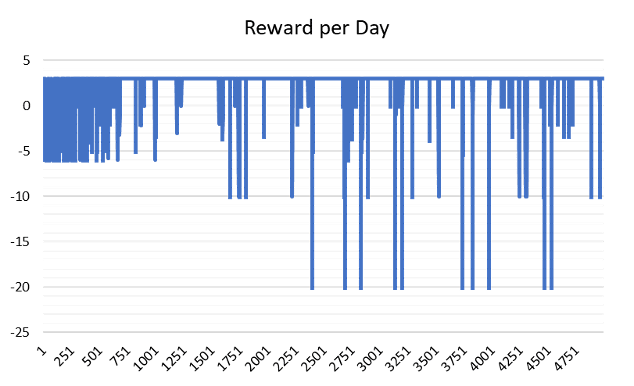
\includegraphics{004_team_2_agent_design/rewardperday}
\caption{Reward per day.}
\label{rewday-team2}
\end{figure}

\begin{figure}
\centering
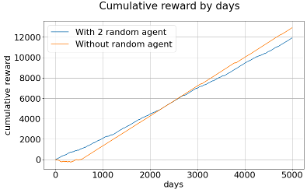
\includegraphics{004_team_2_agent_design/cumrewardbydays}
\caption{Cumulative reward against days.}
\label{cumday-team2}
\end{figure}

Figure \ref{rewday-team2} is the result of a simulation for 5000 days without random agents. Reincarnation is allowed in this simulation. 

It can be observed that during approximately the first 500 days, the agent consecutively gets punished and the reward fluctuates frequently. Then, it starts to find the way to cater to the design of reward function, and despite the instability caused by randomness in the tower, the reward function tends to be smoother, as the changes in reward function occur less frequently. 

In addition, in Figure \ref{cumday-team2}, we can find that the cumulative reward increases at a nearly steady speed after fluctuation. The turning point is approximately 500 days as well.

Thus, it can be concluded that under the configuration of this experiment, the policy of the agent is able to converge at around 500 simulation days. This means that the agent manages to find the best policy to maximise the reward he can get and persist this policy to consecutively achieve better rewards. Within its context and ability, it has achieved the Pareto optimal level for individual utility.

The verification of convergence is fundamental to the presentation of our results. All the results introduced next are based on our successful implementation of the learning algorithm.

\subsection{Random Agent}
The effect of having random agents in the tower to our agent is discussed in the following. The random agent takes food randomly with the range between 1 till max food available on the platform. This strategy can result in the random agent overeating, which will reduce collective utility. This is due to total food allocation equal to $(\textrm{FoodPerAgentRatio}) * (\textrm{number of agent})$ while the random agent will intend to eat between 1 and total food allocation.
\begin{figure}
\centering
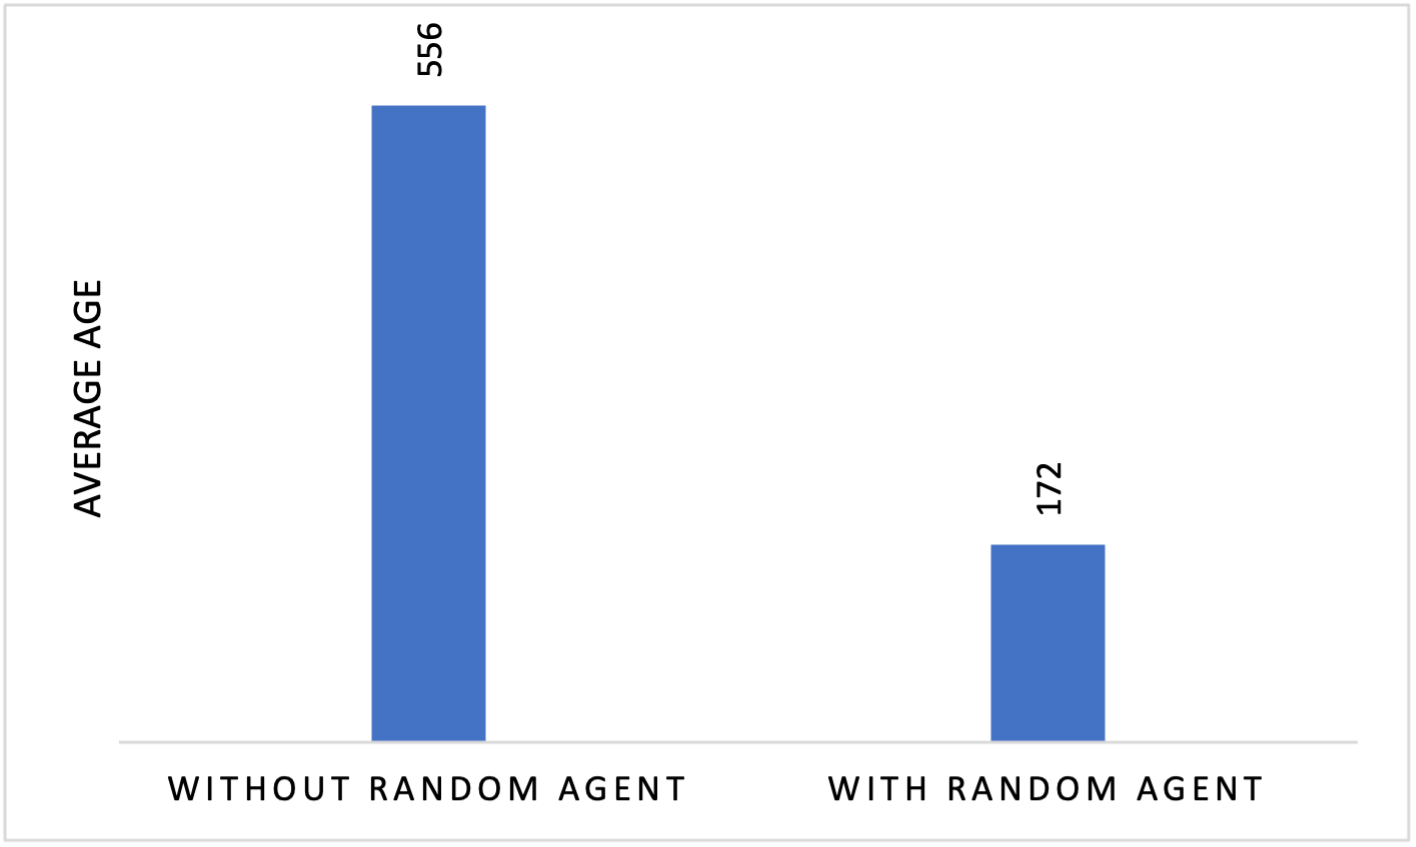
\includegraphics{004_team_2_agent_design/team2avage}
\caption{The average age of Team 2 Agent.}
\label{team2av}
\end{figure}
\begin{figure}
\centering
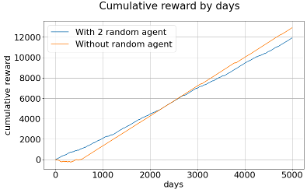
\includegraphics{004_team_2_agent_design/cumrewardbydays}
\caption{Cumulative reward by days.}
\label{cumreward-team2}
\end{figure}
\begin{figure}
\centering
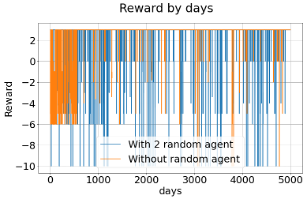
\includegraphics{004_team_2_agent_design/rewardbydays}
\caption{Reward by days.}
\label{dayreward-team2}
\end{figure}
\begin{figure}
\centering
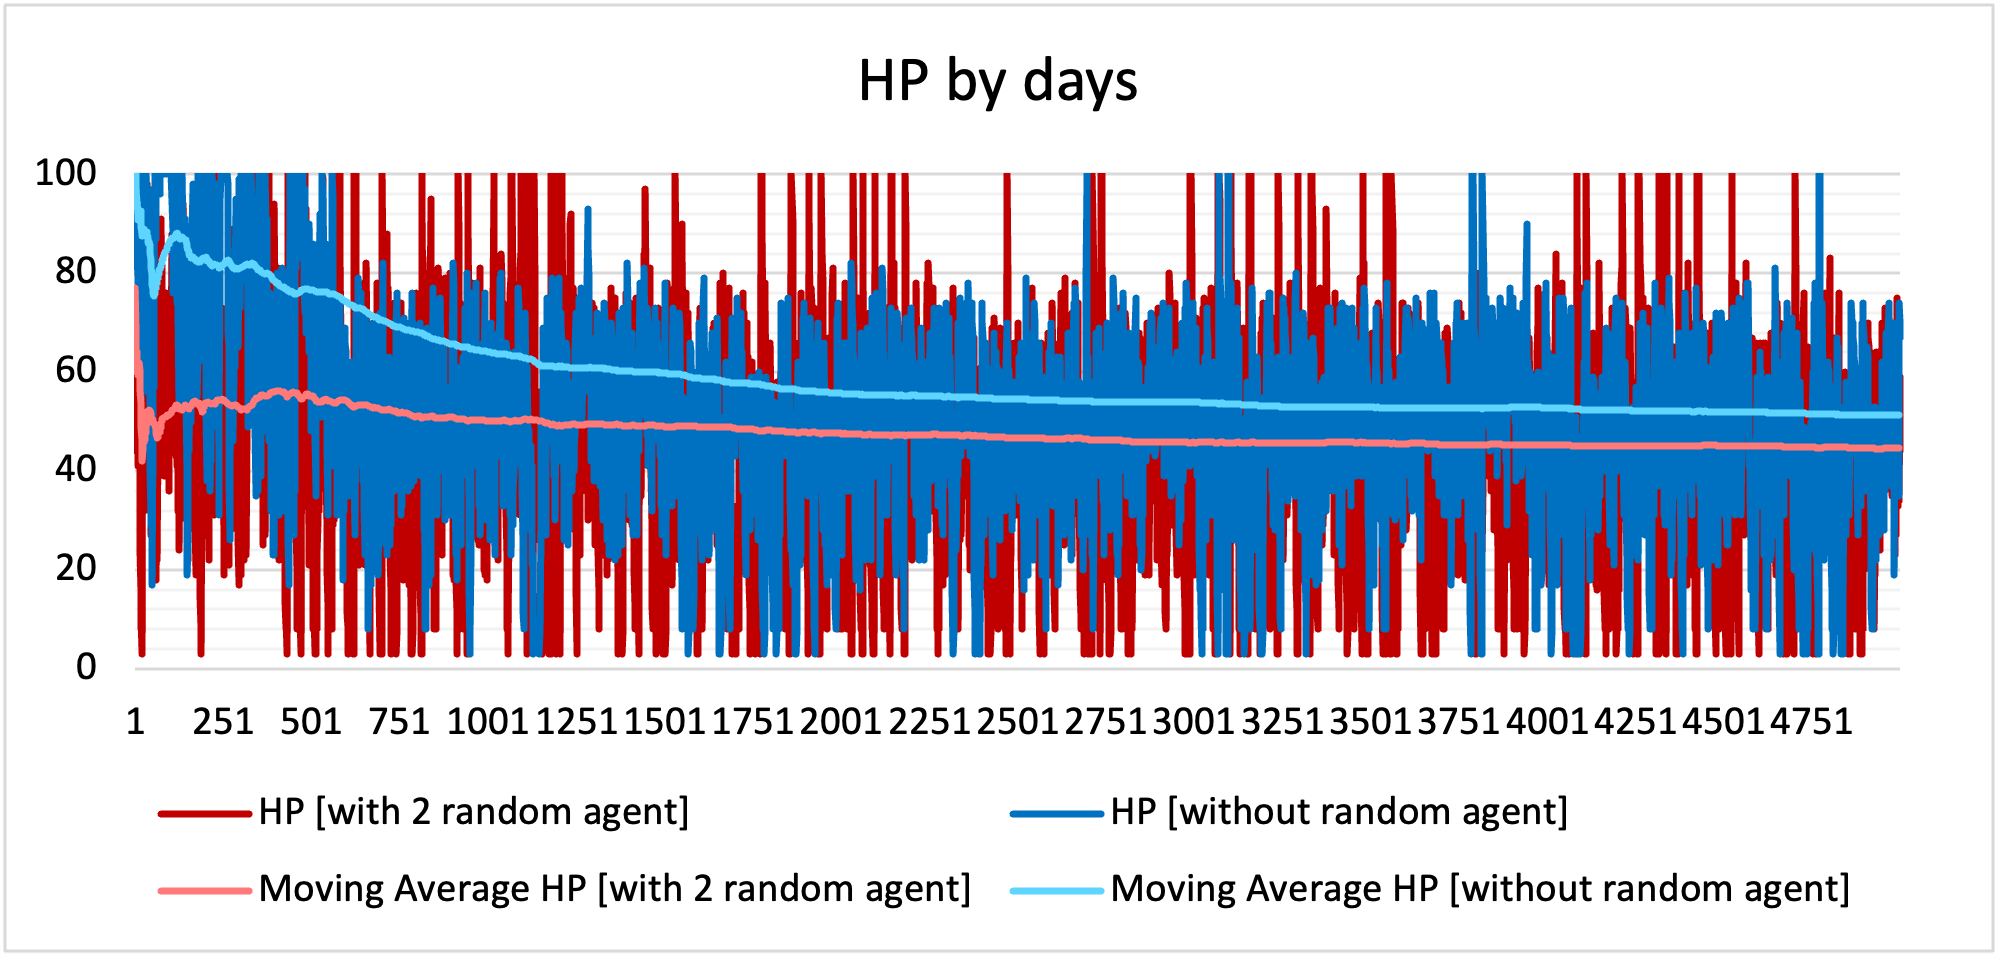
\includegraphics{004_team_2_agent_design/hpchange}
\caption{The change of agent HP by days.}
\label{hpchange-team2}
\end{figure}

With the inclusion of the random agent(s) in the tower, the average age of our agent is observably decreased from 556 days to 172 days in Figure \ref{team2av}. This demonstrates the direct implication of collective utility on an individual agent; regardless of individual strategies, a rogue agent which does not keep the macro-level goal of collective utility will hamper the individual utilities of the other agents. 

The results in Figure \ref{cumreward-team2} and Figure \ref{dayreward-team2} are from a reincarnation-allowed simulation with only one agent of our team. In Figure \ref{cumreward-team2}, our agent with 2 random agents performs better than without random agent before 2500 days. However, when comparing with the plot of reward by days (Figure \ref{dayreward-team2}), our agent with 2 random agents has a greater total reward penalty. This is due to the randomness introduced by the random agent, causing the learning process of our agent is insufficient. On the other hand, without implementing the random agent in the tower, our agent able to learn after being deployed.

When there are random agents in the tower, our agent tends to overeat more frequent to confront the effect from the random agent in Table \ref{hpchange-team2}. However, the moving average HP of our agent is lower compared to without random agent.

To conclude, the random strategy of the random agent detriments the learning process of our reinforcement learning agent. The main goal for our agent is to change its strategy according to the environment to survive, the randomness effect from random agent cause confusion for our agent as the reward may be different for the same action our agent has taken at the same state. This leads to a poor learning environment for our agent and removing random agent during the learning process of our reinforcement agent is suggested.

\subsection{Average HP}
\begin{figure}
\centering
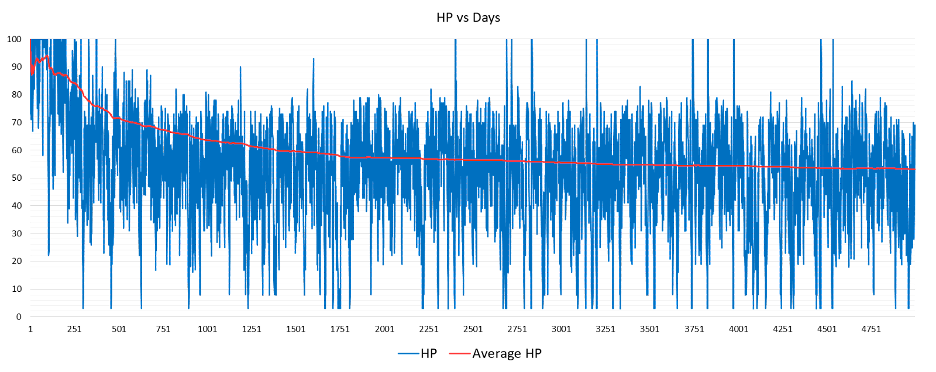
\includegraphics{004_team_2_agent_design/avhpdays}
\caption{Average HP against days.}
\label{avhp-team2}
\end{figure}

The results in Figure \ref{avhp-team2} are from an experiment without random agents. Only one agent of our team is included, and reincarnation is allowed. 

Following the design in the reward function, the HP of our agent is learnt to retain under 80. It does not choose to stay as close as possible to the upper HP limit 80. Instead, the agent decides to maintain the HP around 55 on average. 

This may indicate that staying at a high HP level may not be a good surviving strategy in the tower. 

\subsection{Reincarnation of Agent}
The results of this part are from experiments without random agents and only one agent for our team is involved.

With reincarnation, the agent will not be able to lose its memory or experience after each death, which is a basic factor for a learning algorithm. In our hill-climbing Q-learning, the reincarnation allows for the retention of the Q table and policy table when the agent dies. 

From the comparison of Figure \ref{rewday-team2} and Figure \ref{cumday-team2}, it seems that there is no difference between the agent with and without reincarnation in terms of the total death and surviving days. The agent without reincarnation can live as long as the agent with reincarnation although it cannot inherit. This is partly because that, due to our effort in design to minimize the model complexity and maximize the convergence speed, our agent learns fast and normally it will converge within 200 days. Thus, if the agent can avoid death in the first 200 days, which is of high probability, it can live for a long time with the learnt strategy. Its policy will be self-optimized consistently as long as he is alive. 

This can be further explained by examining the Figure \ref{team2av} graph that specifically shows the 13th life of the non-reincarnating Team 2 agent from Figure \ref{rewday-team2} Here the agent although not reincarnated from a previous life still shows a cumulative reward curve that eventually shows a linear increase, meaning it has found a near optimal policy through dynamically adapting fast enough.

In addition, the loss of reincarnation still casts some instability. From Figure \ref{cumreward-team2}, we witness that the HP of the agent fluctuates more heavily if it cannot reincarnate. This may result from the fact that the most unstable duration for the Q-learning algorithm is the learning period. If the agent cannot reincarnate, it has to experience the learning period again every time it dies which will definitely introduce more unstable factors. 

\begin{figure}
\centering
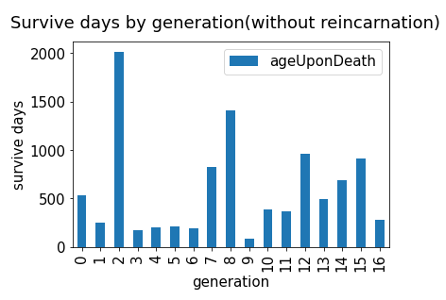
\includegraphics{004_team_2_agent_design/suvdayworein}
\caption{Surviving days of each live without reincarnation.}
\end{figure}

\begin{figure}
\centering
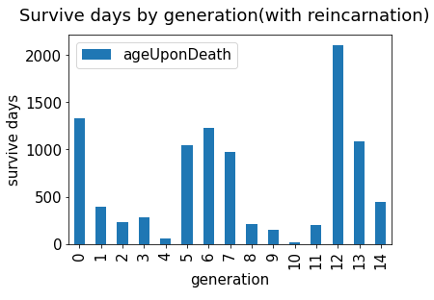
\includegraphics{004_team_2_agent_design/suvdaywrein}
\caption{Surviving days of each live with reincarnation.}
\end{figure}

\begin{figure}
\centering
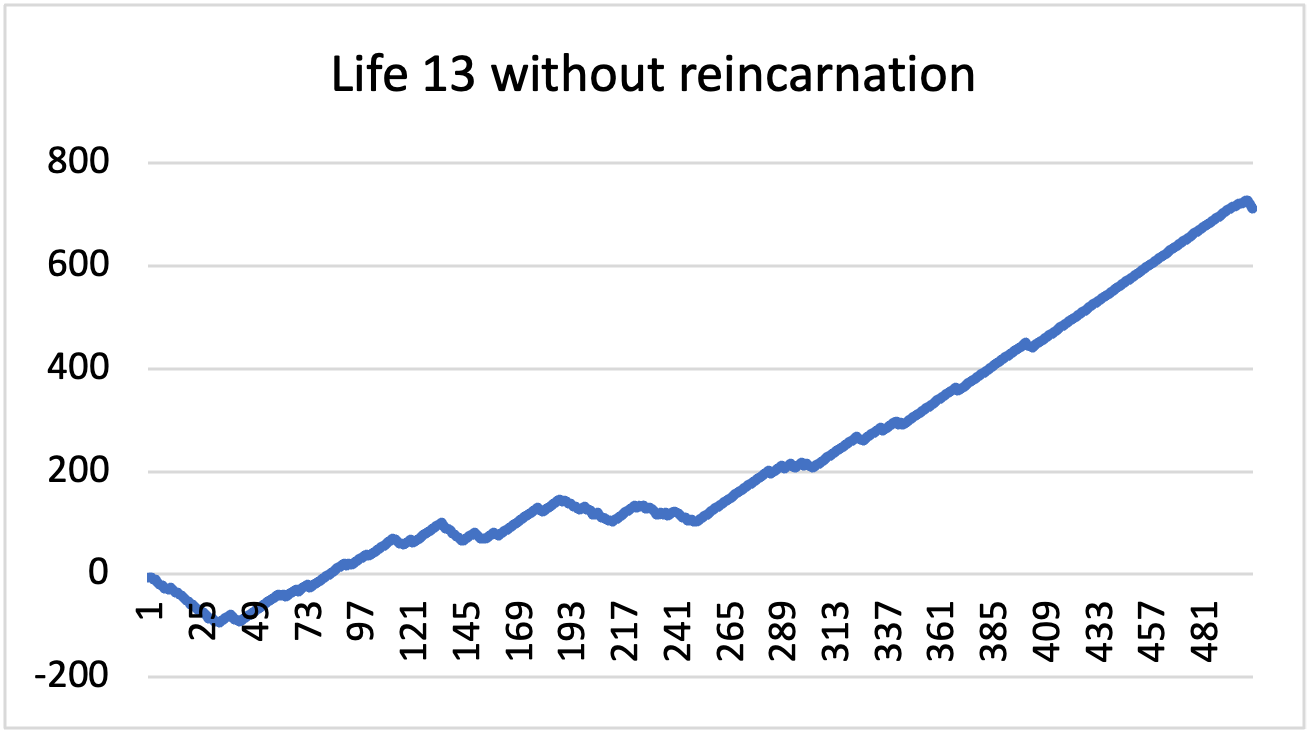
\includegraphics{004_team_2_agent_design/cum13team2}
\caption{Cumulative reward of 13th Team 2 agent life without reincarnation from the previous figure.}
\end{figure}

\begin{figure}
\centering
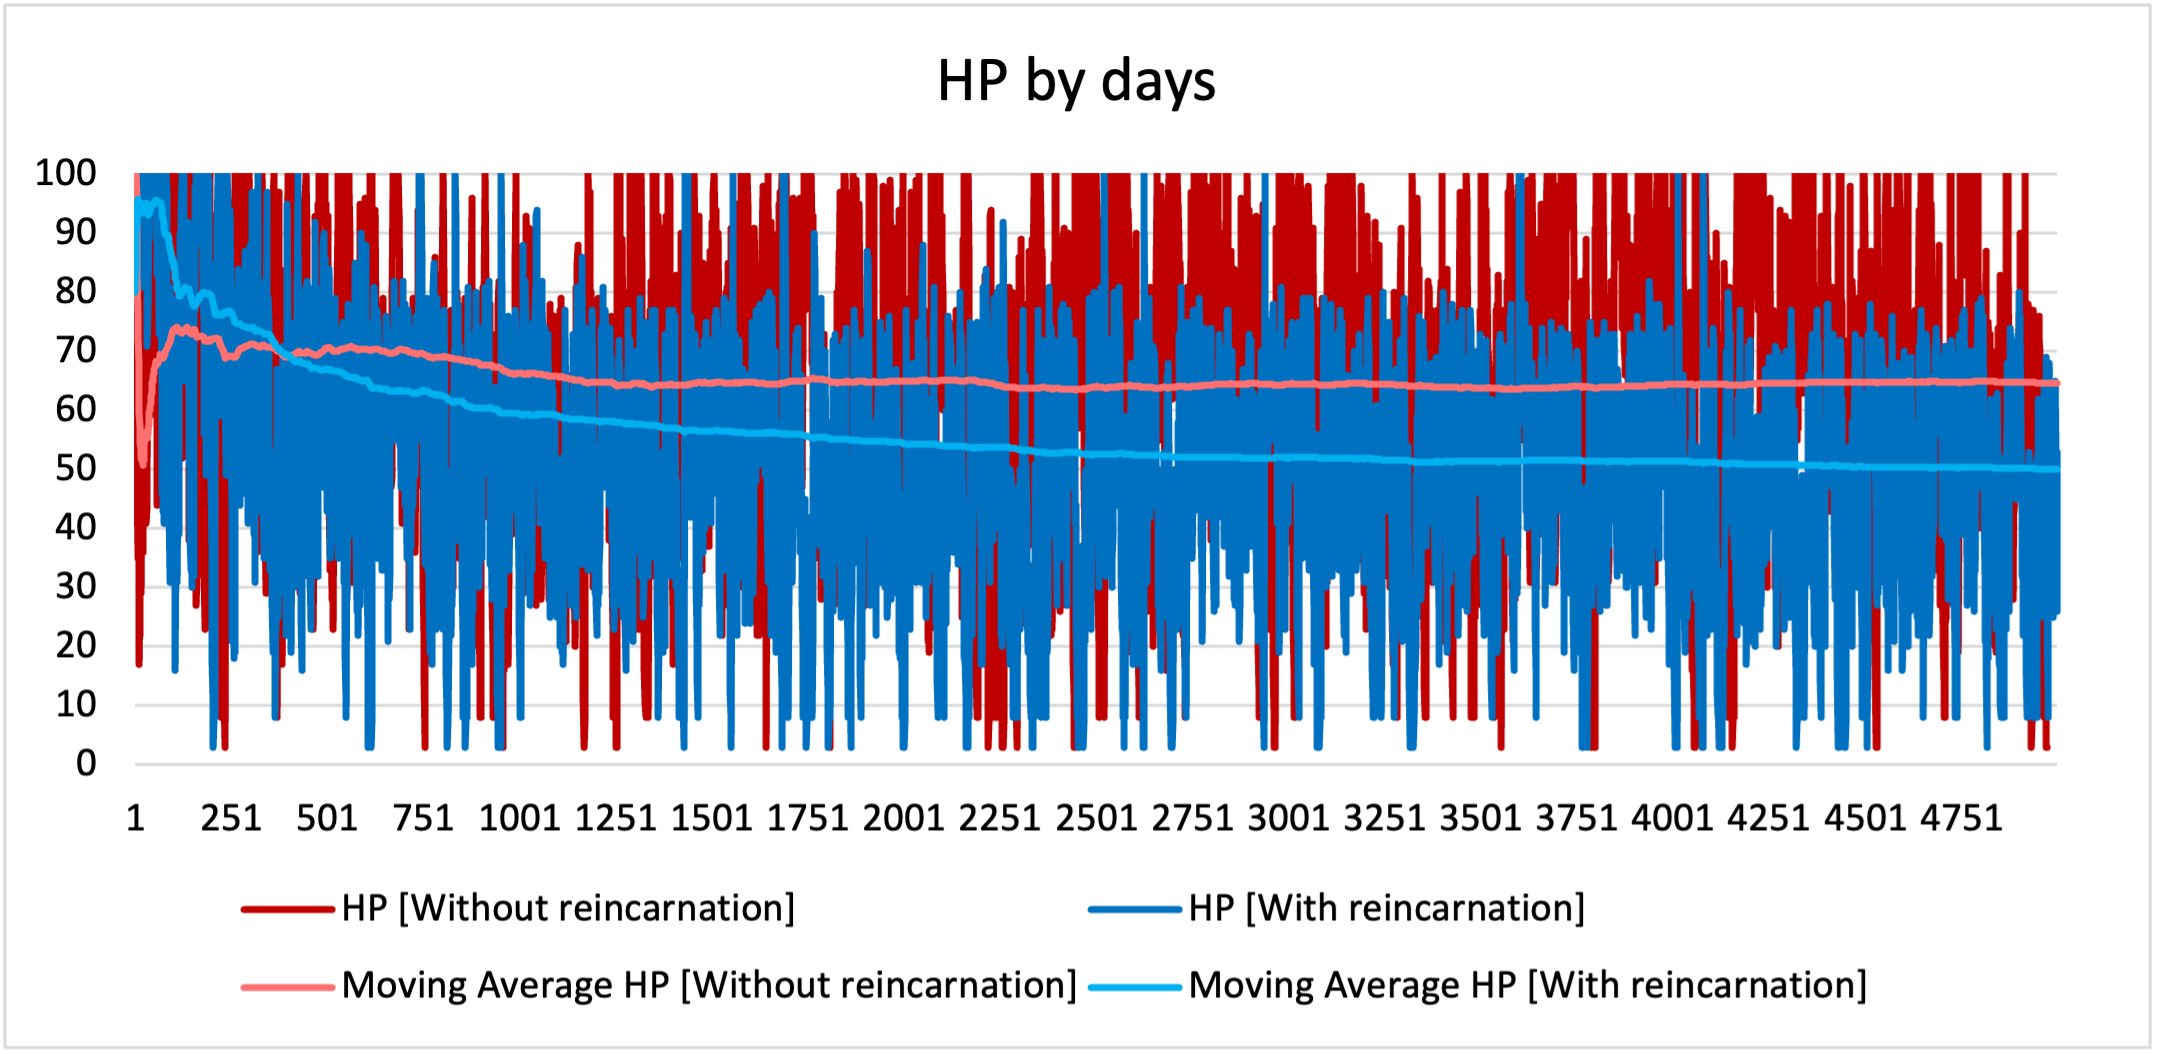
\includegraphics{004_team_2_agent_design/hpdaysteam2}
\caption{The change of HP by days with and without reincarnation.}
\label{hpdaysteam2}
\end{figure}

Enabling reincarnation can let the agent pass its learnt knowledge to its child, while disabling the reincarnation will lead to a tumultuous relearning process for every generation. Enabling the reincarnation of our agent is important as it let our agent learn from the reward and inherit the experience from its predecessor. 

As a conclusion to reincarnation, the most important impact of reincarnating the Team 2 agent is not an increase in its own performance as it learning rate is fast enough for the average life duration. The real trade off with reincarnation is the effect it has on the tower’s other agents. The average HP is lower with reincarnation as can be seen in Figure \ref{hpdaysteam2}, and so the other agents benefit from this much more. As previously discussed, maintaining the Pareto optimal individual utility will allow for an increase in each other agent’s individual utilities, and thus the collective utility.

\subsection{Self-Organising Ability}
A tower that can self-organise has reached an equilibrium where agents no longer die and instead are able to survive all together based on their adaption to each other and the environment. As discussed in Section \ref{team2-organisation} this generally would occur when all the agent behaviours have assimilated and converged to become one and the same. Thus, it is in our interests to test a scenario with a tower full of the same agent type. To test Team 2 agents’ own self-organising ability, towers with different number of Team 2 agents present where tested.

The results in Figure \ref{251team2} shows that the Team 2 agent does indeed have a huge impact on the towers performance. The more Team 2 agents present in the tower the fewer deaths the tower would have. But with this reading alone its not possible to determine if the Team 2 agents actually has a self-organising ability as there is no way of knowing when the last agent died in each run. Figure \ref{252team2} on the other hand shows how a tower consisting only of Team 2 agents eventually reached an equilibrium point where all agents stayed alive. As such the design of the Team 2 agent showed self-organising ability with its Q-learning PHC reinforcement learning strategy.

\begin{figure}
\centering
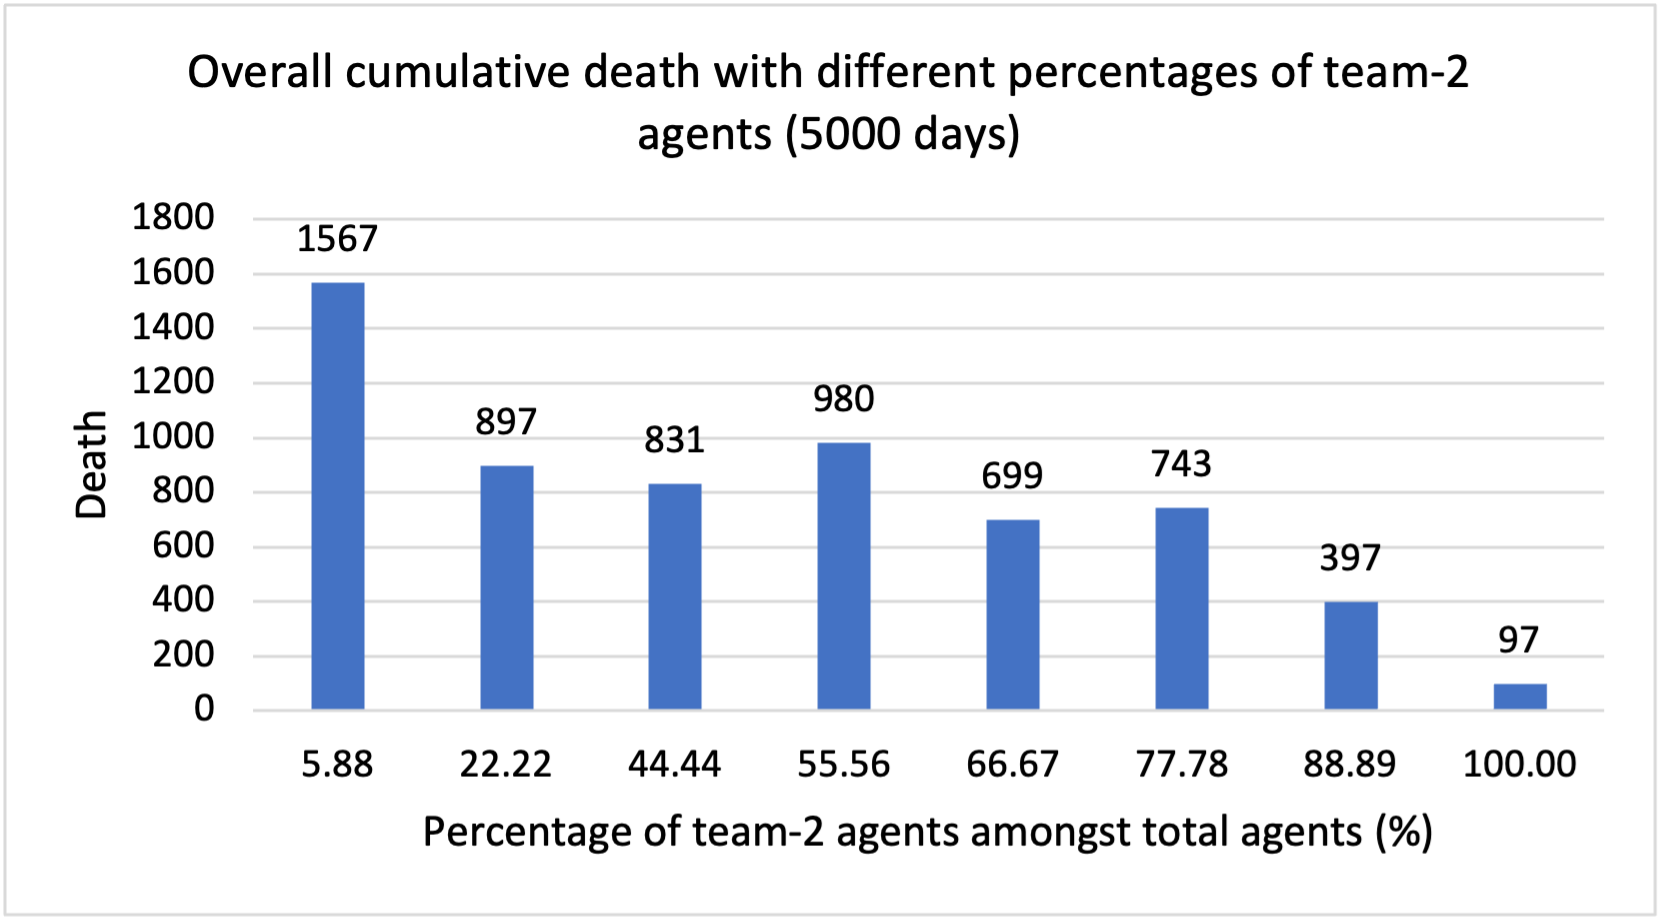
\includegraphics{004_team_2_agent_design/251team2}
\caption{1 Shows the cumulative deaths of a towers with varying percentage of total agents being Team 2 agents. Total agent count is 18 agents.}
\label{251team2}
\end{figure}

\begin{figure}
\centering
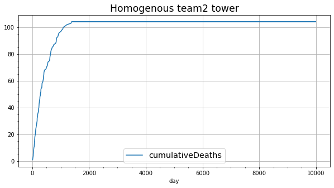
\includegraphics{004_team_2_agent_design/252team2}
\caption{tower of only Team 2 agents reaches a point where all agents stays alive.}
\label{252team2}
\end{figure}

\subsection{Learnt Policies}
\begin{table}
\centering
\caption{Policy of agent when HP is 0-10.}
\label{lowhp-team2}
\begin{tabular}{@{}ll@{}}
\toprule
HP   & Average Food decided to take \\ \midrule
0-10 & 27.3                         \\ \bottomrule
\end{tabular}
\end{table}
Table \ref{lowhp-team2} shows that when the HP of agent is low, the agent tends to take in as much food as he can to survive, as it must prioritise its individual survival and cannot consider other lofty altruistic goals.

\begin{table}[]
\centering
\caption{Policy of agent when HP is 10-20.}
\label{midhp-team2}
\begin{tabular}{@{}lll@{}}
\toprule
HP    & Food on the platform & Food decided to take \\ \midrule
10-20 & 0-20                 & 13.2                 \\
10-20 & 20-30                & 7.1                  \\
10-20 & 30-100               & 23.9                 \\ \bottomrule
\end{tabular}
\end{table}

From Table \ref{midhp-team2}, it is prominent that the agent is still in a dangerous HP range. When there is not much food on the platform, the agent decides to eat more to survive.
When the food on the platform is 20-30 which is still not safely sufficient, even though its HP is not high enough, the agent seems want to leave food for others. The agent probably considers that in such case, leaving food for others can be a better choice because if some agents fall into the critical level, they may need more food to reach the weak level than what they need now. Perhaps it has developed some form of empathy, where it perceives that other agents may be in similar if not more dire situations. 

When the food is abundant on the platform at this HP level, the agent takes in more food. This might be a strategy to prevent being allocated to lower floors on the next day since its HP is still near critical level.

\begin{table}[]
\centering
\caption{Policy of agent when HP is 20-30.}
\label{2030-team2}
\begin{tabular}{@{}lll@{}}
\toprule
HP    & Food on the platform & Food decided to take \\ \midrule
20-30 & 0-20                 & 16.1                 \\
20-30 & 20-40                & 6.1                  \\
20-30 & 30-50                & 21.0                 \\
20-30 & 50-100               & 5.0                  \\ \bottomrule
\end{tabular}
\end{table}

Table \ref{2030-team2} shows the decisions of the agent when HP is in 20-30 level. It is observed that its policy at this level is quite similar to that at HP 10-20. It still chooses to ensure the survival of itself when the food is not enough. When the food is above the level of scarce, it still decides to eat less and leave the food for others. In addition, when there is 30-50 food on the platform, it decides to eat more again, but when the food on the platform is more than this it chooses to barely eat. It seems that from the experience of agent in HP 20-30, 30-50 food on the platform can be a dangerous indication that it may starve or lose HP in the next few days, so he tends to supply himself for the future. And the agent considers it unnecessary to eat much when there is abundant food on the platform, due to the reward function penalties.

\begin{table}[]
\centering
\caption{Policy of agent when HP is 30-100.}
\label{30100-team2}
\begin{tabular}{@{}ll@{}}
\toprule
HP     & Food decided to take \\ \midrule
30-100 & 5.0                  \\ \bottomrule
\end{tabular}
\end{table}

Table \ref{30100-team2} shows that when the HP of agent is larger than 30, it tends to eat the minimum amount of food and leave the food to others.

In summary, from the observations gathered, the learnt policy of the agent follows certain patterns:
\begin{itemize}
	\item The priority is the survival of itself; the tower scenario is often too unpredictable to switch to more altruistic objectives
	\item Leaving food for others when the food is not sufficient tends to bring more collective benefit in the long term
	\item Maintaining HP over 30 is safer for the survival of agent and is more likely to result in a Pareto optimal value for individual utility
\end{itemize}



\chapter{Team 3 Agent Design}\label{team_3_agent_design}

\section{The Agent}\label{the_agent}
%%Some general description of the agent

\subsection{Agent knowledge}
Agent 3 will be able to remember facts in order to make decisions. The variables in their memory are:
\begin{enumerate}
    \item \texttt{floors []int}: stores the floors the agent has been in before. This information is used on reshuffles to set our mood. 
    \item \texttt{lastHp int}: stores the last recorded HP value. Currently used to check a new day has started.
    \item \texttt{friends []string}: stores the ID of the agents they have met before. The agent is aware of the people they have met during their time in the tower. Their Id is stored in this slice. 
    \item \texttt{friendship []float}: stores our affection for the agents we have met. Affection range is 0-1 (0 = dislike, 1 = like). The position at which an agent's id is stored in our \texttt{friends[]} slice corresponds to the position in which the affection we have for that agent is stored in the \texttt{friendship[]} slice.
    \item \texttt{floorBellow string}: stores which agent is living on the floor below us until the next reshuffle.
    \item \texttt{floorAbove string}: stores which agent is living on the floor above us until the next reshuffle. 
  \end{enumerate}

subsection{Agent decisions}
Agent 3 will be able to take decisions when receiving messages or after signing treaties and store these until they eat. This information is used to symbolize a predetermined decision has been taken instead of “impulsively” eating food depending solely on our hunger and state of mind.
\begin{enumerate}
    \item \texttt{foodToEat int}: stores how much food we have decided to eat in the next eating period.
    \item \textt{foodToLeave int}: how much food we have decided to leave. It is necessary in case we want to: E.g eat 6 food and leave at least 10 food but when the platform arrives we see that it has 13 food. Both statements cannot be fulfilled and so we must prioritise one.
\end{enumerate}

subsection{Agent variables}
Agent Variables
Agent 3 will act differently depending on three different variables that define them, which will give the agent different personalities.
\begin{enumerate}
    \item \texttt{stubbornness int}: defines the likelihood of the agent to read a message. E.g: Stubbornness = 20 means there is a 20\% chance that the agent will ignore the message.
    \item \texttt{morality int}: defines  the willingness of the agent to help others, in other words, how much you care about other agents in the tower. 
    \item \texttt{mood int}: defines how likely the agent is to do things, it will affect its decision-making process.
\end{enumerate}
For the purpose of this agent, we will define personality as the individual differences in characteristic patterns of thinking, feeling, and behaving, as defined by the American Psychology Association. The traits that define an agent's personality are mutable, making our agent adapt its personality depending on the circumstances. 

\chapter{Team 4 Agent Design}\label{team_4_agent_design}

\section{Strategy Overview}
The overall agent strategy was determined by an evolutionary algorithm (see overview in \Cref{fig:evolutionOverview}) which allowed the agent to preemptively adapt to unknown environments. The evolutionary algorithm was further complemented by a trust score, which acted as a measure of the agent's perception of the trustworthiness of other agents in the tower. Additionally, the agent was given a cravings parameter which simulated how hunger would affect a human in the real world. This created a well-rounded agent that was able to dynamically adapt to the changing environment in order to survive. 

\begin{figure}[htb]
    \centering
    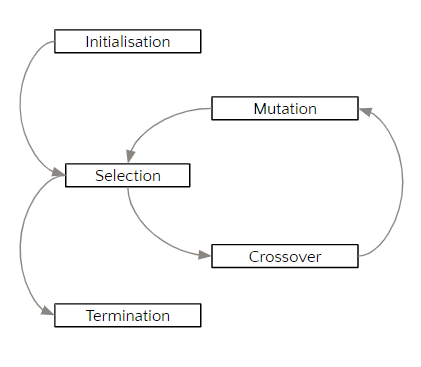
\includegraphics{006_team_4_agent_design/assets/evolution_overview.png}
    \caption{Overview of evolutionary algorithm.}
    \label{fig:evolutionOverview}
\end{figure}

\section{Evolutionary Algorithm}

In the fundamentals of evolutionary algorithms, every agent has a set of genes (or genotypes), which can express themselves (as phenotypes) in the way the agent interacts with its surroundings. Therefore, the aim is to find the optimal genotypes that will give phenotypes that are deemed to be favourable. This is implemented by seeing the performance of an agent according to a particular metric. This way the effect of each phenotype (and therefore underlying genotype) is put into perspective and ranked against the others. The most successful agents survive, while the less performant ones are killed off. When the surviving population reproduces, the resulting offspring will share the genes of both their parents, meaning they will have a mix of the most successful genotypes. Furthermore, there are some offspring with mutated genes and some that have identical genes to the previous generation for genetic variation. With this new population, the process is repeated to iteratively create more successful populations, as illustrated in \Cref{fig:team4evolve}.

\begin{figure}[htb]
    \centering
    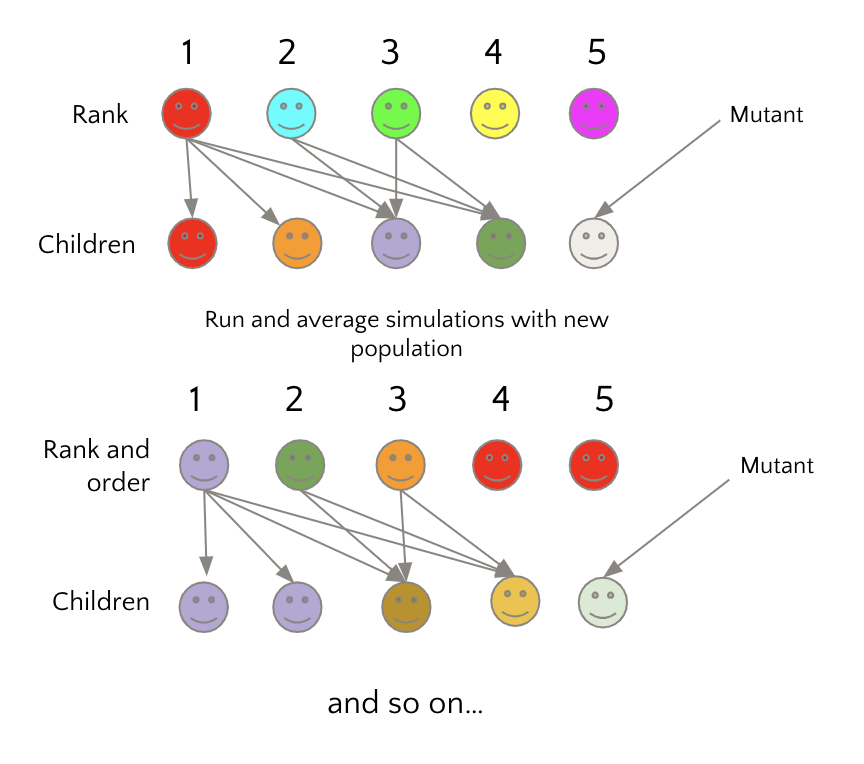
\includegraphics[width=0.7\textwidth]{006_team_4_agent_design/assets/evolve.png}
    \caption{Population selection process in an evolutionary algorithm.}
    \label{fig:team4evolve}
\end{figure}

Hence, with the use of an evolutionary algorithm, the final agent was the culmination of multiple generations of populations, with the genes of successful ancestors having been propagated and mixed. This meant it was a well-adapted agent which was robust to the many environments it could encounter in the tower. 

\subsection{Agent Genotypes}
To use evolutionary algorithms optimally, the genotypes that evolve should be well defined. This section outlines the two genotypes that were chosen as they were deemed to have the most effect on the survival of an agent in the system.

\subsubsection{FoodtoEat}\label{FoodtoEat}
\texttt{FoodToEat} was the amount of food the agent would eat on any given day of the simulation. Given the HP update curves in \Cref{updateHP}, it can be noted that any consumption past the threshold of 60 food had little to no effect on the HP gain of the agent. This meant that eating any more than that amount was wasteful and sub-optimal, so during the training process the algorithm was capped. This meant that the process could never learn to eat a value above 60, just as it could not learn to eat a value below 0.

\subsubsection{WaitProbability} \label{waitProbability}
\texttt{WaitProbability} was the probability that the agent would not eat on any given day of the simulation. This is a probabilistic way of creating the agent, which is ideal to replicate the unpredictability of the real world. Having other implementations such as a hard-coded number of days to wait would give a much more robotic and predictable agent. This was especially apparent when initialising homogeneous populations of the evolutionary agent in the tower since they would all wait and eat at exactly the same times. With the probabilistic approach, this is not the case, and there was still a way for the agent to express a wanting to abstain from eating food on a particular day.

\subsection{Health Levels}
In order for these genotypes to be viable in the learning process, the values they could take had to be limited. The \texttt{FoodToEat} and \texttt{WaitProbability} were inherently limited to lie between 0-60 and 0-100 respectively, but there were many conditions under which the agent would have to choose between these values. It was decided that the agent's HP was the most apt factor in its decision making process. Hence, the agent's HP was divided up into different bands as a means of classifying the agent's current health into broader categories. The division resulted in four levels being created: Critical, Weak, Healthy and Strong with the range of HP corresponding to each level displayed in \Cref{tab:healthLevels}.

\begin{table}[htb]
    \centering
    \begin{tabular}{| c | c |}
    \hline
    Health Level & HP Range \\
    \hline
    \hline
     Critical & 3-9 \\ 
    \hline
     Weak &  10-39\\  
     \hline
     Healthy &  40-69\\
     \hline
     Strong & 70-100 \\
     \hline
    \end{tabular}
    \caption{Overview of the different health levels and their corresponding HP ranges.}
    \label{tab:healthLevels}
\end{table}

In each health band, the agent would consume a certain amount of food with a given probability of waiting before eating. The division of HP into broader bands reduced the complexity of the learning process greatly as compared to when optimising food intake for every possible HP value, and was therefore chosen as a good compromise.

\subsection{Cravings}

To implement a more realistic and life-like element to the agent, a cravings trait was added. The cravings of the agent would be increased as the desire for food increases and decreased otherwise.

Cravings directly effected the \texttt{waitProbabilities} put forward in \Cref{waitProbability}. As days pass without seeing food on the platform, the agent's craving increases, and in turn, its probability of waiting to eat decreases. The intuition behind this was that as more days pass without seeing food, the agent should eat when it can as there may not be many opportunities to do so in the future and may potentially lead to death.\newline

An agent's craving was altered in a few different scenarios:
\begin{enumerate}
    \item Food not seen on the platform - If the agent has not seen food in $x$ days, cravings is increased by $x$. Otherwise, the craving is decreased by two for everyday food is seen on the platform. 
    \item Eating food - When the agent eats food, craving is decreased proportionally to the amount of food the agent has eaten \emph{i.e.} $cravings = cravings \left(1 - \frac{foodeaten}{desiredfood}\right)$
\end{enumerate}

This enabled the agent to perform house-keeping as it reduced the likelihood of a scenario where the agent does not eat for long periods of time, preventing self-inflicted damage as a result of \texttt{waitProbability}. 

It should be noted that the training process did not learn the values to assume in the critical region. These values were instead hard-coded as the agents `survival instinct', whereby it ate what it needed to leave critical health. This added a component of self-healing to the agent.

\subsection{Agent Performance Metrics}
\begin{table}[hbt]
    \small  
    \centering
    \resizebox{\textwidth}{!}{%
    \begin{tabular}{| m{5em} | m{13em} | m{14em} |}
    \hline
    Averaging method & Advantages & Disadvantages  \\
    \hline
    \hline
        Global Lifespan & 
        - Attempted to maximise lifespan of all agents including itself 
        
        - Struck a balance between self preservation and global welfare. 
        & 
        - Didn't reach optimum strategy with no deaths
        
        - Agent had little effect on global lifespan. \\
        \hline
        Team Four Agent Lifespan & 
        - Maximised agent 4 survival (attempted to satisfy itself)
        
        - Actions of others had less effect on survival of agent. 
        & 
        -  Disregarded other agents in the tower
        
        - Failed to create stable system as all food was consumed by agent. \\
        \hline
        Other Agent Lifespan & 
        - Attempted to reach optimum state of co-operation
             
        - Worked for the betterment of society (for the satisficing of each agent).
        &
        - Put itself at risk while eating minimal amount of food
             
        - Agent had little effect on global lifespan. \\
        \hline
    \end{tabular}}
    \caption{Pros and cons of different averaging methods chosen for agent parameter optimisation.}
    \label{tab:lifespanAveraging}
\end{table}

When training the agent, there were multiple ways to interpret any given metric. For this project, it was decided that the metric that gave the most accurate depiction of agent fitness was their lifespans. For this reason, average lifespans were used during the training process, but even so, there were many options for how to take these averages. The pros and cons of our chosen averaging methods are given in \Cref{tab:lifespanAveraging}.

The agent was trained to determine three personalities: selfish, neutral and selfless. The selfish nature of the agent was designed for self-prioritisation over community welfare. The selfless configuration was trained to optimise the global life expectancy whereby the agent would try to reduce global deaths per iteration. The neutral configuration aimed to strike a balance between the two previous configurations, trying to optimise overall life expectancy, inclusive of itself. Through this method, the agent has the capabilities to maximise its utility at the micro level and sustainability at the macro level.

\section{Message Passing}
To create an agent that can self-organise according to its neighbours, communication was vital so that its actions would vary according to a changing environment. Both message passing, and treaties had been implemented to account for the many possible situations that could affect the agent. 

\subsection{Simple Messages} \label{team4SimpleMessages}
For simple communication, the agent was able to both send messages and handle the messages received from other agents.

\subsubsection{Handling Message Generation}
There were two scenarios the agent considered when determining what message it would want to send. The first was when the agent’s health status had reached critical. A message was sent to the floor above requesting them to leave just enough food for the agent to survive. Messages were also sent so that the agent could learn about the amount of food another agent (on a different floor) intended to take, as well as the amount of HP they had. Not all recipients would respond to these requests, so to maximise the agent’s interaction and learning, it yelled across multiple floors, both above and below.

\subsubsection{Handling Received Messages}
Many other agents from multiple floors were likely to send their own requests, so various handler functions were implemented to determine the preferred response. When a message was first received, it was stored into one of two memory buffers. One for recording messages requesting a particular amount of food to be left, and another for other message types. Since the agent could only respond to one message per tick in the simulation, it prioritised those asking for food to be left first. To determine if the agent should accept the request, it waited for the platform to reach its own floor. It then compared if the available amount on the platform after the agent ate was greater or equal to the amount being requested. If this was true, it left that amount and sent a response saying yes. For all other message types, the agent replied honestly to a given query. 

\subsection{Treaties} \label{team4Treaties}
The agent accepted any subset of treaties that were in line with its own goals. The first few conditions were all dependent on the availableFood. In the case that the agent was within a threshold of the critical region (this being the critical health level multiplied by 2), the corresponding treaty was rejected. The agent also rejected any treaties where the condition was dependent on having available food less than a certain amount. Finally, all treaties requiring the agent to leave food less than the critical amount were rejected, so as to afford agents on lower levels of the tower the opportunity to survive if they were in critical condition. 

Similarly, treaties were also subject to the condition of HP. The agent rejected all treaties where the conditional HP was less than the critical band. Here, the agent would be at the point of desperation and should not be forced into any action. Additionally, treaties may have been requested where the condition of the agent was required to be less than a certain HP, or the agent was required to be placed on a higher floor number. These would lead to a significant disadvantage for the agent as treaties are binding. Consequently, treaties with these conditions were all rejected. When the duration was greater than the maximum number of days in critical, it could lock the agent into a forced action resulting in its death. To ensure this didn't happen, the agent rejected all such opportunities. 

The agent also propagated accepted treaties, giving other agents the option to follow a similar ideology to its own. The agent could then enforce it's influence on the social order within the chaos of the tower. On the other hand, treaties that were not accepted were not further propagated. This was because the agent did not want to spread methods that were in detriment to it's own as this would pose a risk to the social order enforced by the agent itself.

\section{Trust Score}
The trust score was a parameter that allowed a more dynamic approach to be built on top of the relatively static evolutionary algorithm. The agent used this trust score to build a global trust network based on its local interactions using the message passing and treaty-based techniques mentioned in \Cref{team4SimpleMessages} and \Cref{team4Treaties}. The trust score allowed the agent to alternate between the three personalities: selfless, neutral and selfish. \Cref{fig:team4updateHP} shows examples of certain trust score updates where the agent was able to vary its own configurations after altering its trust score parameter. This gave the agent an element of self-optimisation as it was allowed to adapt to information gained from its environment and other local interactions. 

\begin{figure}[htb]%
    \centering
    \subfloat[\centering Decrease in trust]{{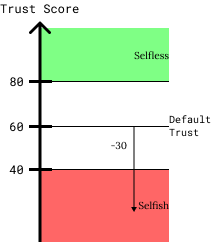
\includegraphics[width=0.3\linewidth]{006_team_4_agent_design/assets/selfish.png}}}%
    \qquad
    \subfloat[\centering Increase in trust]{{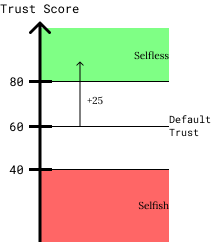
\includegraphics[width=0.3\linewidth]{006_team_4_agent_design/assets/selfless.png}}}%
    \caption{Change in agent configuration as a result of global trust score.}%
    \label{fig:team4updateHP}%
\end{figure}

Trust score for an agent was increased through a multitude of interactions. As the system was designed to be honest, the agent increased trust score when the floor above took a certain amount of food that was deemed to be an acceptable value (less than the maximum food taken in the selfish configuration) and communicated this to the agent. Additionally, when the floor below left a certain amount of food, the agent also increased its trust score.

In the cases where the floor above left a certain amount of food and the agent below also took a certain amount of food, the agent did not instantaneously increase the trust score. Instead, the agent verified that the agents above and below followed through with the actions mentioned through the \texttt{verifyResponses} function. The agent used the function once it received replies to \texttt{RequestLeaveFood} and \texttt{RequestTakeFood} messages. Whenever a message was sent, it was stored by the agent. This allowed the agent to correspond replies and responses to the appropriate sent messages. All responses which were not in accordance with the agent's ideology, or were not replied to at all, were sanctioned through a decrease in the global trust score metric. A decrease in trust score led the agent to act more selfishly, which acted to the detriment of other agents. This meant that there was some form of punishment for antisocial behaviour from other agents to stop them destroying the social order constructed by the agent within the tower.

In the case of the agent on the above floor leaving food, the agent first checked whether the platform was on its current floor through the function \texttt{PlatformOnFloor}. The global trust score was then updated through the function \texttt{updateGlobalTrustLeaveFood}. The agent used the function \texttt{CurrPlatFood} to check the food on the platform and verify that the food on the platform was greater than or equal to the food that the agent on the above floor had said they were going to leave. This resulted in an increase in the trust score. In the case where an agent lied (though this should not be possible in simulation), the agent reduced its trust score as a consequence of lying. 

In the case of the agent below taking food, the agent always stored the food left on the platform after they had eaten. When a response to a \texttt{RequestTakeFood} message was received from the below floor, the agent first checked whether the below agent had eaten through the function \texttt{neighbourFoodEaten}. As the food left on the platform was stored by the agent and the agent being able to see the food on the below platform through the function \texttt{CurrPlatFood}, the agent was able to verify that the agent below had been truthful. This was done by adding the food that the agent had supposedly taken to the food that was currently on the platform and verifying it against the food that had left this agent's platform.

The agent updated the trust score based on the messages sent and received to and from other agents. This showcased self optimisation, since the agent chose a configuration to follow based on interactions with others and observation of their actions. The agent then used this trust score as an indicator of when to switch between the three different personalities. With high trust, the agent was inclined to be more selfless, and with low trust the agent was likely to be more selfish.

In the case, where an agent did not respond to our sent messages, the trust score is decreased overall. This allowed the agent to be empowered in its action through logical reasoning as the agent was able to enforce a more selfish personality due to miscommunication. This further warranted our agent to sanction members within the local environment when they responded negatively to the agent's overall ideology of trying to create a selfless utopia. These actions allowed the agent to idealise Ostrom's fifth principle of sanctioning further as miscommunication is punished as it is deemed to be a necessity in the collaborative multi-agent system that the agent tries to create.

\begin{figure}[htb]
    \centering
    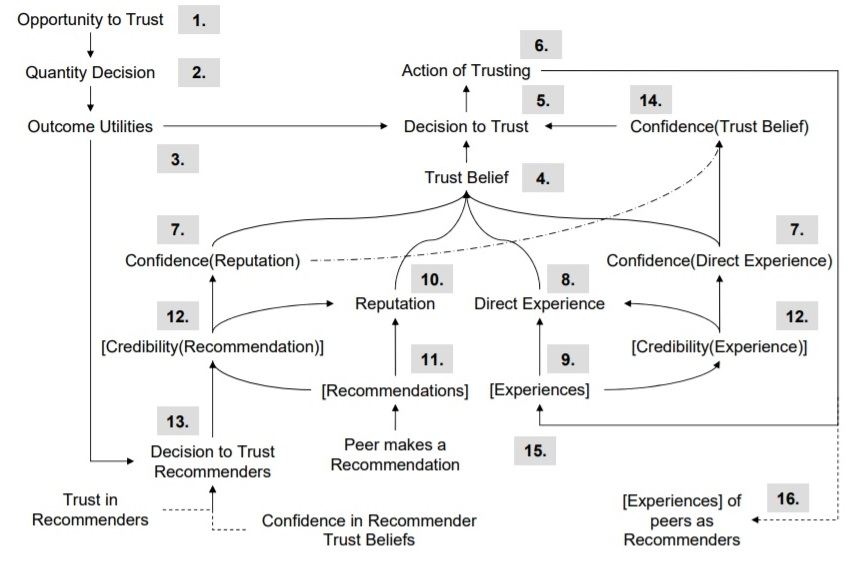
\includegraphics[width=0.85\textwidth]{006_team_4_agent_design/assets/JeremyPittTrustFramework.jpg}
    \caption{An illustration showing the formal model of the Trust Framework. \cite{JeremyPittSlides}}
    \label{fig:TrustFramework}
\end{figure}

The trust score acted as an element of symbiosis between the learning-based evolutionary algorithm that the agent was originally employed with and a self-organising strategy. Additionally, it allowed the agent to improve on it's relatively static structure to become more dynamic so as to adapt to the changes in it's surrounding environment. This was advantageous as the agent was able to use its pre-defined metrics in tandem with trust score and cravings to adapt within the tower depending on its social construction of reality. The trust score enacted the formal model (as shown in \Cref{fig:TrustFramework}) of a trust framework whereby the opportunity to trust is employed through communication and action, whilst the quantity decision is made through every individual agent strategy. Through local trust based modelling of a global trust score, the agent is able to implement the outcome utilities portion of the trust framework.

\section{Experimentation and Results}

\subsection{Baseline Comparisons}
In order to evaluate the performance of the agent, it was compared to two baselines - the default agent and the random agent. The time taken for the system to stabilise (\emph{i.e.,} time taken for the agents to organise into a structure that led to no future deaths) into a viable social order was measured. Tests with homogeneous populations of Team 4 agents, default agents and random agents were conducted, which highlighted that the two baselines never stabilised, whilst the Team 4 agent did. This was evident from \Cref{fig:baselinecomps} which showed the number of deaths for the Team 4 agents eventually stagnating however, this did not occur for the other two agent types. This was because the agent was able to build a trustworthy local perception which resulted in a positive outlook of the environment, allowing all agents to tend towards selflessness. This selfless behaviour enacted utilitarianism as the agents were able to maximise the average food left on the platform after a day had passed, ensuring that there was no wastefulness, whilst the overall population was still able to survive. 

\begin{figure}[htb]%
    \centering
    \subfloat[\centering Random Agent ]{{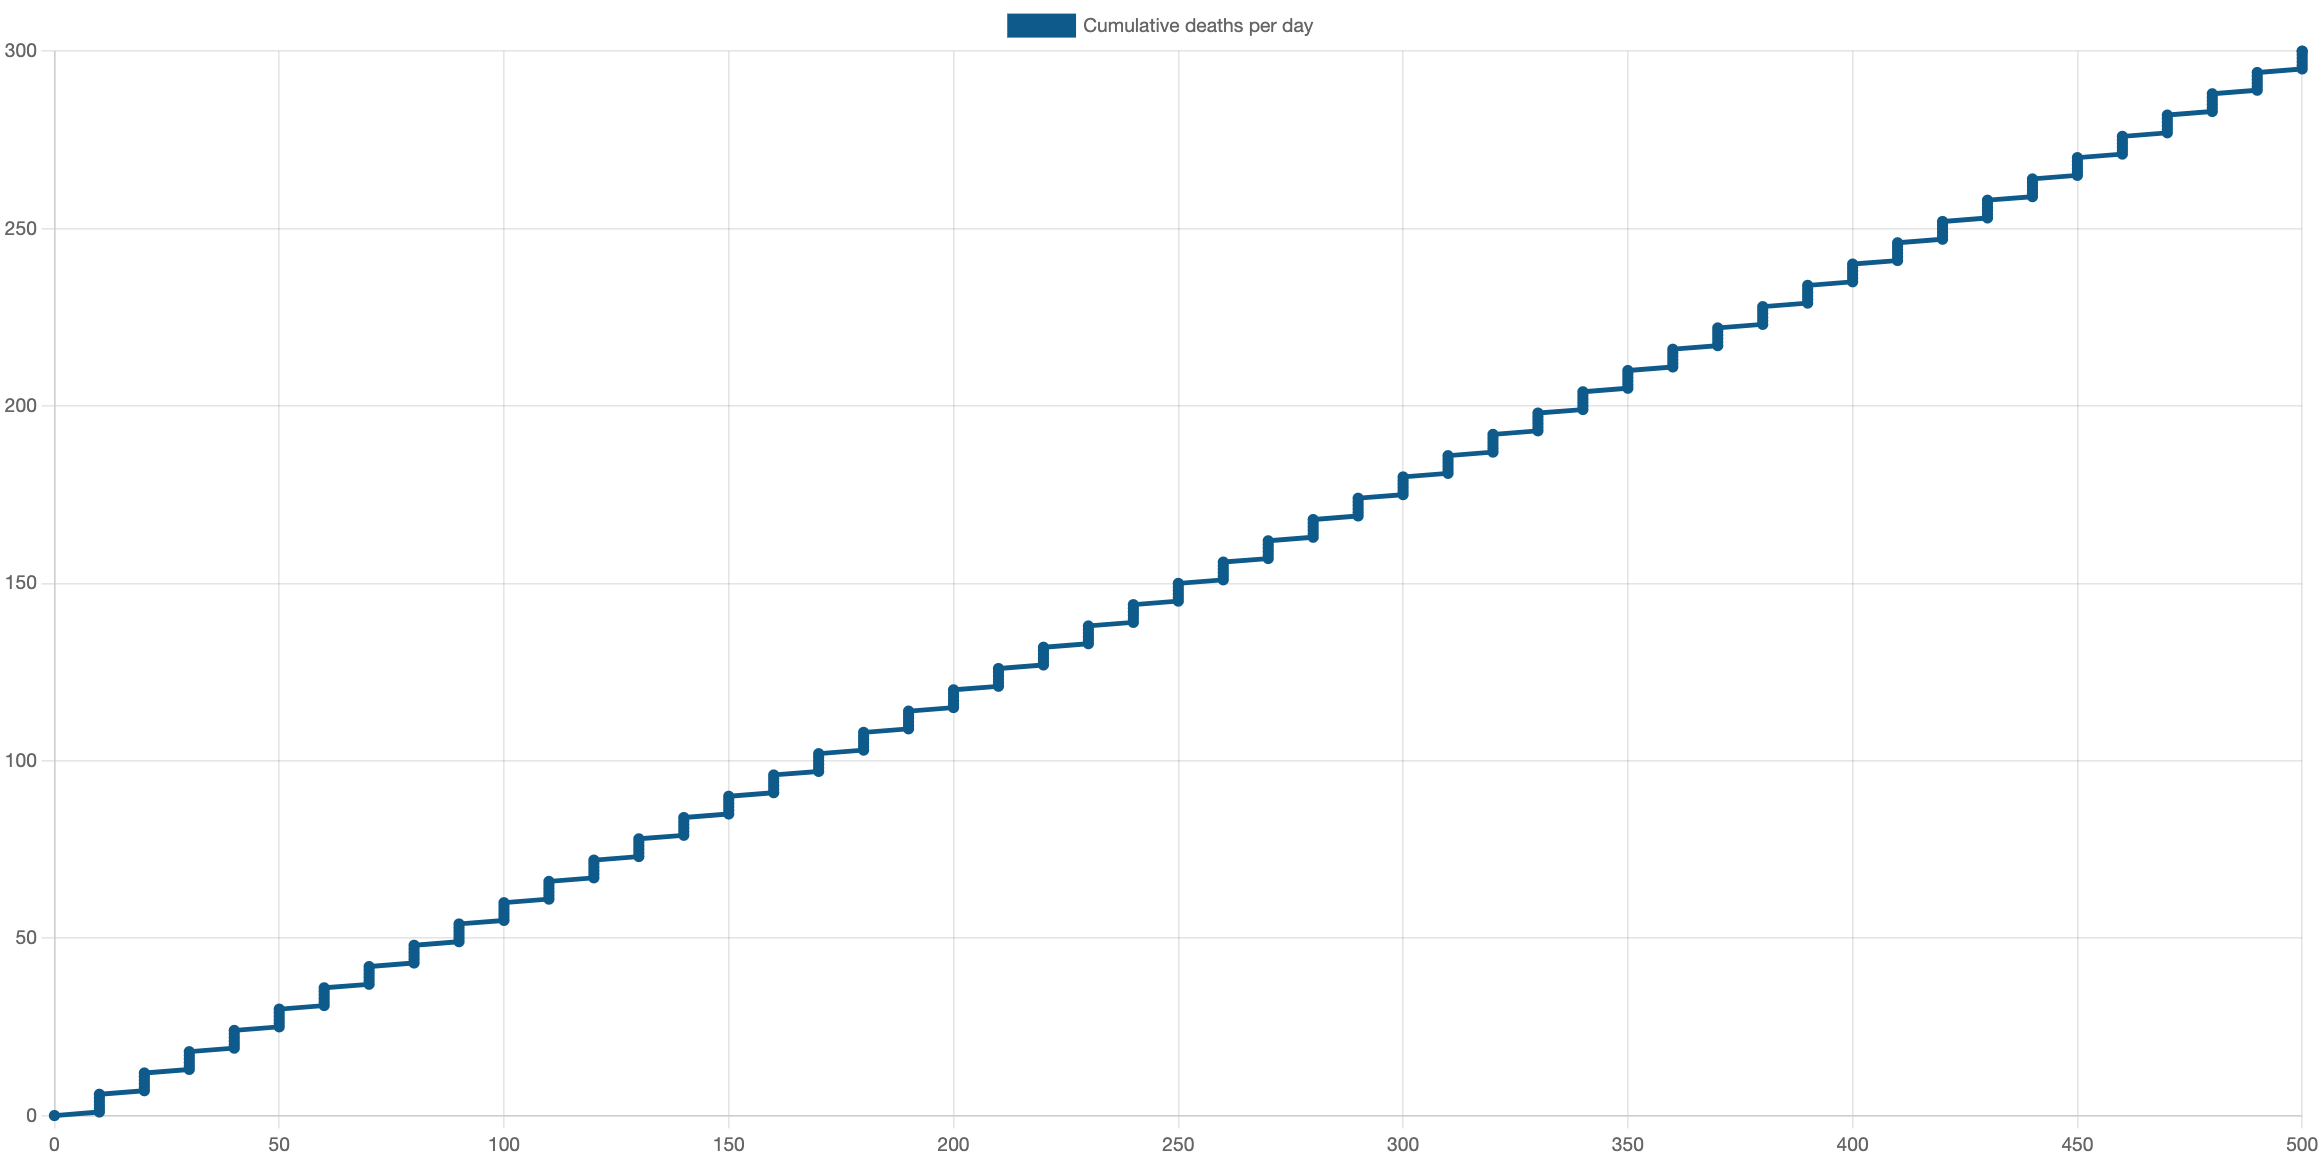
\includegraphics[width=0.4\linewidth]{006_team_4_agent_design/assets/unstabledefault.png}}}%
    \qquad
    \subfloat[\centering Default Agent ]{{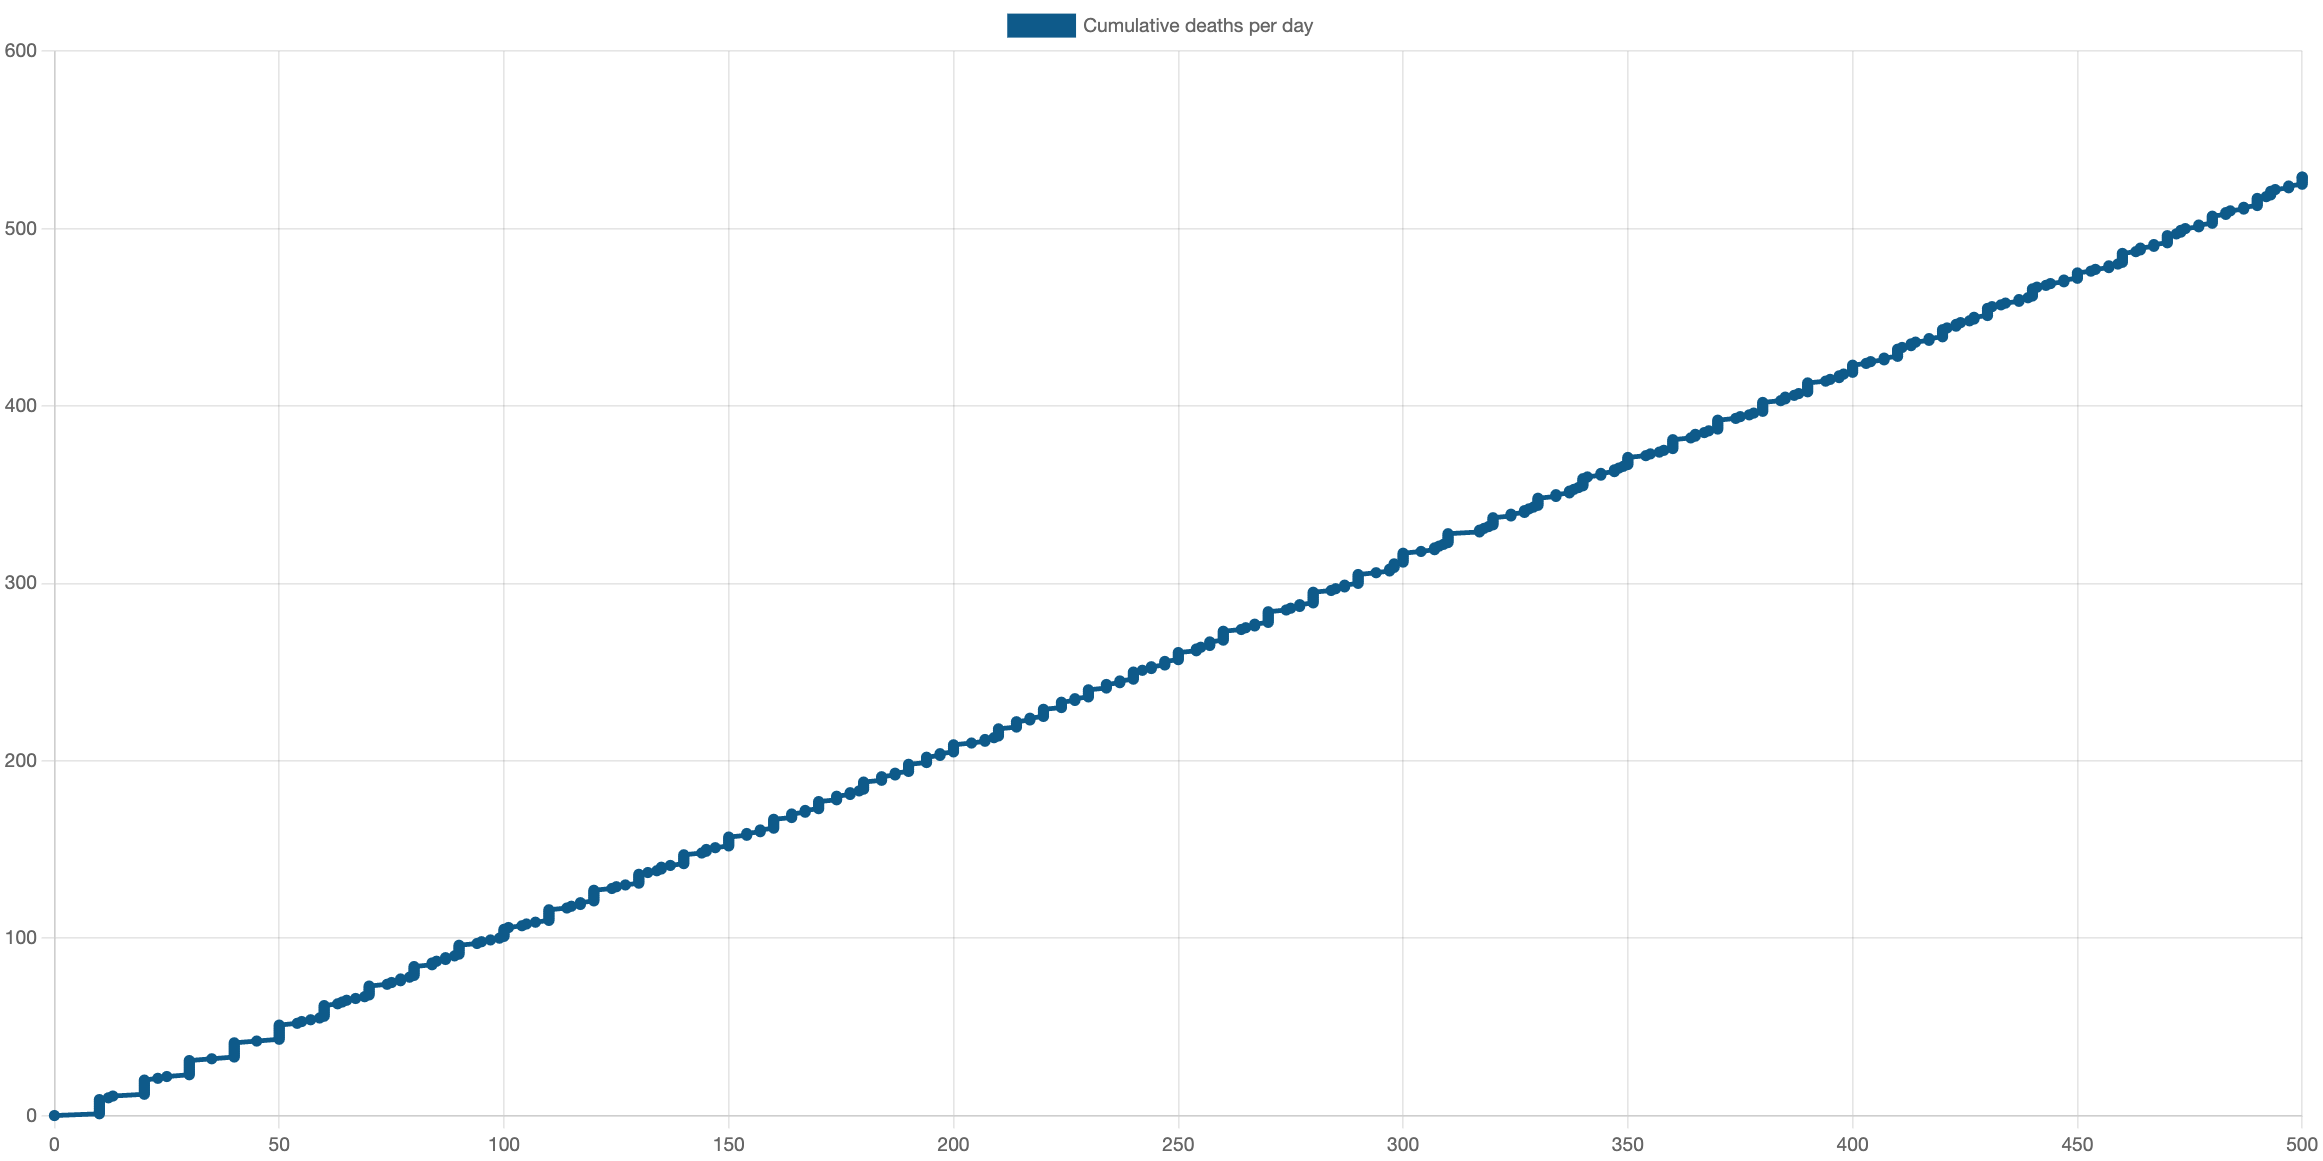
\includegraphics[width=0.4\linewidth]{006_team_4_agent_design/assets/unstablerandom.png}}}%
    \qquad
    \subfloat[\centering Team 4 Agent]{{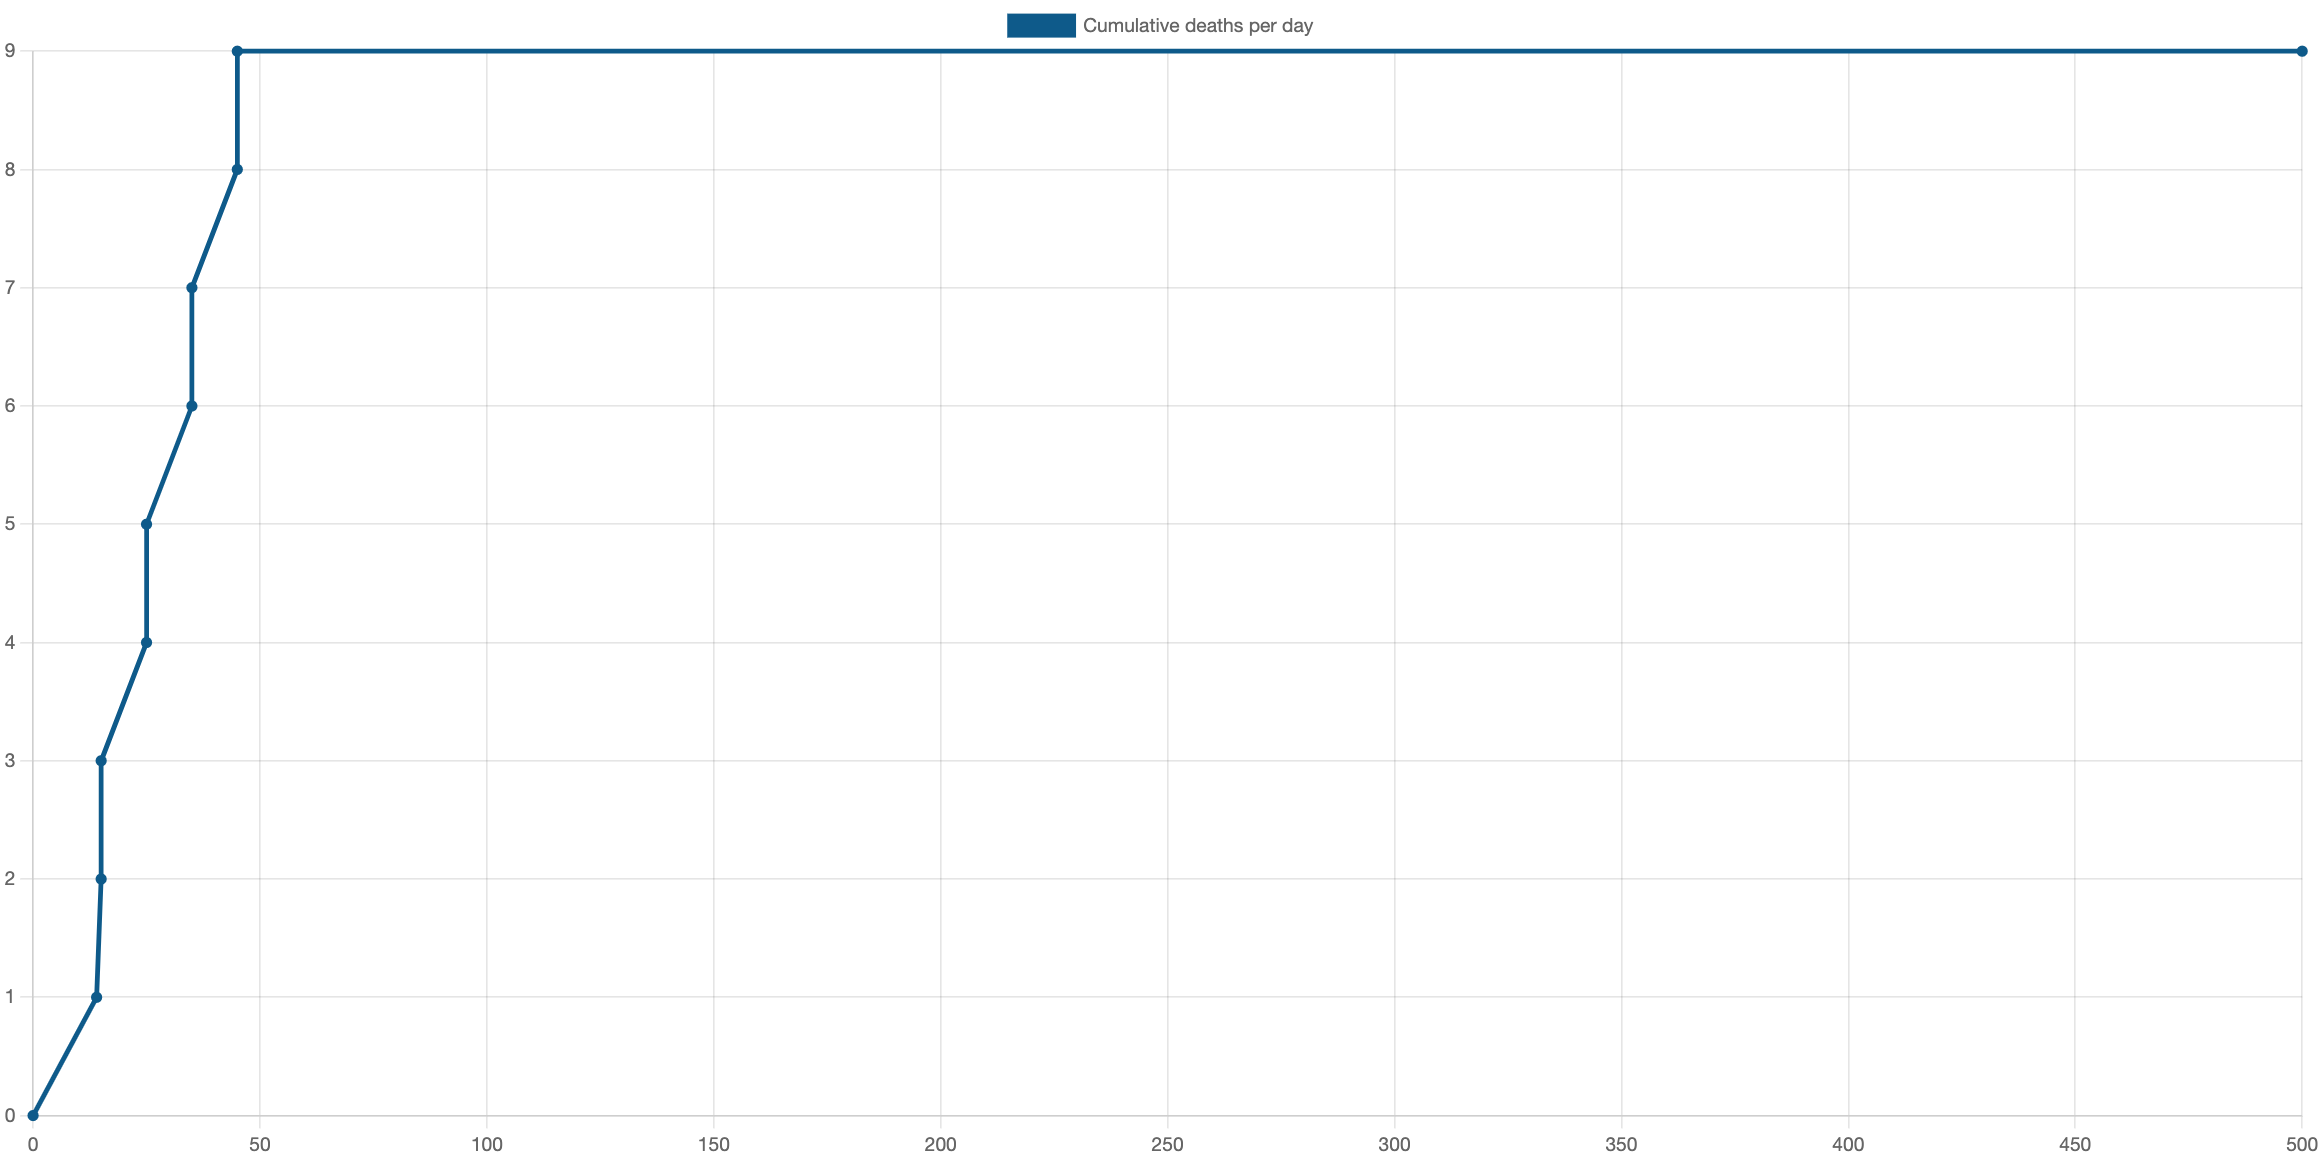
\includegraphics[width=0.4\linewidth]{006_team_4_agent_design/assets/stableus.png}}}%
    \caption{Graphs showing stabilisation times for various homogeneous populations of agents in the tower.}%
    \label{fig:baselinecomps}%
\end{figure}

\subsection{Stabilisation Times}

\subsubsection{Effect of Reshuffle Period}
\Cref{tab:reshuffleStabilisationTimes} shows the time taken for a system to stabilise with different numbers of reshuffle days. With longer reshuffle days, it took longer to stabilise as there were fewer opportunities for the agents to communicate with one another. This was the case since communications only occurred with a limited number of floors above and below the agent resulting in the agent only being able to create a limited view of its environment without reshuffling. 

\begin{table}[htb]
    \centering
    \begin{tabular}{|c|c|c|}
    \hline
    Reshuffle Days & Deaths & Days to Stabilise\\
        \hline
        \hline
        7 & 0 & 0 \\
        \hline
        25 & 4 & 24 \\
        \hline
        50 & 10 & 58 \\
        \hline
        100 & 18 & 94 \\
        \hline
    \end{tabular}
    \caption{Table showing stabilisation time for various reshuffle periods with 16 Team 4 agents.}
    \label{tab:reshuffleStabilisationTimes}
\end{table}

\subsubsection{Effect of Food Scarcity}
\Cref{tab:scarcityStabilisationTimes} shows the time taken for a system to stabilise with different levels of food scarcity. This scarcity was measured in amount of food per agent, meaning this value could decrease with both the food on the platform or number of agents in the tower. With more scarcity, the system took longer to stabilise since food became a more sought after resource, resulting in more conflict through competition over the shared resource which requires a longer time period for dispute resolution. When there was total scarcity of food, the system did not stabilise which was expected because there was simply not enough food for the agents to survive. With total abundance, the agents never die and form a stable system from the very beginning.

\begin{table}[htb]
    \centering
    \begin{tabular}{|c|c|c|}
    \hline
    Food Scarcity (food per agent) & Deaths & Days To Stabilise  \\
        \hline
        \hline
        Total Scarcity ($<$3) & $>$402 & does not stabilise \\
        \hline
        Satisfice (=3) & 27 & 167 \\
        \hline
        Total Abundance ($>$5) & 0 & 0 \\
        \hline
    \end{tabular}
    \caption{Table showing stabilisation time for various levels of food scarcity, reshuffling every 25 days, 500 days in total.}
    \label{tab:scarcityStabilisationTimes}
\end{table}

\subsubsection{Effect of Random and Selfish Agents}

A random agent was defined as an agent that eats random amounts of food on any given day. A selfish agent was defined as an agent that eats the amount of food it needs to remain at full HP. It was interesting to note the effect of each agent on homogeneous populations of Team 4 agents, and how many of them it took to destabilise the system.

\Cref{fig:selfishagentcomps} and \Cref{fig:randomagentcomps} show the behaviour of Team 4 agents with selfish and random agents respectively. In both instances, a similar trend was noticed; there were periods of stability but the system was disrupted to an unstable state soon after. Instances with the random agent were explained by the fact that it could not communicate with other agents and therefore no meaningful relationships could be created. Hence, even if stability was achieved through the communication between Team 4 agents, the unpredictable behaviour of the random agent quickly disrupted this. 
\newline
With the selfish agent, despite communication being present, Team 4 agents became selfish themselves due to distrust and a lack of communication from selfish parties. This meant both agent types acted in their own self interests causing the system to destabilise and the number of deaths increase.

\begin{figure}[htb]%
    \centering
    \subfloat[\centering 8 Team 4 agents with one selfish agent ]{{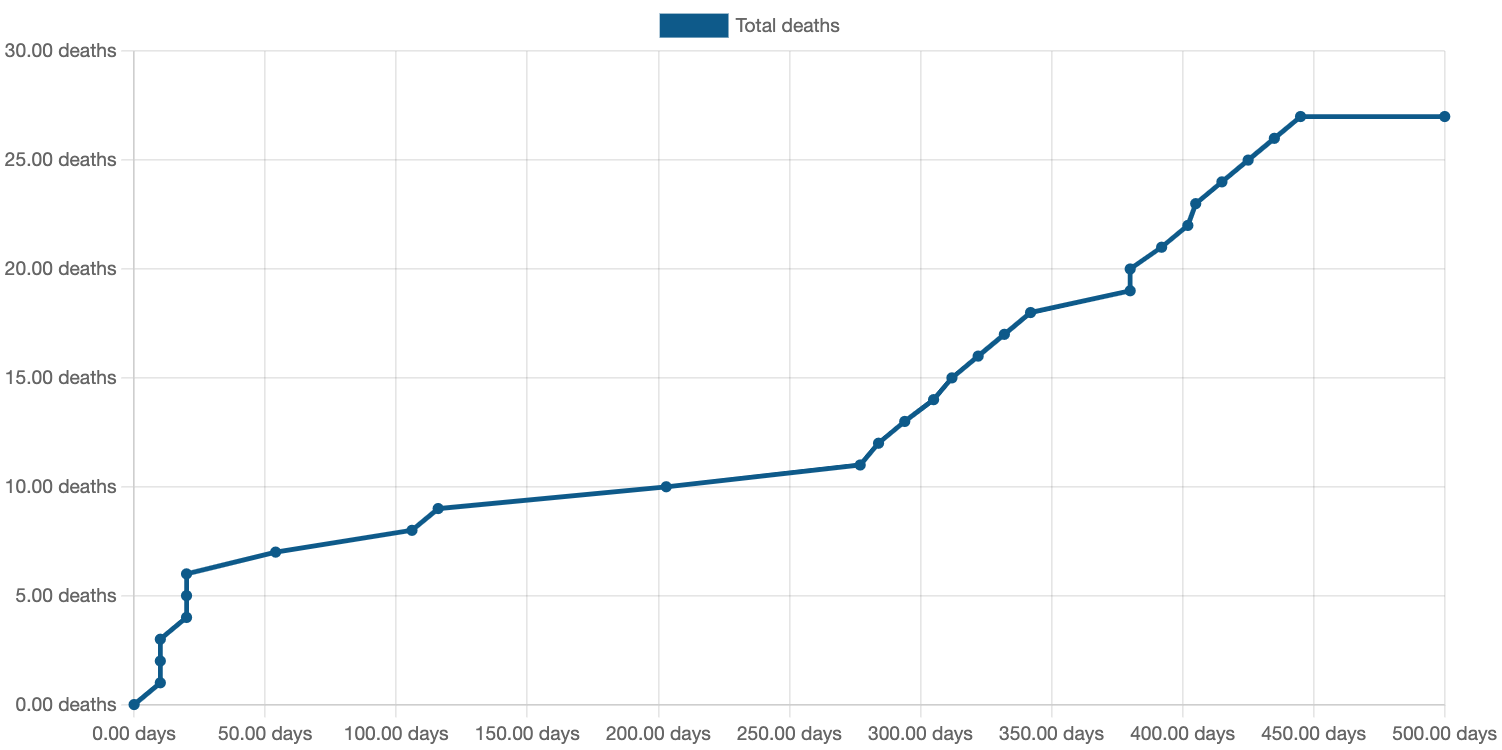
\includegraphics[width=0.45\linewidth]{006_team_4_agent_design/assets/selfishRuns/oneOtherSelfish.png}}}%
    \qquad
    \subfloat[\centering 8 Team 4 agents with two selfish agents ]{{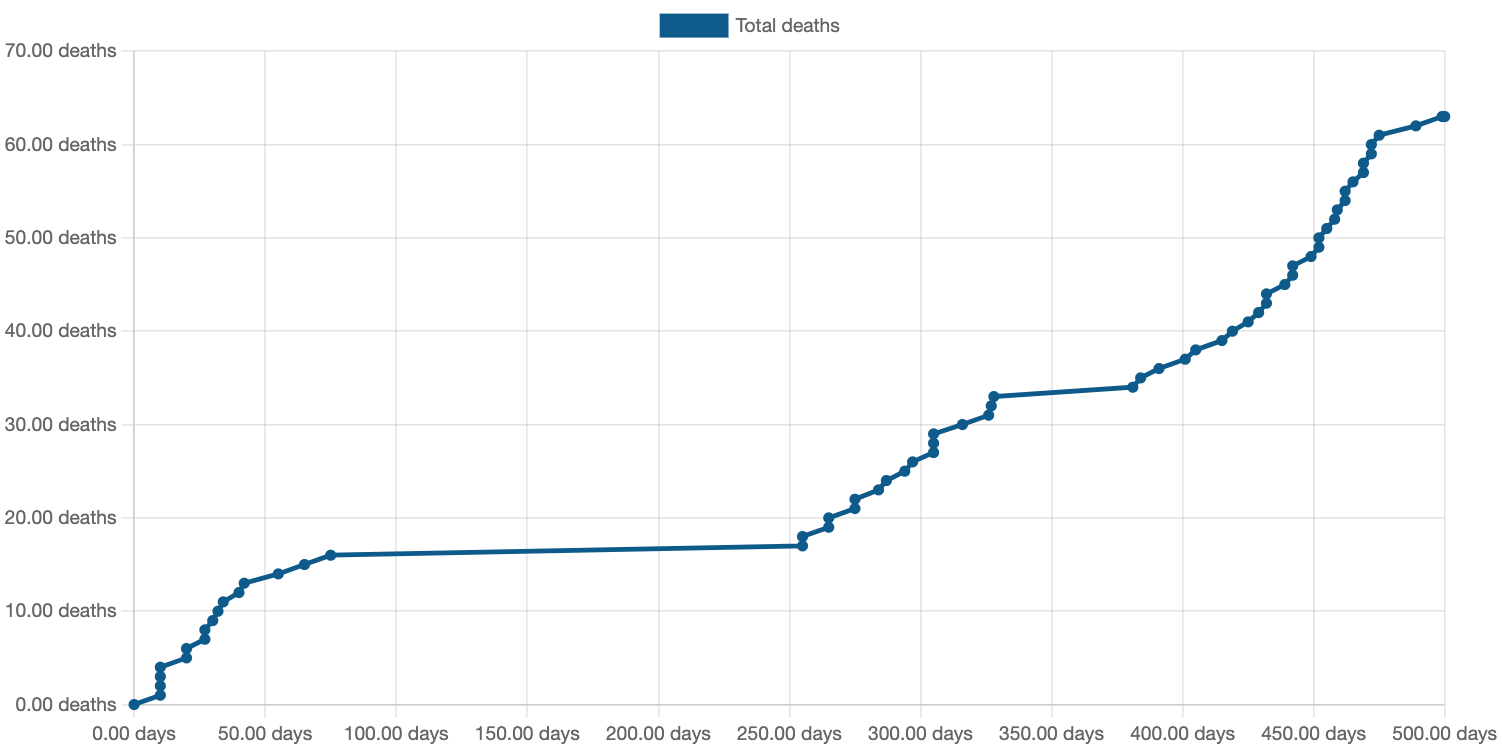
\includegraphics[width=0.45\linewidth]{006_team_4_agent_design/assets/selfishRuns/twoOtherSelfish.png}}}%
    \caption{Impact of selfish agents on system stability}%
    \label{fig:selfishagentcomps}%
\end{figure}

\begin{figure}[htb]%
    \centering
    \subfloat[\centering 8 Team 4 agents with one random agent ]{{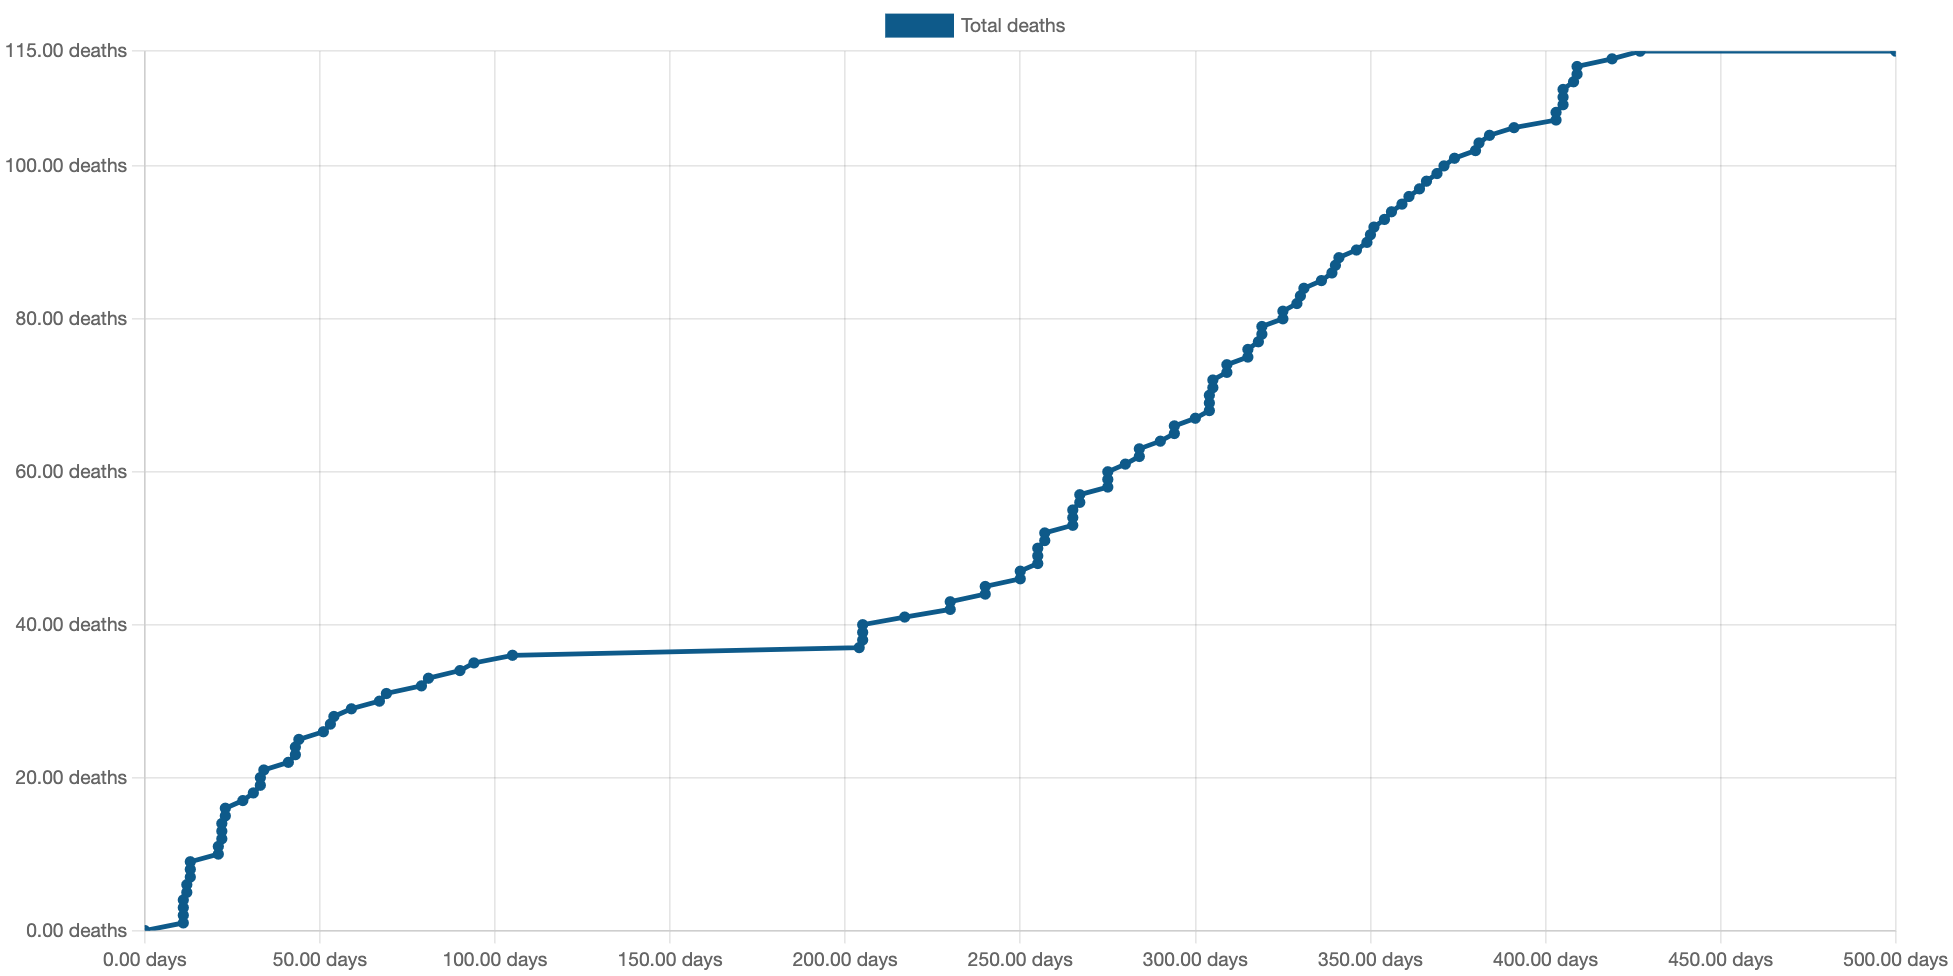
\includegraphics[width=0.45\linewidth]{006_team_4_agent_design/assets/randomRuns/oneOtherRandom.png}}}%
    \qquad
    \subfloat[\centering 8 Team 4 agents with two random agents ]{{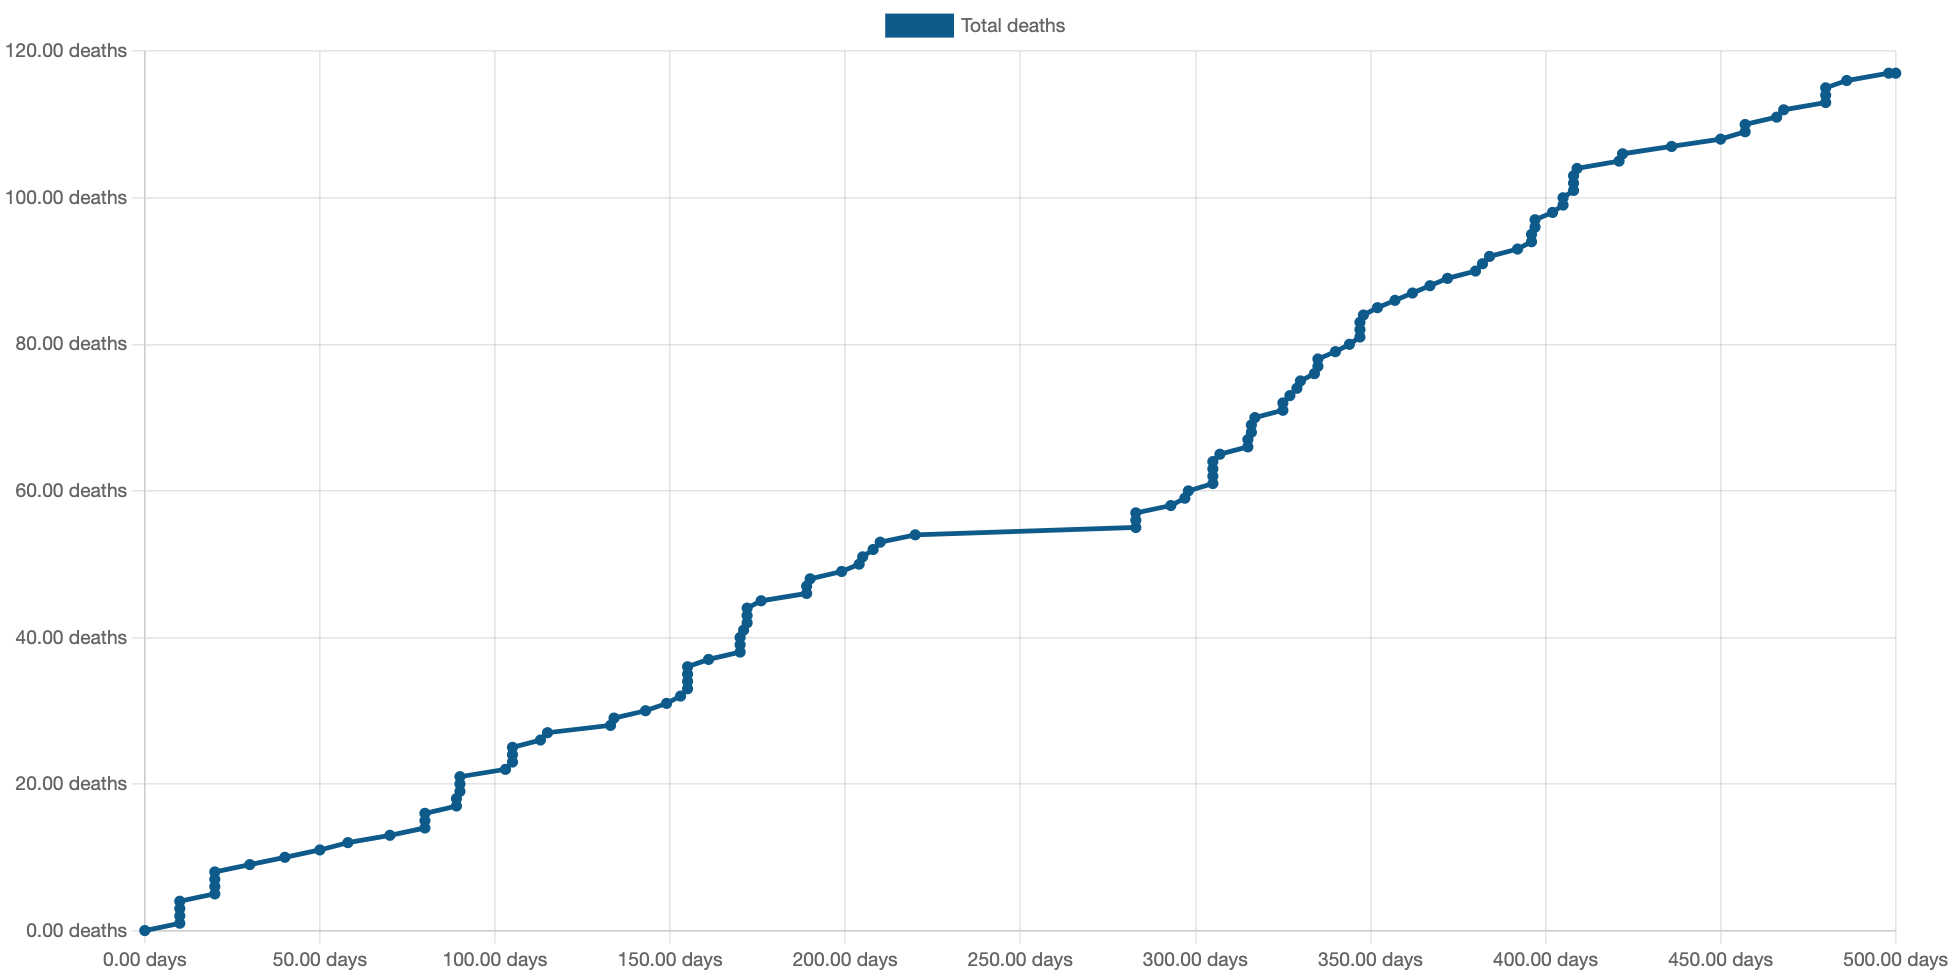
\includegraphics[width=0.45\linewidth]{006_team_4_agent_design/assets/randomRuns/twoOtherRandom.png}}}%
    \caption{Impact of random agents on system stability.}%
    \label{fig:randomagentcomps}%
\end{figure}

Overall, it can be said that the strategy of our evolutionary agent was very fragile and was easily effected by other more disruptive strategies.

\subsection{Communications and Interactions}

\subsubsection{Overview of Communications}
\Cref{fig:commsChart} shows the communications between agents in the tower on a particular run. A variety of messages were passed around, with the colours representing a particular message type. Theoretically, if the evolutionary agent had meaningful communications with other cultures, it should have been able to coexist with them.

\begin{figure}[htb]
    \centering
    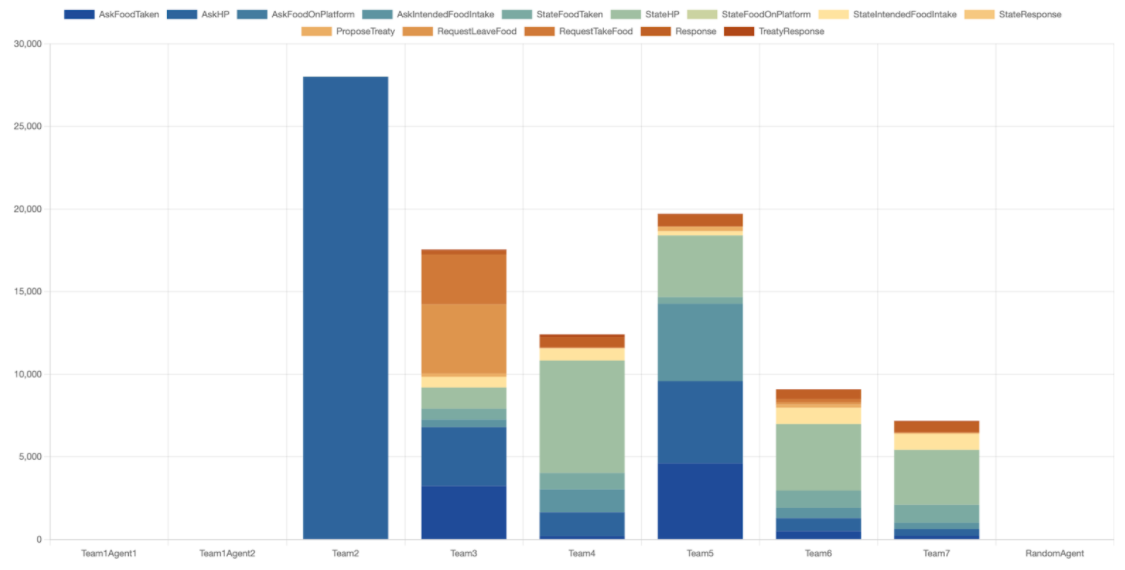
\includegraphics[width=0.85\textwidth]{006_team_4_agent_design/assets/communications_chart.png}
    \caption{A bar graph illustrating the various communications between agents.}
    \label{fig:commsChart}
\end{figure}

\subsubsection{Subsequent Compatibility with Other Cultures}
\Cref{tab:agentCompatibility} shows the compatibility of the evolutionary agent culture compared to the various cultures of other implemented agents. It is clear Teams 3, 5 and 7 were very compatible with the evolutionary agent as a result of fair communication allowing the agents to form a viable social structure, resulting in 0 deaths after a certain period of time. Teams 5 and 7 were particularly fast in forming this structure, suggesting that communication between the two were very efficient.

\begin{table}[htb]
    \centering
    \begin{tabular}{|p{5em}|p{5em}|p{5em}|p{5em}|p{9em}|}
    \hline
        Other Agent Team & Number of Deaths & Our Deaths & Other Deaths & Compatible? (stabilises within 500 days) \\
         \hline
         \hline
        2 & 222 & 146 & 76 & No \\
         \hline
        3 & 82 & 59 & 23 & Yes \\
         \hline
        5 & 2 & 1 & 1 & Yes \\
         \hline
        6 & 259 & 161 & 98 & No \\
         \hline
        7 & 4 & 0 & 4 & Yes \\
         \hline
    \end{tabular}
    \caption{Table showing compatibility of various agent cultures with the evolutionary agent.}
    \label{tab:agentCompatibility}
\end{table}

In contrast, other agent types did not have as fortunate an outcome, and they were never really able to find a system that led to everyone surviving. It can be inferred subsequently that message passing and treaties themselves were not sufficient methods in these cases, and those agents' ideologies differed from the evolutionary agents by a great degree.

\section{Future Work}
Though the agent performed quite well in a homogeneous system, future work can be conducted to try and improve the agent's strategy. Some of the avenues for exploration are outlined below:

\begin{itemize}
    \item Making agent more resilient to other disruptive cultures such as random agents 
    \item Making the symbiosis of trust score and evolution more prevalent by including communications in the evolution process
    \item Including more genotypes to learn during the evolutionary process
    \item Including more complex treaty implementations to enforce Team 4 agent strategy.
\end{itemize}
\chapter{Team 5 Agent Design}\label{team_5_agent_design}

The Team 5 agent operates on the basis that upon entering the tower, the need to ensure its own survival is its only aim and therefore the agent should maximise its own HP whenever given the opportunity to do so. When there is not enough food to fully satisfy all agents, the agent alters its behaviour to best increase its long-term survival.

This situation can be thought of as a `hawk-dove' game where it is beneficial for all agents to take less food but any single agent who does so is worse off if no other agents follow suit. Communication is key to breaking out of this situation. This agent will attempt to establish relationships with surrounding agents -- the agent has parameters to judge other agents and also attempts to learn about the tower -- and encourage behaviours that benefit the overall tower utility.

However, the agent will also be influneced by the behaviour of agents around it: if other agents are selfish then it will also be selfish. This can be thought of as a `tit-for-tat' strategy, but with enough HP, agents will be willing to `make the first move', with the insurance that if others do not follow then they have some buffer time to re-establish their own selfish behaviour.

An agent will maintain a low HP only if it is confident that other agents will allow it to survive by leaving enough food, through the signing of treaties to build trust. A tower that consists solely of Team 5 agents would require those at the top to be willing to decrease their own short-term satisfaction in order to give the best chance of survival for all agents, and trust others to do the same upon reshuffling.

Section \ref{sec:team5-overview} provides an overview of the agent's parameters and strategy, Section \ref{sec:team5-messaging} describes the agent's communication strategy, Section \ref{sec:team5-memory} describes how the agent stores its social network and how it judges other agents, and Section \ref{sec:team5-treaties} describes how the Team 5 agent utilises treaties. Finally, Section \ref{sec:team5-experimentation} contains analysis of this agent and how it performs in a Tower consisting of itself alone and together with other agent types and Section \ref{sec:team5-conclusion} provides summarising remarks regarding the implementation of this agent type.

\section{Agent Overview}
\label{sec:team5-overview}

\ToDo{Give better description of Run function}

The strategy employed by this agent aims to maximise its chances of survival while also considering those who have helped the agent in the past.

At the beginning of each day, the agent's `personality' is updated using various parameters stored from previous days. These personality parameters are shown in Table \ref{tab:team5-personality}.

\begin{table}
    \centering
\begin{tabular}%
    {| >{\raggedleft\arraybackslash}p{0.25\linewidth} | %
    >{\raggedright\arraybackslash}p{0.65\linewidth} | %
    }
    \hline
    Selfishness          & Ranges from 0 to 10. Determines how much the agent will act for their own survival as opposed to the best interests of the surrounding agents\\
    \hline
    Last Meal            & How much the agent ate in their last meal\\
    \hline
    Days Since Last Meal & How many days since the agent last ate\\
    \hline
    % HP After Eating      & \\
    % \hline
    Aim HP               & Defines the goal HP the agent would like to reach at the end of the day\\
    \hline
    Attempt Food         & The amount of food the agent will attempt to take from the platform\\
    \hline
    Messaging Counter    & Determines which message type to send to which floor \\
    \hline
    % Treaty Send Counter  & \\
    % \hline
    % Attempt To Eat       & \\
    % \hline
    Leadership           & A threshold value required for the agent to propose treaties\\
    \hline
    Social Memory        & Stores the information the agent learns about other agents, as well as its opinion of them (see Table \ref{tab:team5-memory})\\
    \hline
    Surrounding Agents   & A list of the agent's neighbours\\
    \hline
\end{tabular}
\caption{The personality parameters of Team 5's agent}
\label{tab:team5-personality}
\end{table}

At the start of each tick, the agent checks to see if it has received any messages and if so, will respond to these\footnote{Note that an agent can receive and respond to only one message per tick.}. The agent then sends out messages to other agents. The mechanism for messaging is described in Section \ref{sec:team5-messaging}.

\section{Messaging}\label{sec:team5-messaging}
Collaboration between different agents operating in a system requires communication. The motivation for messaging is to improve the agent's understanding of its surroundings, enable building of mutually beneficial relationships, and introduce collaboration and argeement between parties.

\subsection*{Strategy}\label{sec:team5-messaging-strategy}
The agent's approach to messaging is to adopt a ``passive observer'' role focussed on gathering information about other agents to organise itself with these agents in the tower. With more information at its disposal, the agent can make more informed decisions to balance its own individual utility with the collective utility of the agents in the tower.

\ToDo{choose whether to say 12 or 8 ticks to send all messages}\\
\ToDo{choose whether to include intended food intake in messages}\\
The agent sends three types of messages to each of the agents residing one or two floors above and below its own floor; it therefore takes 12 ticks to send all of its messages. These messages ask for the HP, intended food intake, and actual food intake of other agents. The decision of which message type to send to which floor is controlled by the Messaging Counter described in Table \ref{tab:team5-personality}. This counter is incremented each tick, and reset either every 25 ticks or at the end of each day, whichever comes first. This ensures that the agent is requesting up-to-date information regularly for use in its decision making.

The order of sent messages is:
\begin{enumerate}
    \item Ask for an agent's HP
    \item Ask for an agent's previous food intake
    % \item Ask for an agent's intended food intake
\end{enumerate}
The Team 5 agent first targets the agent immediately below it, then the agent immediately above, then two floors below, and finally the agent two floors above.

\section{Social Memory}\label{sec:team5-memory}
The agent stores the information gained from communication in its `memory': the information stored by this data structure is shown in Table \ref{tab:team5-memory}.

\begin{table}
    \centering
    \begin{tabular}%
        {| >{\raggedleft\arraybackslash}p{0.25\linewidth} | %
        >{\raggedright\arraybackslash}p{0.65\linewidth} | %
        }
        \hline
        Agent ID & An agent's unique ID\\
        \hline
        Agent HP & The agent's HP level\\
        \hline
        Food Taken & The amount of food the agent last took\\
        % \hline
        % Intended Food Intake & The amount of food the agent intends to take\\
        \hline
        Favour & The Team 5 agent's opinion of this agent\\
        \hline
        Days Since Last Seen & The number of days since the last message from this agent\\
        \hline
    \end{tabular}
    \caption{Team 5 Agent Memory}
    \label{tab:team5-memory}
\end{table}

This memory allows the agent to construct a social network of agents in the tower and evaluate others based on these parameters. This consequently leads to the idea of favour, a metric the Team 5 agent uses to judge other agents. If more than five days have passed since the agent's last interaction with someone, then the memory of that agent is reset. This prevents the agent from using out-of-date information in its calculation and also allows for the removal of dead agents from its memory.

\subsection*{Favour}\label{sec:team5-favour}
The favour metric quantifies the agent's opinion of others in the tower. It is bounded between 0 and 10, and in a single tick can either increase by 1, decrease by 3, or stay the same:

\begin{align*}
    \texttt{hpScoreOther} &= -1 \times \frac{\texttt{otherHP}^{1.7} \times \texttt{foodTaken}^{1.3}}{\texttt{maxHP}^3}\\
    \texttt{hpScoreSelf} &= \frac{\texttt{ownHP}^{1.7}\times\texttt{ownAttemptFood}^{1.3}}{\texttt{maxHP}^3}\\
    \texttt{judgement} &= 100 \times (\texttt{hpScoreOther} + \texttt{hpScoreSelf})\\
    \texttt{unboundedFavour} &= \begin{cases}
        \texttt{originalFavour} + 1, \quad\hfill \texttt{judgement} &> 0.075\\
        \texttt{originalFavour} + \max{\left(\frac{\texttt{judgement}}{2}, -3\right)}, \quad\hfill\texttt{judgement} &< -2
    \end{cases}\\
    \texttt{favour} &= \begin{cases}
        0, \quad\hfill \texttt{unboundedFavour} &< 0\\
        \texttt{unboundedFavour}, \quad 0 \leq \texttt{unboundedFavour} &\leq 10\\
        10, \quad\hfill \texttt{unboundedFavour} &> 10
    \end{cases}\\
\end{align*}

Measuring favour allows the agent to act accordingly to how other agents are behaving around it, while taking on a passive conformist approach to decision making. If the agent views others around it more favourably, then it eats less food and aims for a lower HP in hopes of improving collective utility. The agent is also more likely to propose treaties to, and accept treaties from, highly favoured agents.

For agents which have low favour, the Team 5 agent maintains its passiveness and does not ``punish'' them by, for example, taking more food than is necessary. The effect of ``punishing'' an agent propagates to all floors below the agent and is therefore not deemed an appropriate course of action. Instead, the agent strives to behave positively if surrounding agents also demonstrate positive behaviour.

It should also be noted that while the Team 5 agent computes favour for agents both above and below its floor, a positive favour value for agents above is helpful to that agent only if they are moved to a floor below the Team 5 agent following a reshuffle: this is because there is no way to reward the behaviour of an agent above you in the tower.

\section{Treaties}\label{sec:team5-treaties}
The Team 5 agent's treaty strategy consists of three main parts:
\begin{enumerate}
    \item Deciding whether to accept or reject proposed treaties
    \item When to propose a treaty
    \item What to propose as a treaty
\end{enumerate}

\subsection*{Responding to Proposed Treaties}\label{sec:team5-treaties-response}
A proposed treaty is always rejected if:
\begin{itemize}
    \item It conflicts with any other active treaties. A treaty is considered to conflict with another treaty if they could ever cause the agent to incompatible actions (for example, an agent cannot leave more than five units of food and fewer than four units of food at the same time).
    \item It is badly formed. For example, a treaty which requires the agent to leave more than 100\% of the food on the platform is badly formed.
    \item \ToDo{Check this one} It requires agents to leave less than a certain amount of food on the platform, as this is never advantageous to the tower as a whole.
    \item \ToDo{Check this one} It requires the agent to leave an exact amount of food on the platform, as this would result ina ll but one of the agents signed up to the treaty to take no food each day.
    \item It makes a request based on low HP, low amounts of food on the platform, or a low floor, as in these conditions the agent will already be desperate for survival, so will not want to be further constrained by a treaty.
    \item \ToDo{Check this one} It makes a request based on HP where the threshold is within the ``weak'' or ``critical'' HP bands, as this means the agent could become critical or die as a result of following the treaty.
    \item \ToDo{Check this one} It would require the agent to take less food than is required to avoid entering the ``critical'' HP band.
\end{itemize}
If the treaty does not meet any of the above conditions, the \texttt{decision} value is then computed as:
\[\texttt{decision} = 6 - \texttt{selfishness} + \texttt{proposerFavour} - \frac{\texttt{treatyDuration}}{3}\]

This calculation is based on the following considerations:
\begin{itemize}
    \item Selfish agents will always be less likely to sign treaties
    \item The proposing agent is more likely to be trusted if the receiving agent views them more favourably
    \item Longer treaties are viewed more negatively because factors such as the receiving agent's opinion of the proposer and the agent's selfishness can change over time, meaning the same treaty could be viewed less favourably in future. Therefore, the agent should avoid constraining its actions to satisfy an agent of which it has a negative opinion.
\end{itemize}

If the \texttt{decision} value is positive, the treaty is accepted.

\subsection*{Proposing Treaties}\label{sec:team5-treaties-proposal}
At the start of each day, the agent checks whether it has become a `leader': if it has, then the agent proposes a treaty. Whether an agent becomes a leader or not is based on:
\begin{itemize}
    \item The agent's selfishness: a selfish agent is less likely to propose treaties
    \item The agent's floor: agents higher up in the tower are more likely to propose treaties. This is because agents higher up in the tower have more access to food and therefore have more control over the food available to those below them. This control means these agents are in a better position to affect change.
    \item The agent's \texttt{leadership} threshold: this is randomly set during the agent's initialisation and those with a lower leadership threshold are more likely to become leaders.
\end{itemize}
The leadership value is calculated by:
\[ \texttt{leadership} = x - \texttt{selfishness} - \texttt{agentFloor}\]
The variable $x$ is a random number between 3 and 12, inclusive. If $leadership$ is greater than the agent's leadership threshold, then the agent becomes a leader and proposes a treaty.

The proposed treaty is always that agents whose HP is greater than or equal to a certain value should always leave 100\% of the food on the platform, and always lasts for five days. The threshold value for HP is calculated using Equation \ref{eq:team5-treaty-hp-threshold}. Note that in this equation, \texttt{WeakLevel} refers to the threshold between the ``critical'' and ``weak'' HP states.

\begin{equation}\label{eq:team5-treaty-hp-threshold}
    \texttt{hpThreshold} = \texttt{aimHP} - \frac{\texttt{aimHP} - \texttt{WeakLevel}}{10}\times\left(\texttt{leadership} - \texttt{leadershipThreshold}\right)
\end{equation}

\section{Experimentation}\label{sec:team5-experimentation}
This section focuses on how the agent's performance varies with changes in its environment.

\subsection*{Homogeneous Tower Experiments}
To evaluate the self-organisation abilities of the Team 5 agent, simulations were run with the agent in variations of a homogeneous tower (i.e. a tower that contains agents of only one type). The agent has been evaluated on three main metrics:
\begin{enumerate}
    \item The number of deaths
    \item The average utility
    \item Whether self-organisation was achieved.
\end{enumerate}
Self-organisation has been defined in this case to be when all agents take only what they need to survive and there are little to no deaths beyond a certain point in time.

\subsubsection*{Food Per Agent On Platform}
The baseline experiment for testing was to vary the amount of food per agent available on the platform; it was expected that having more food available would result in fewer deaths. In this experiment, simulations were run for 100 simulation days, with a reshuffle period of 7 days and 50 agents in the tower and repeated three times, with the average of these runs taken. Figure \ref{fig:team5-deaths-utility-food-per-agent} shows that the number of deaths decreases and average utility increases as we increase the amount of food available.

When the ratio of food to agent is greater than 9, the agents are able to self-organise within 100 days, and typically do so within 70 days. When food availability was less than this, the agents did not achieve self-organisation. However it was interesting to observe that more treaties were accepted than rejected. This shows that the agents recognise the need to self-organise and are willing to make attempts to do so. It is possible that they did not achieve self-organisation because agents died too quickly to reach agreements among enough agents for this to be successful.

\begin{figure} % Number of Deaths and Average Utility vs Available Food Per Agent
    \centering
    \begin{minipage}{0.6\textwidth}
        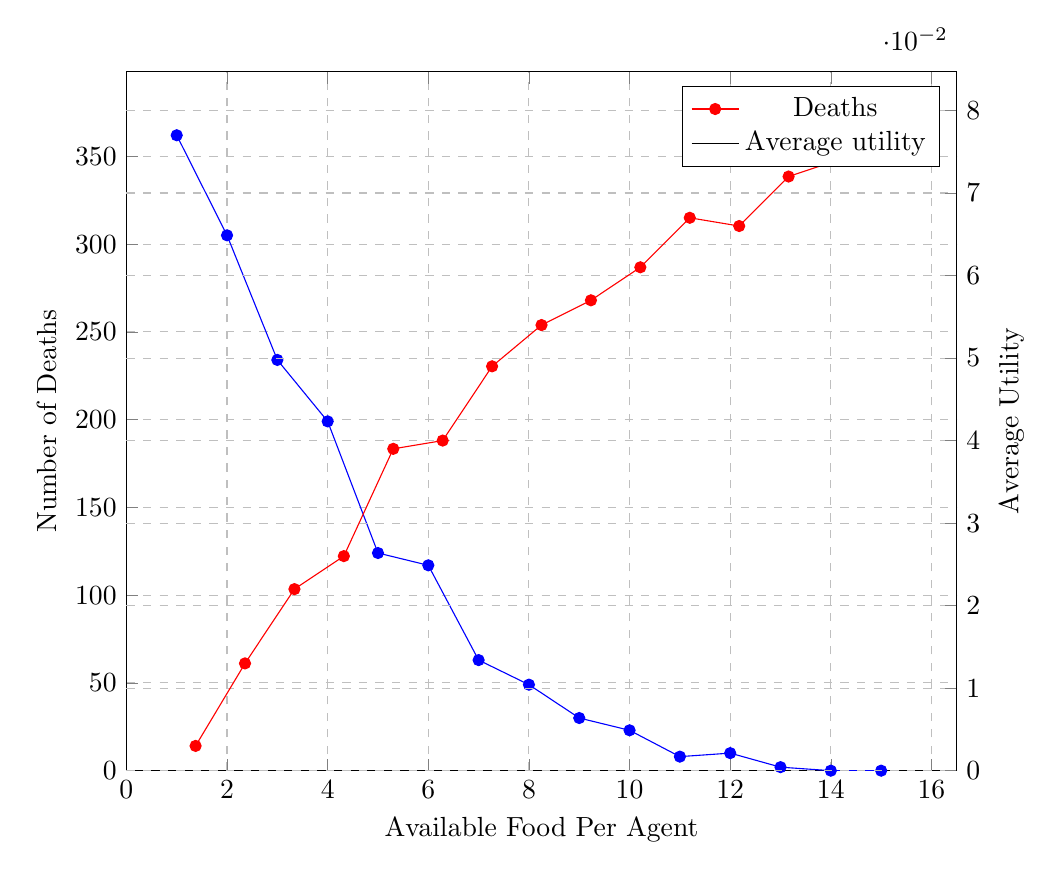
\begin{tikzpicture}
            \begin{axis}[
                width=\textwidth,
                axis y line*=left,
                ymin=0,
                xmin=0,
                xlabel=Available Food Per Agent,
                ylabel=Number of Deaths,
                ymajorgrids=true,
                xmajorgrids=true,
                grid style=dashed,
            ]
            \addplot[mark=*,blue]
                coordinates{
                    (15, 0)
                    (14, 0)
                    (13, 2)
                    (12, 10)
                    (11, 8)
                    (10, 23)
                    (9, 30)
                    (8, 49)
                    (7, 63)
                    (6, 117)
                    (5, 124)
                    (4, 199)
                    (3, 234)
                    (2, 305)
                    (1, 362)
                }; \label{leg:team5-food-per-agent-deaths}
            \end{axis}
            
            \begin{axis}[
                width=\textwidth,
              axis y line*=right,
              axis x line=none,
              ymin=0,
              ylabel=Average Utility,
              ymajorgrids=true,
              xmajorgrids=true,
              grid style=dashed,
            ]
            \addplot[mark=*,red]
                coordinates{
                    (15, 0.077)
                    (14, 0.074)
                    (13, 0.072)
                    (12, 0.066)
                    (11, 0.067)
                    (10, 0.061)
                    (9, 0.057)
                    (8, 0.054)
                    (7, 0.049)
                    (6, 0.04)
                    (5, 0.039)
                    (4, 0.026)
                    (3, 0.022)
                    (2, 0.013)
                    (1, 0.003)
                }; \label{leg:team5-food-per-agent-utility}
                \addlegendimage{/pgfplots/refstyle=leg:team5-food-per-agent-deaths}\addlegendentry{Deaths}
                \addlegendimage{/pgfplots/refstyle=leg:team5-food-per-agent-utility}\addlegendentry{Average utility}
            \end{axis}
            \end{tikzpicture}
    \end{minipage}
    \caption{Number of Deaths and Average Utility vs Available Food Per Agent}
    \label{fig:team5-deaths-utility-food-per-agent}
\end{figure}

\subsubsection*{Number of Agents}
Through experimenting with the Team 5 agent, it was found that the variable with the largest effect on the likelihood of self-organisation being achieved was the number of agents present in the tower. This is likely an effect of the agent strategy relying heavily on communicating and establishing relationships with other agents. Having more agents in the tower means that it takes longer to form opinions of every other agent, and the likelihood of being reshuffled next to other agents that you have already seen decreases as the number of agents increases.

After making this observation, it was decided that it would be interesting to investigate how long it takes for varying numbers of Team 5 agents to self-organise for a given amount of food available. Table \ref{tab:team5-exp-num-agents} shows the results of varying the number of agents in the tower, with the food per agent ratio set to 2.

\begin{table}
    \centering
    \begin{tabular}{|c|c|c|}
        \hline
        \textbf{Number of agents} & \textbf{Days to organise} & \textbf{Deaths before self-organisation}\\
        \hline
        $<$10 & 0 & 0 \\
        \hline
        15 & 80 & 46 \\
        \hline
        15 & 0 & 0 \\
        \hline
        17 & 0 & 0 \\
        \hline
        18 & 45 & 22\\
        \hline
        18 & 95 & 79 \\
        \hline
        20 & \multicolumn{2}{c|}{No organisation in 500 days}\\
        \hline
        20 & 242 & 226 \\
        \hline
        25 & \multicolumn{2}{c|}{No organisation in 700 days}\\
        \hline
        
    \end{tabular}
    \caption{The number of deaths and number of days required for Team 5 agents to self-organise}
    \label{tab:team5-exp-num-agents}
\end{table}

The results show that the length of time it takes for the agents to organise is very variable: randomness plays a large factor due to the many random variables present in the simulation, such as an agent's floor and its leadership threshold. For organisation to occur, agents who are more likely to become leaders need to become less selfish and be reshuffled high up in the tower. This will enable them to send treaties to surrounding agents. The surrounding agnets must view them favourably enoguh to accept the treaties they receive.

It was found that, with the food per agent ratio set to 2, there appeared to be a threshold value of approximately 18 agents were organisation was far less likely to occur within the early days of the tower. Further testing showed that this threshold increases with the amount of food available per agent. Figure \ref{fig:team5-20agents-2food} shows the results of a simulation where 20 agents managed to organised themselves.

\begin{figure}
    \centering
    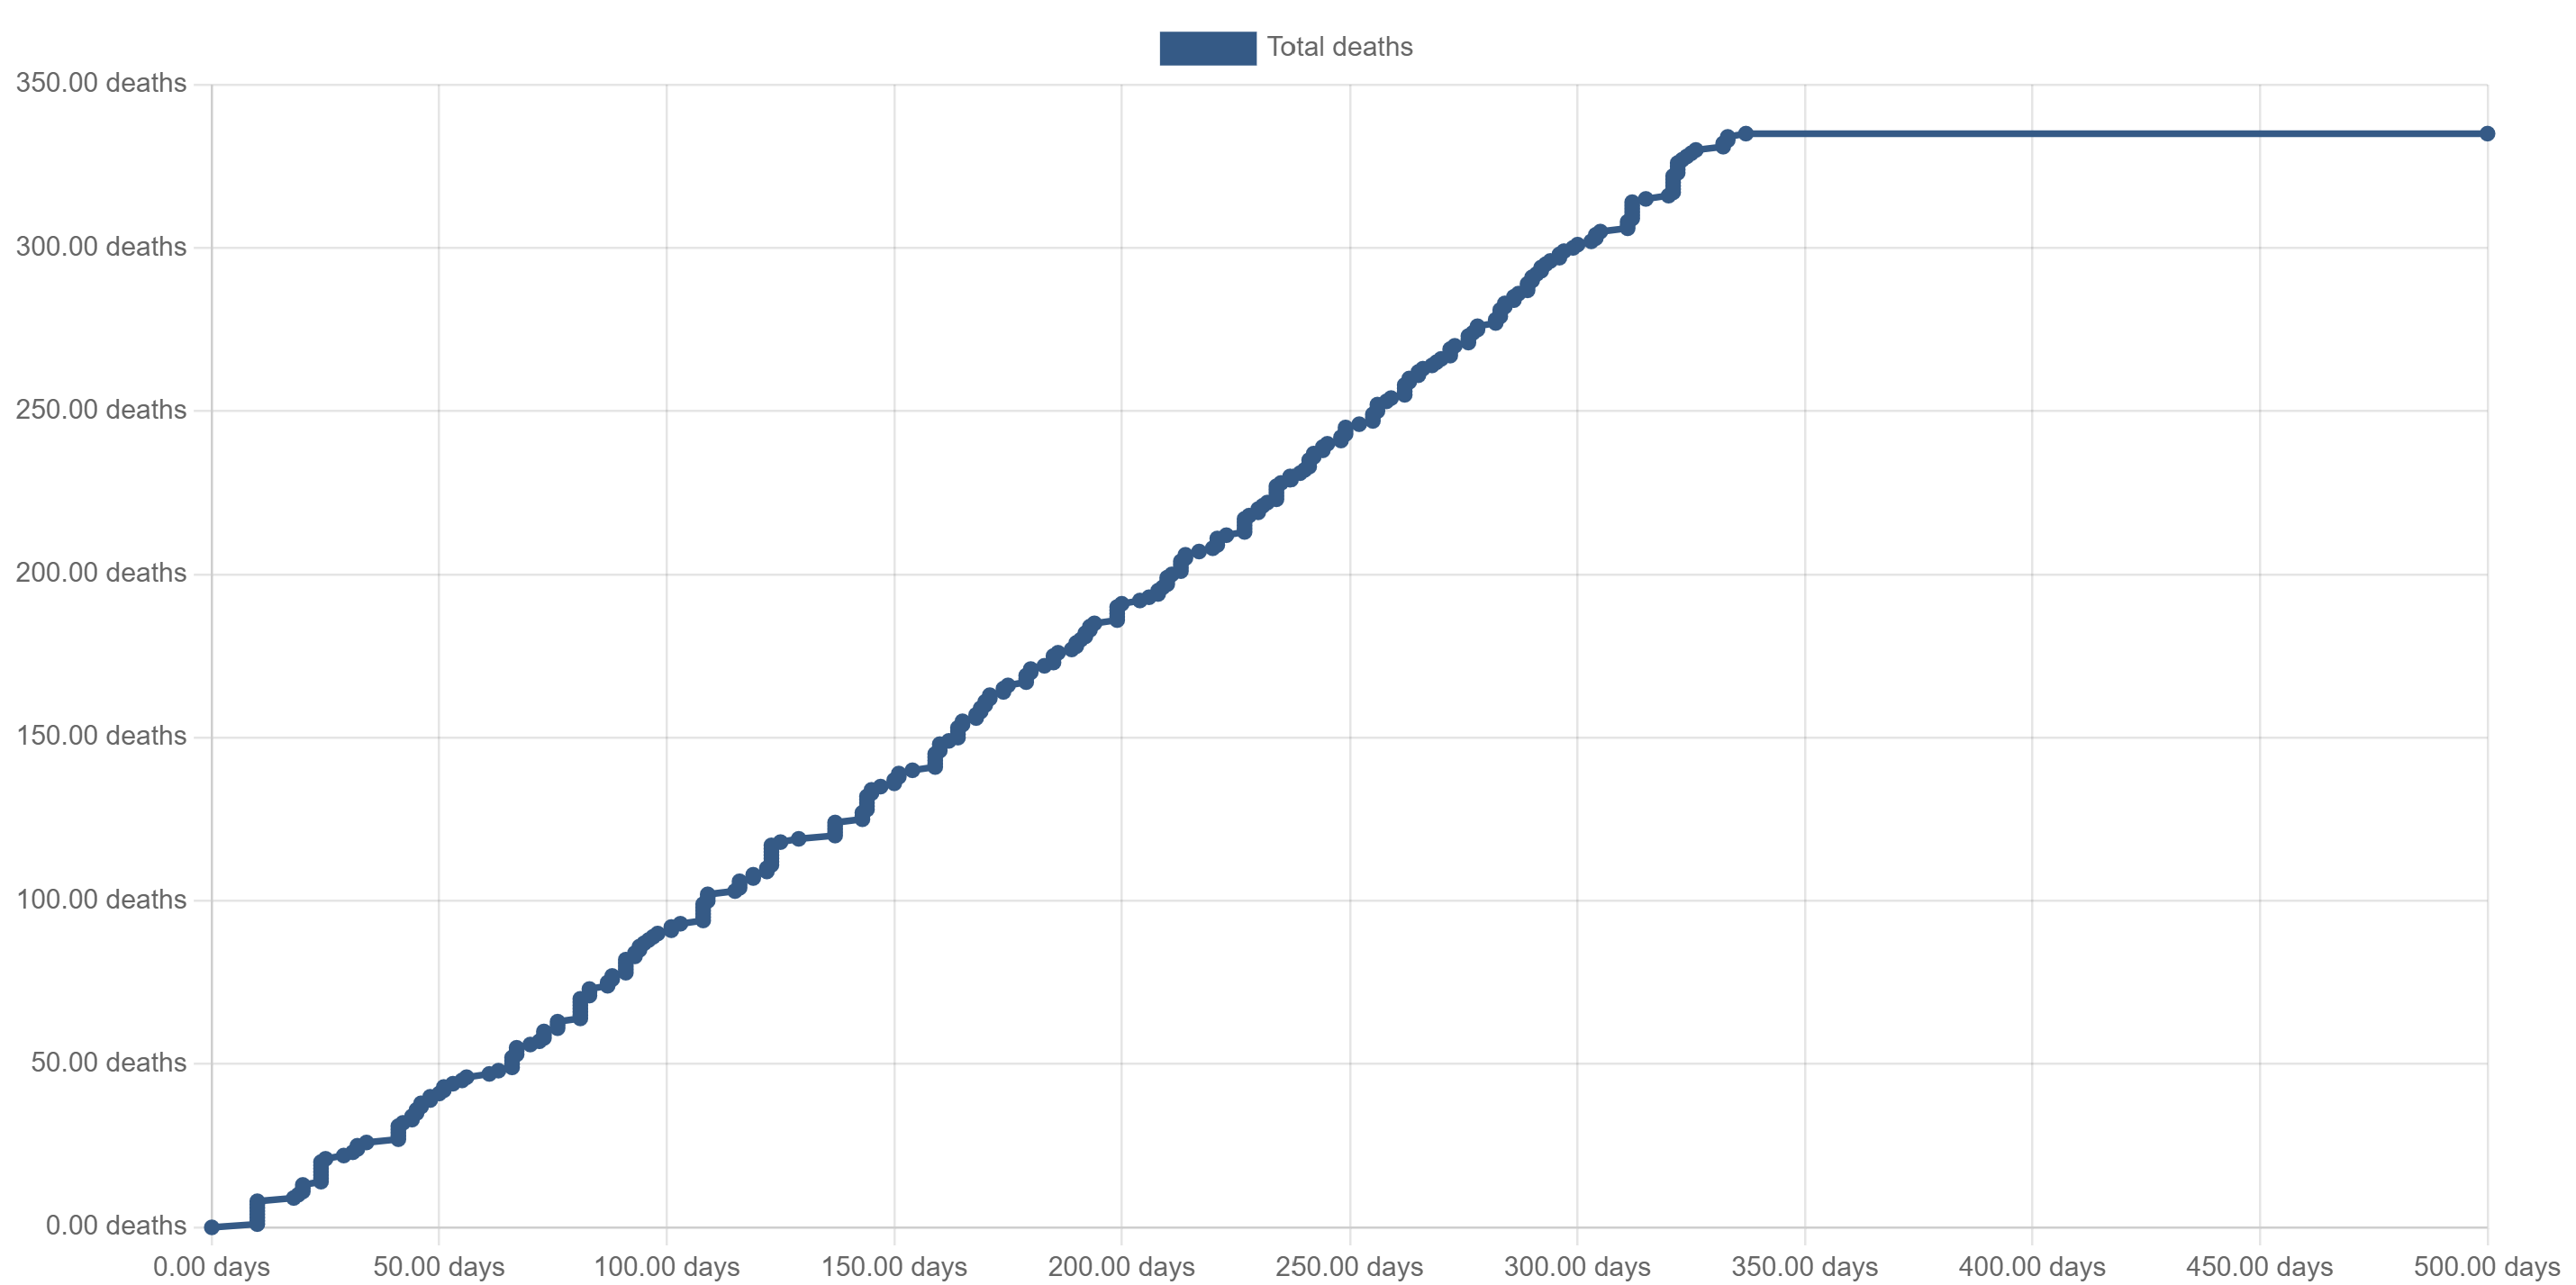
\includegraphics[width=0.8\textwidth]{007_team_5_agent_design/20-agent-2-food.png}
    \caption{Cumulative deaths per day for a 500 day simulation of 20 Team 5 agents with 2 food per agent}
    \label{fig:team5-20agents-2food}
\end{figure}

These results naturally led to the consideration of whether a homogeneous tower of Team 5 agents would achieve organisation given an infinite amount of time regardless of the number of agents provided at least two food per agent was available. We predict that this is not possible: every time an agent is replaced in the tower, its replacement is initialised with maximum selfishness and has no social network. It takes time for agents to build trust with each other but deaths occur too quickly for this happen if the settings of the tower are too strict.

\subsection*{Heterogeneous Tower Experiments}
These experiments compare the Team 5 agent with the agents designed by the other agent teams. The base parameters for all simulations are as follows:
\begin{itemize}
    \item 10 Team 5 agents, and two agents from each other team, excluding the random and selfish agents (i.e. half of the tower is Team 5).
    \item 6 food per agent
    \item 3 day reshuffle period
    \item 20 day simulation
\end{itemize}

\subsubsection*{Simulation Length}
\begin{figure}
    \centering
    \begin{minipage}{0.45\textwidth}
        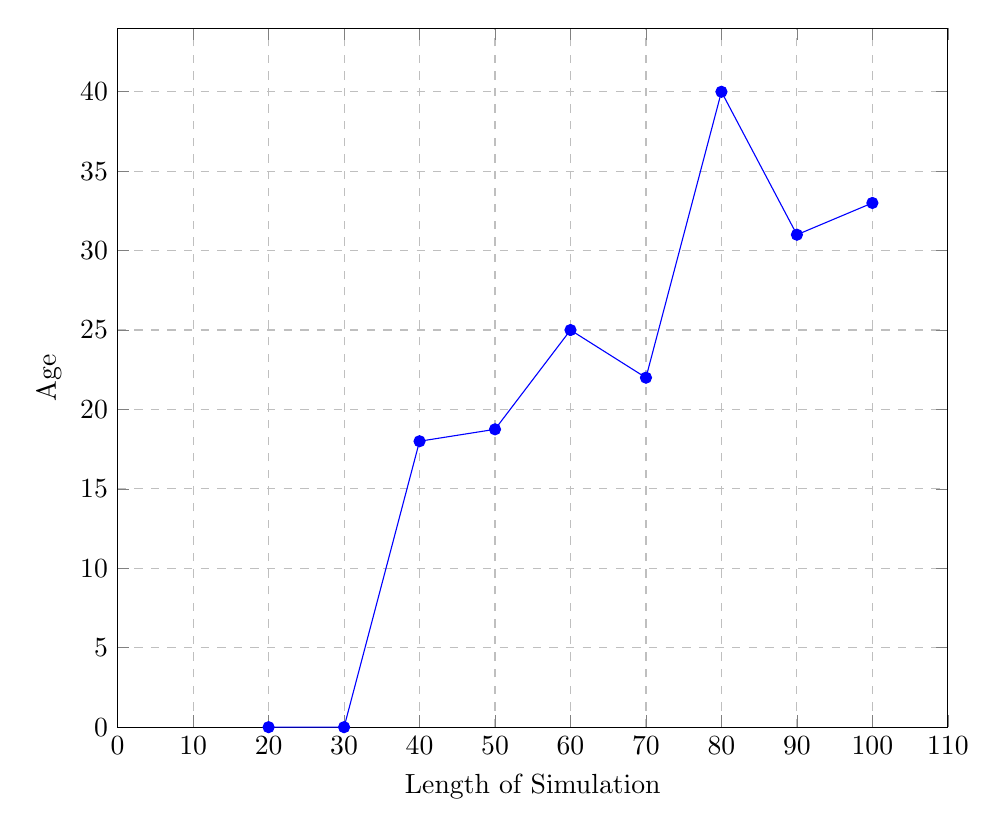
\begin{tikzpicture}
            \begin{axis}[
                width=\textwidth,
                ymin=0,
                xmin=0,
                xlabel=Length of Simulation,
                ylabel=Age,
                ymajorgrids=true,
                xmajorgrids=true,
                grid style=dashed,
            ]
            \addplot[mark=*,blue]
                coordinates{
                    (20, 0)
                    (30, 0)
                    (40, 18)
                    (50, 18.75)
                    (60, 25)
                    (70, 22)
                    (80, 40)
                    (90, 31)
                    (100, 33)
                };
            \end{axis}
            \end{tikzpicture}
            \caption{Average age upon death vs length of simulation. Points with age 0 mean no agent died during those simulations.}
            \label{fig:team5-exp-sim-length}
    \end{minipage}
    \hspace{0.05\textwidth}
    \begin{minipage}{0.45\textwidth}
        \begin{tikzpicture}
            \begin{axis}[
                width=\textwidth,
                ymin=0,
                xmin=0,
                xlabel=Food per agent,
                ylabel=Deaths,
                ymajorgrids=true,
                xmajorgrids=true,
                grid style=dashed,
            ]
            \addplot[mark=*,blue]
                coordinates{
                    (3, 7)
                    (4, 6)
                    (5, 2)
                    (6, 0)
                    (7, 1)
                };
            \end{axis}
            \end{tikzpicture}
            \caption{Number of deaths vs food per agent ratio}
            \label{fig:team5-exp-food-per-agent}
    \end{minipage}
\end{figure}
\ToDo{Check this result: is it actually true?}
Figure \ref{fig:team5-exp-sim-length} shows the relationship between the length of the simulation and the average age of Team 5 agents when they die: the graph shows a positive trend of increasing average age, implying that Team 5 agents perform better over time.

\subsubsection*{Food Per Agent}
Figure \ref{fig:team5-exp-food-per-agent} shows the effect of increasing the amount of food on the platform: the graph trends downwards as expected, showing that more food reduces the number of deaths.

\subsubsection*{Reshuffle Period}
\begin{figure}
    \centering
    \begin{minipage}{0.6\textwidth}
        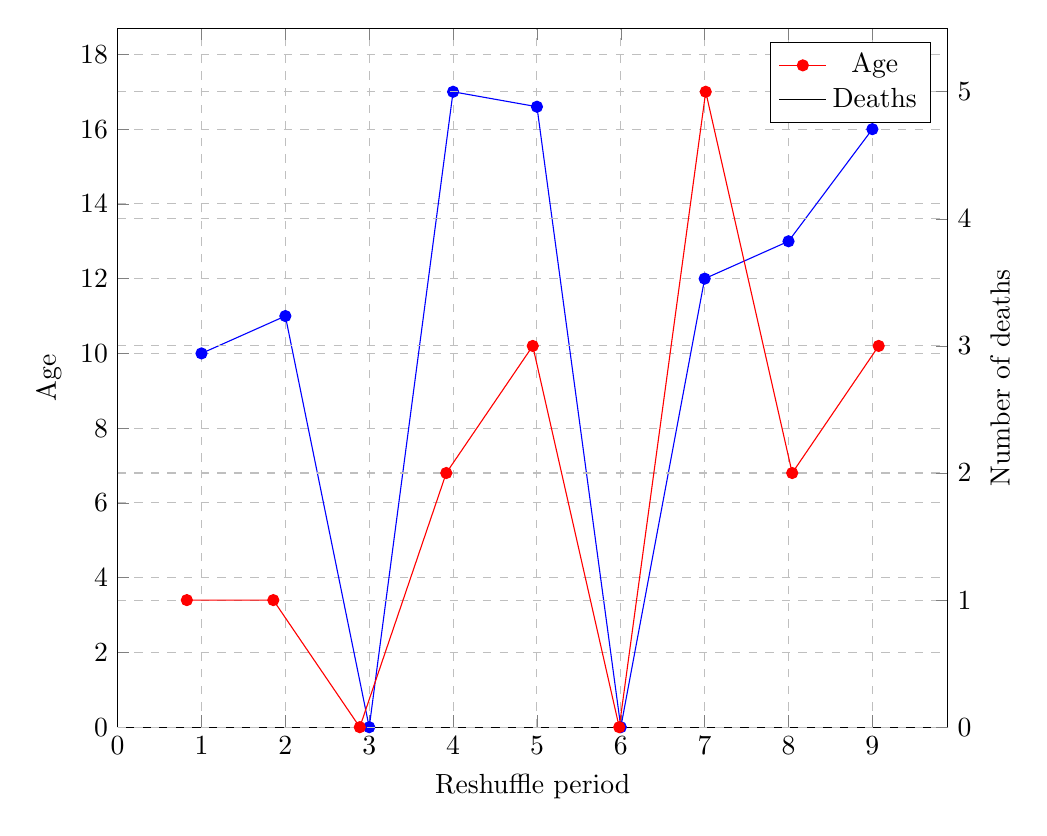
\begin{tikzpicture}
            \begin{axis}[
                width=\textwidth,
                axis y line*=left,
                ymin=0,
                xmin=0,
                xlabel=Reshuffle period,
                ylabel=Age,
                ymajorgrids=true,
                xmajorgrids=true,
                grid style=dashed,
            ]
            \addplot[mark=*,blue]
                coordinates{
                    (1, 10)
                    (2, 11)
                    (3, 0)
                    (4, 17)
                    (5, 16.6)
                    (6, 0)
                    (7, 12)
                    (8, 13)
                    (9, 16)
                }; \label{leg:team5-age}
            \addlegendentry{Age}
            \end{axis}
            
            \begin{axis}[
                width=\textwidth,
              axis y line*=right,
              axis x line=none,
              ymin=0,
              ylabel=Number of deaths,
              ymajorgrids=true,
              xmajorgrids=true,
              grid style=dashed,
            ]
            \addplot[mark=*,red]
                coordinates{
                    (1, 1)
                    (2, 1)
                    (3, 0)
                    (4, 2)
                    (5, 3)
                    (6, 0)
                    (7, 5)
                    (8, 2)
                    (9, 3)
                }; \label{leg:team5-deaths}
            \addlegendimage{/pgfplots/refstyle=leg:team5-age}\addlegendentry{Age}
            \addlegendimage{/pgfplots/refstyle=leg:team5-deaths}\addlegendentry{Deaths}
            \end{axis}
            \end{tikzpicture}
    \end{minipage}
    \caption{Average age upon death and number of deaths vs reshuffle period}
    \label{fig:team5-exp-reshuffle-period}
\end{figure}

% \subsection*{Comparing Team 5 with Other Agent Teams: Friend or Foe?}
% The next batch of experiments involved simulations with 10 Team 5 agents and 10 agents from another team to measure performance with other teams individually. Each of these experiments were run for 100 days, with the food per agent ratio varied to see how each agent type works together with varying food supply.

% We have highlighted those agents that work well with the Team 5 agent (``friends'') and those that do not (``foes''), given that one of the aims is to minimise the number of deaths in the tower. The chosen performance metrics are therefore the number of deaths and the average age upon death.

% \subsubsection*{Friends}
% Team 5 has the best survival rate when sharing the Tower with Team 4; simulations showed that with a food per agent ratio of 7 or 8, no deaths occurred within 100 days. Even when this ratio was 6 food per agent, there were only five deaths: three from Team 5 and two from Team 4, with average ages of 11.6 and 12.5 days upon death, respectively.

% Team 5 also performs well with Team 7 and Team 3; these results are shown in Tables \ref{tab:team5-team5-team7} and \ref{tab:team5-team5-team3}, respectively.

% \begin{table}
%     \centering
%     \begin{tabular}{|c|c|c|c|}
%         \hline
%         \textbf{Food per agent ratio} & \textbf{6} & \textbf{7} & \textbf{8}\\
%         \hline
%         Team 5 deaths and average age upon death       & 4, 46 & 0, 0 & 0, 0\\
%         \hline
%         Team 7 deaths and average age upon death       & 4, 19.5 & 3, 25 & 1, 22\\
%         \hline
%     \end{tabular}
%     \caption{Results of a Tower consisting of Team 5 and Team 7 agents}
%     \label{tab:team5-team5-team7}
% \end{table}

% \begin{table}
%     \centering
%     \begin{tabular}{|c|c|c|c|}
%         \hline
%         \textbf{Food per agent ratio} & \textbf{6} & \textbf{7} & \textbf{8}\\
%         \hline
%         Team 5 deaths and average age upon death       & 11, 41 & 7, 63 & 1, 15\\
%         \hline
%         Team 3 deaths and average age upon death       & 8, 45 & 0, 0 & 0, 0 \\
%         \hline
%     \end{tabular}
%     \caption{Results of a Tower consisting of Team 5 and Team 3 agents}
%     \label{tab:team5-team5-team3}
% \end{table}

% \subsubsection*{Foes}
% Team 5 does not perform well with either Team 6 or Team 2. When paired with Team 6, the Team 6 agents die often and have less than half the lifespan of the Team 5 agents. This issue persists with increased amount of food on the platform.

% When paired with Team 2, the Team 2 agent has significantly fewer deaths than the Team 5 agent and also has a longer lifespan. These results suggest that this agent pairing is unable to self-organise, with the potentially more selfless Team 5 agents left to starve by the Team 2 agents. This is because the Team 2 agents do not communicate except to ask for the HP of other agents.

% The Team 5 agent is least compatible with random agents (i.e. agents which take a random amount of food). The total number of deaths is highest and average age upon death is lowest with this pairing. The life expectancy also does not improve with more food on the platform.

\subsection*{Self-Organisation With Other Agents}
The overall aim within the tower is for agents to self-organise and create a stable society. Tests were run to investigate how compatible the Team 5 agent is with each of the agents designed by each of the other teams. Simulations were run with a tower consisting of Team 5 agents and one other agent type, with seven agents each and five food available per agent, to see whether they could self-organise within 100 days. These results are shown in Table \ref{tab:team5-self-org-agents}

\begin{table}
    \centering
    \begin{tabular}{|c|c|c|c|c|c|}
        \hline
        \textbf{Agent type} & \textbf{Team 2} & \textbf{Team 3}& \textbf{Team 4} & \textbf{Team 6} & \textbf{Team 7}\\
        \hline
        Team 5 deaths & 25 & 5 & 0 & 25 & 12 \\
        \hline
        Other agent deaths & 19 & 5 & 0 & 35 & 8 \\
        \hline
        Organisation? & NO & 67 days & 0 days & NO & 62 days \\
        \hline
    \end{tabular}
    \caption{Team 5 interactions with other agents}
    \label{tab:team5-self-org-agents}
\end{table}

\section{Conclusion}\label{sec:team5-conclusion}
The Team 5 agent is capable of achieving self-organisation within the tower provided the simulation parmaeters are not too strict. A large number of agents within the tower greatly inhibits the agent's ability to self-organise, but they are capable of organising when there is the food per agent ratio is at least 2, for low agent numbers. This demonstrates the reliance on communication and sharing of knowledge in order to solve the problem of long-term survival in the tower.

During the presentation for this coursework, Professor Pitt compared the Team 5 agent's strategy to theory from Ober, who stated that ``alignment is an epistemic process, predicated on the right people having and using the right information in the right context'' \cite{ober_athens}. We had not considered this theory when designing our agent, however in a sort-of convergent evolution we observed this in the randomeness and large variation in the Team 5 agent's ability to self-organise, and the events that need to take place for this to be successful.

\chapter{Team 6 Agent Design}\label{team_6_agent_design}
\chapter{Team 7 Agent Design}\label{team_7_agent_design}

\section{Overview}
\label{sec: Team 7 Overview}
This chapter outlines the design and findings of Team 7's agent. The primary goal of team 7 was to emulate human behaviour closely and to replicate the normal variation in personality types exhibited in a typical human population. This would then enable analysis into whether particular personality types exhibited particular behavioural patterns or are more conducive to self organisation and thus acheiving the goal of sustainability in a collective action problem.

\section{Agent Design}
\label{sec: Agent Design}
There are 3 key elements that define the agent: its personality, behaviour and memory. The personality defines a given agent at its core, and for the purpose of this experiment is kept constant throughout a given simulation. An agents behaviour is influenced by its personality, memory (a record of its experiences) and the environment. The environment can include current floor, food available and interaction wit other agents. The personality and behaviour then combine to influence the various decisions that the agent makes over the course of the simulation. 
This basic agent framework is illustrated in \Cref{agent_flow}.

\begin{figure}[H]
    \begin{center}
        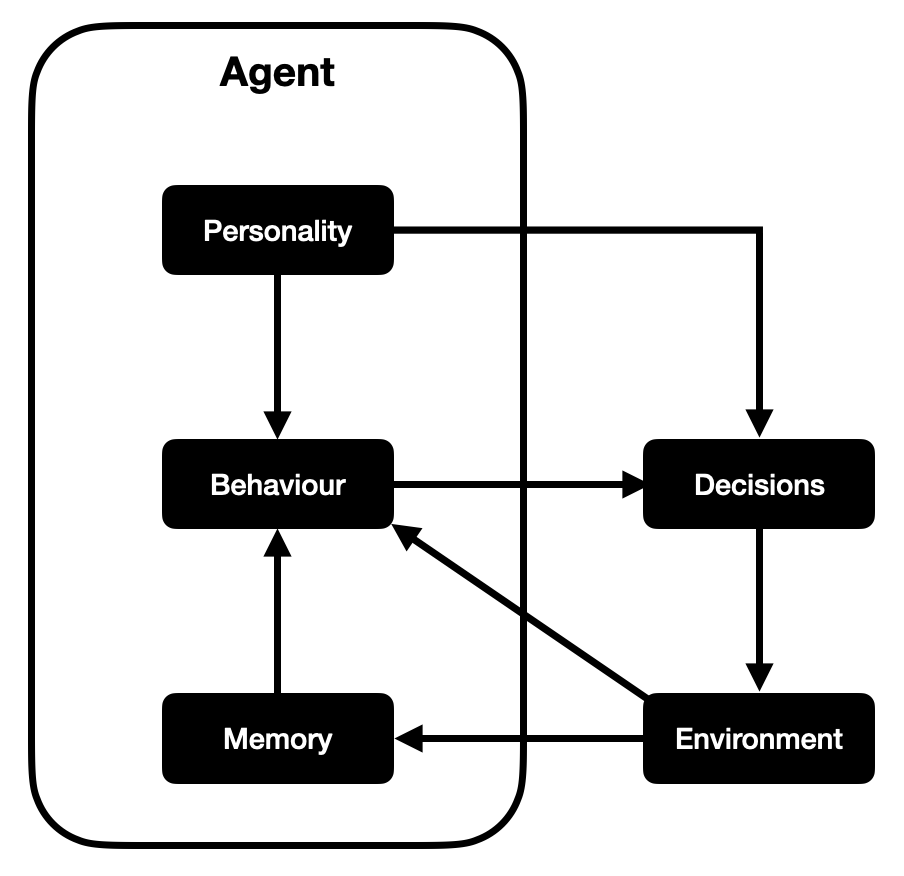
\includegraphics[width=6cm]
        {009_team_7_agent_design/Images/agent_flow.png}
    \end{center}
    \caption{Agent framework.}
    \label{agent_flow}
\end{figure}

\subsection{Personality Traits}
\label{subsec: Agent Design}
The use of personality traits to attribute human characteristics to our agents is a construct derived from Robert R. McCrae and Paul Costa's 5 factor theory of personality. McCrae and colleagues discovered that the big five traits are surprisingly universal which was confirmed by a study that looked at people from more than 50 different cultures. They determined that the five personality traits could be used to accurately model the human psychological framework.

The five personality dimensions consist of: 
\begin{itemize}
    \item  \textbf{Openness}: The degree to which an individual is willing and eager to have new experiences. This also has implications for creativity and problem solving. An individual with low openness will behave more traditionally and will be less welcoming to change. For an agent in the tower this means a high openness score means that they are less impacted by floor changes and thus its behavioural characteristics are not varied as much. Conversely a low openness score means an agent is significantly impacted by change such as arriving at a lower floor which increases their greediness more than it would an agent with a higher openness score. Openness also influences responsiveness which dictates how much an agent is willing to accept or requests or treaties.
    \item  \textbf{Conscientiousness}: The degree of conscientiousness of an individual determines their level of organization, discipline and thoughtfulness. Conscientious individuals are also more strategic and forward thinking. In the context of this experiment, a high conscientiousness score means an agent will demonstrate greater learning from its experiences, as it will identify underlying trends in these experiences in order to make strategically better decisions. A more planning-oriented agent of such will also give greater importance to collaborating with other agents.
    \item  \textbf{Extraversion}: The extent to which an individual is willing and eager to socialise and interact with other individuals. An extroverted individual is more likely to occupy positions of leadership and influence. The extraversion score affects the responsiveness. A high extraversion score increases the likelihood of positive social interaction such as accepting requests or treaties. 
    \item  \textbf{Agreeableness}: An individual with high agreeableness will exhibit greater degrees of kindness, trust and altruism. Whereas an individual with low agreeableness will demonstrate a lack of sympathy and may be spiteful or manipulative of others. Therefore, greediness and kindness are initialised by agreeableness and scaled accordingly. Agreeableness also has influence over responsivenes in the same way that openness and extraversion do.
    \item  \textbf{Neuroticism}: The neuroticism trait dictates the emotional stability of an individual. It is associated with greater proneness to anxiety, irritability and mood swings. In the extreme case, individuals can experience regular fluctuations in their character. Therefore, an agent that is high in Neuroticism will commit actions that may seem unreasonable or illogical. The way this is implemented is that neuroticism will create random day-to-day volatality in the greediness and kindness levels of an agent. Since greediness and kindness directly control the amount of food taken, an agent with higher Neuroticism may either intend to take an inadequate or excess amount of food.
\end{itemize}

Any time a new agent is deployed it is initialised with a value for these traits ranging from 20-80. We did this in order to exclude extreme personality traits on either end. The personality traits assigned to an agent are innate and unchanged for the duration of the simulation. This is done in order to emulate how traits remains fairly constant over a person's life.

\subsection{Behavioural Traits}
\label{subsec: Behaviour}
In contrast to personality traits, behavioural characteristics of an agent change over the course of the simulation. The behaviours are initialized based on the agent's personality traits and can range from 0-100 over the lifetime of the agent. These behaviours are then updated daily by environmental factors such as food availability, floor changes and interactions with other agents. 

The behaviour characteristics are described below:
\begin{itemize}
    \item  \textbf{Greediness}: This is the degree to which an agent behaves selfishly, specifically with regards to the amount of food it takes. The greediness value is initialised by the agent's agreeableness score meaning that high agreeableness will result in low initial greediness and vice versa. The greediness value is subsequently adjusted throughout the simulation run by the following factors: 
    
    \begin{itemize}
        \item Being in a critical health state increases greediness.
        \item Eating no food increases greediness by a quadratic factor with respect to the number of days since the last food intake.
        \item Agents display increased levels of greediness in response to being placed at a lower floor during the reshuffle and vice versa. The degree to which this changes is dependent on the openness of said agent.  
        \item Based on past experience, if the agent expects food shortages on a new floor, there will be an additional boost to greediness. This adjustment has a greater impact if the agent has high level of conscientiousness.
        \item Neuroticism can cause sporadic daily fluctuations in the greediness of an agent. A higher neuroticism results in more substantial daily changes of the relevant behaviours.
    \end{itemize}
    
    \item  \textbf{Kindness}: An agent with a high kindness value will demonstrate greater sympathy for other agents and will be more supportive of the wider social cause. Kinder agents will take less food and will be more likely to collaborate with other agents. 
    
    Similar to greediness, kindness is initialised by the agent's agreeableness score meaning that high agreeableness will result in high initial kindness. The kindness value is subsequently adjusted throughout the simulation run by the following factors:
    
    \begin{itemize}
        \item Agents display increased levels of kindness in response to being placed at a higher floor during the reshuffle and vice versa. The degree to which this changes is dependent on the openness of said agent. A lower the openness the greater the change.
        \item Neuroticism can also result in sporadic daily fluctuations in the kindness of an agent. A higher neuroticism results in more substantial daily changes of the relevant behaviours. 
    \end{itemize}
    
    \item  \textbf{Responsiveness}: 
    
    This behaviour influences the likelihood of an agent accepting the treaties of other agents. It is initialized as the average of openness, extraversion, and agreeableness. 
    
    In the current implementation the responsiveness trait does not vary during the simulation. In an implementation where dishonesty is factored in, the agent would keep record of the trustworthiness of each agent that it interacts with. If other agents are largely untrustworthy, overall responsiveness would go down proportionally. 
    
\end{itemize}

\subsection{Operational Memory}
\label{subsec: Operational Memory}
The memory structure of the agent behaves analogously to human memory. It serves to store experiences and data acquired across the lifespan of the agent. These experiences and data serve to influence the agent's behaviour, inform it's decisions, and enhance its survival and organisation capabilities. 
Below is a description of all the elements of information stored in the agent's memory:

\begin{itemize}
    \item  \textbf{orderPrevFloors}: A chronologically ordered list of the floors that the agent has been in. 
    \item  \textbf{prevFloors}: A map of all the floors that the agent has experienced. This keeps track of the number of days spent on each given floor and the average food that was available whilst the agent was on that floor.
    \item  \textbf{currentDayonFloor}:The number of days the agent has spent on the current floor.
    \item  \textbf{currentFloorRisk}: This is the level of risk to the survival of the agent associated with the current floor. 

    \item  \textbf{daysHungry}: The number of consecutive days the agent has not consumed food.
    \item  \textbf{seenPlatform}: This variable is used to remember if the agent has seen the platform. The agent uses this to decide when to prepare for a new day.
    \item  \textbf{prevAge}: The age of the agent on the previous day.
    \item  \textbf{prevHP}: A record of the HP at the end of the previous day.
    \item  \textbf{foodEaten}: The amount of food consumed the previous day.
    \item  \textbf{receivedReq}: This is a variable that indicates whether the agent has decided to abide by a request made in a message. A false value indicates that no requests have been accepted. 
    \item  \textbf{takeFood}: This stores the amount of food an agent has requested to be taken. It is initialised with a value of -1 if there are no accepted requests.
    \item  \textbf{leaveFood}: This stores the amount of food an agent has requested to be left. It is also initialised with a value of -1 if there are no accepted requests.
\end{itemize}

\subsection{Floor Risk Estimation}
\label{subsec: Floor Map}
Upon a floor reshuffle, the agent uses its experiences from past floors in order to build an expectation of the level of risk it associates with the new floor that it has been assigned to. The first step to doing this is to generate a prediction for the amount of food that will be available on the current floor. 

In order to make this estimate, the agent utilises the prevFloors map from its memory. This contains information on the average food that was available on each floor that the agent has already been on. The agent approximates the relationship between the floor level and the average food available on that floor. For example, let us take an agent that has been on floors 10 and 6, and is now assigned to floor 8. The agent will calculate the linear function which corresponds to the average food on floors 6 to 10. It will then use this function to obtain the estimate for the food it expects on floor 8. 

The above assumes that the agent has experienced floors both above and below the current floor. In the scenario where the agent has only experienced floors either below or above its current floor, the agent will extrapolate the trend line for the average food from the closest experienced floor. 

Next, the agent determines the level of risk to its survival that it associates with the current floor. It does this by checking whether the estimated amount of food would be enough to exit a hypothetical critical state and enter the weak state. The difference between the required food and the estimated food will determine the floor risk value. The floor risk value will subsequently adjust the agent's greediness. 

Note that since higher levels of strategising are associated more with conscientiousness agents, it makes sense for their estimates to be more pessimistic. Therefore, they will under-estimate food availability and the floor risk will have a greater impact on their greediness. In the case of less conscientiousness agents, who would be both less planning-oriented and also more optimistic, the food estimation is higher and the risk estimator is weighed down.

\section{Agent Operation}
\label{sec: Agent Operation}
This section outlines the particulars of agent operation and decision making.

\subsection{Main Operation}
\label{subsec: Main Operation}
At the point where each agent is deployed into a simulation, its personality traits, behavioural characteristics and memory bank are initialised. 

Once initialisation is complete, the agents check their inbox for messages, requests or treaties. This is done every tick to ensure messages are detected from the floors above and below. When a message, request or treaty is found in the inbox, a function calls the corresponding handler to the message type. The handlers then decide whether a request or treaty is accepted and the relevant actions performed. This is further discussed in later sections. 

Once the inbox is handled, the agent checks whether a floor change has occurred and updates the floor Map (prevFloors) with the current available food on the platform for the day. The agent also completes a Floor risk assessment which has been outlined in the previous two sections. 

The flow chart in \Cref{fig: operation flow chart} outlines the decisions made concerning how much food to take.

\begin{figure}[h!]
    \begin{center}
        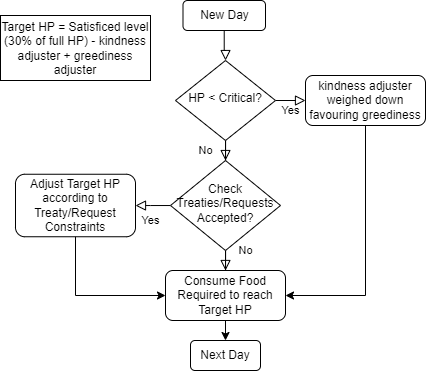
\includegraphics[scale=0.75]{009_team_7_agent_design/Images/v2.drawio.png}
    \end{center}
    \caption{Food taking decision flow chart.}
    \label{fig: operation flow chart}
\end{figure}

Upon completion of the memory bank updates and risk assessment routines, the agent then enters its food consumption routine. This routine runs only once per day when the platform is on the agent's floor. The routine begins by assessing whether the agent's health has been critical for multiple days, if this is the case the agent overrides any requests in effect and prioritises getting its health out of critical (Note however no treaties that prevent the agent from leaving critical HP would be accepted by the agent and thus no treaties would be broken at this point, treaty conditions are detailed in a later section). The kindness adjuster is weighted down and the TakeFood function is executed. If the agent's health is not critical the routine evaluates whether it can abide within the constraints imposed for accepted treaties and requests. Once the constraints are in place the TakeFood function is executed in accordance to the greed and kindness adjusters within the bounds of the request/treaty constraints. 

Once the routine is complete the seenPlatform variable is reset to indicate the end of the day.

\subsection{Messages}
\label{subsec: Messages}
Although not a crucial feature of the final agent strategy - reasonable consideration went into deciding how to leverage messaging to better serve an agent during a simulation of the tower.

In order to think about how messaging could benefit the agent, two scenario's can be considered - one where the agent is sending messages to make an alert, enquiry or request and the converse, where an agent receives messages and can perform some action based on the incoming information or request.
\subsubsection{Sending Messages}
\label{subsubsec: Sending Messages}
The agent's behaviour is majorly determined by the intrinsic characteristics that constitute the agent's personality and so it was deemed that sending messages to gather information served no significant additional purpose as the new information would not have any influence on the next decision made. It is, however, important to benefit the collective effort of maintaining survival as a population - therefore an agent will send a reply to acknowledge information from other agent's and respond to requests stating whether they can comply.

\subsubsection{Receiving Messages}
\label{subsubsec: Receiving Messages}
The agent may adapt its behaviour upon receipt of request messages from other agent's. The criteria that must be met in order to comply with a request is as follows; 

\begin{itemize}
  \item The agent's extraversion rating must be higher than 5
  \item The agent's kindness rating must be higher than it's greediness rating
  \item The agent must not have been at critical health for \(\ge\) (the max \# of days at critical - 3)
\end{itemize}

If all of this criteria is met the agent will comply with the request, and it will reject the request if any of the conditions above are not met.

In all cases a truthful reply is sent from the agent to the message sender in an attempt to benefit the collective.

\subsection{Treaties}
\label{subsec: Treaties}
Treaties are the mechanism by which agents can communicate their needs to each other and organise themselves in way that is mutually beneficial.  

\subsubsection{Rejecting Proposed Treaties}
\label{subsec: Rejecting Treaties}
Treaties are rejected on the basis of certain criteria, these `conditions' reflect proposed treaties that are detrimental to the health of Team 7's agents at the expense of other agents. The following are the main criteria for rejecting treaties:

\begin{enumerate}
    \item 
    \textbf{Personality and behaviour traits:} \newline
    Treaties that are proposed to agents that have a less than average responsiveness are automatically rejected as this aligns with our aim to replicate human responses with agents. Note that responsiveness is an average of agreeableness, openness and extroversion. Thus most personality traits are taken into account. Similarly, an agent with conscientiousness less than 33\%\ lacks the intuition to plan for future events and thus is casual in its approach to treaties, resulting in viable treaties being rejected. This shows our commitment to having agents mirror their personality traits in the actions that they take.
    
    \item 
    \textbf{Unfavourable Condition Operators for Condition Types HP \&\ Available Food:} \newline
    If the condition type of a particular treaty is \textbf{HP} OR \textbf{Available Food} AND the the condition operator is \textbf{LE} OR \textbf{LT}, then the treaty is unfeasible for survival as an individual and/or collective. It is also unreasonable to assume realistic agents that mimic human behaviour would accept any alliances in which they were bound to a limited amount or percentage of food when their health is at the critical level. Thus all treaties that have the ability to put our agents in this position are rejected.
    
    \item 
    \textbf{Unfavourable Condition Operators for Condition Type Floor:} \newline
    If the condition type is \textbf{Floor} AND the the condition operator is \textbf{GE} OR \textbf{GT}, then the treaty is rejected. This is again due to the overwhelming risk agents are exposed to when they are on a floor with a scarcity of food and resources - they will likely be critical and thus shouldn't be bound by treaties that limit their food intake.
    
    \item 
    \textbf{Detrimental Request Operators:}\newline
    Any treaty, that uses the \textbf{LE} OR \textbf{LT} request operators will be rejected. This is due to the fact that the request types are concerned with leaving a certain amount or percentage of food and thus if being asked to limit the lower bound of our food intake, our agent may consume a larger than necessary amount/percentage of food and result in other agents starving to death. This ultimately defeats the purpose of self-organisation.
    
    \item 
    \textbf{Treaties active at the Critical Level:} \newline
    If the condition type holding up a certain treaty is \textbf{HP} and the condition value is less than the value required for the agent to be at the weak level, then such a treaty is not accepted. This is purely because of the risk it poses to our agent when we are below the weak level and require food but are bounded by a signed treaty that doesn't allow us to take any.
    
    \item 
    \textbf{Unreasonably long Duration of Treaties:} \newline
    The duration of the treaty is also an important consideration to take into account. For a treaty to be fully effective, it must persist for an adequate amount of time such that it is used beneficially for self-organisation. Therefore treaties in which our agents' actions are restricted for a long duration are rejected to avoid the negative impact these outdated treaties could have. 
    
    \item 
    \textbf{Clash of treaties:} \newline
    Each new treaty is compared to the existing active treaties that are already stored in the agent's memory. If a treaty is incompatible with those that are already active, then the agent will reject such treaties. For example: treaties that are based on the same request type cannot ask for conflicting amounts of food, for e.g. If a treaty asking us to leave exactly 10 units of food has been accepted, then a freshly proposed treaty requesting to leave less than 7 units of food has to be rejected to avoid conflict.
\end{enumerate}

Once a treaty is rejected, a confirmation of the rejection is sent to the proposer of the treaty and a message noting the outcome of the treaty is added to the log file at the output.

\subsubsection{Accepting Treaties}
\label{subsec: Accepting Treaties}

Treaties are accepted if the aforementioned rejection criteria are not satisfied and the agent has the relevant personality traits and behaviour. In particular, the responsiveness behaviour characteristic of a given agent should be greater than 50 and the personality trait conscientiousness should be greater than 33. 
\newline

All accepted treaties are stored in the active treaties field of the Base Agent thus allowing for the conflict criteria to be checked by iterating through the \texttt{activetreaties} map. Theoretically all treaties that get through the vetting process are either beneficial to the agent or the wider group and do not make the agent prone to an earlier than expected death as a result of accepting said treaty.

\subsubsection{Treaty Usage}
\label{subsec: Treaty Usage}
All treaties accepted are stored in the active treaties field of the base agent. Since treaties that could negatively impact the agent are rejected, ones that are signed can be followed, without further checking. 

Before an agent takes its share of food, The condition statements pertaining to active treaties are extensively checked to make sure that a Treaty is being considered only when its respective conditions are upheld. Subsequently, the agent must check the request type, value and operator. If the request type is \textit{LeavePercentFood}, it is converted to an \textit{amount} for easy comparison. 
The amount of food being taken is checked for compatibility with the amount of food that is to be left. If this is not the case then the \textit{foodtotake} variable for the agent is updated accordingly.
This will repeatedly happen until the expiration date of the treaty.

\subsubsection{Treaty Formulation}
\label{subsec: Treaty Formulation}
Treaty Formulation can play an important role in creating favourable conditions, not only for the survival of the proposing agent, but also for other agents. There are three types of scenarios which trigger the agent to propose a new treaty to its surrounding agents:

\begin{enumerate}
    \item \textbf{Health:} When an agent is in critical health state it is compelled to ask the neighbour above to leave an amount of food that can allow him to survive, i.e. go from critical to weak state. This health condition for this treaty is set such that the agents who sign the treaty are not put in danger, and this also makes it more likely for the treaty to be accepted.
    
    \item \textbf{Floor:} If the conscientiousness of the agent is a above a certain threshold, meaning that the agent is relatively forward thinking and aware of their surroundings, then the agent will try to initiate a treaty with the neighbouring agent above him. This is triggered upon a floor change when the current floor is at a lower level than the previous floor. A conscientiousness agent will know that it is likely that food will be more scarce at this level and so he initiates a treaty to make survival at this floor easier.

    \item \textbf{Propagation:} A treaty that has been accepted from an agent will be propagated onward in the same direction. If the treaty is coming from downwards and the request type is `LeaveAmountFood', then the request value is increased before propagating the same treaty upwards. This must be done to ensure that the agent above leaves enough food for our agent \textit{and} the agents below us. If the agent above uses the same strategy, then this can form an efficient means of survival for all agents in the tower.
\end{enumerate}

\section{Simulations and Analysis}
\subsubsection{Significance of Treaties}
\label{sec: Simulations and Analysis}
\Cref{fig: Cumulative Deaths without Treaties} and \Cref{fig: Cumulative Deaths with Treaties} illustrate the results from simulations with treaties disabled and enabled respectively. All other factors are left as default.

\begin{figure}[h!]
    \begin{center}
        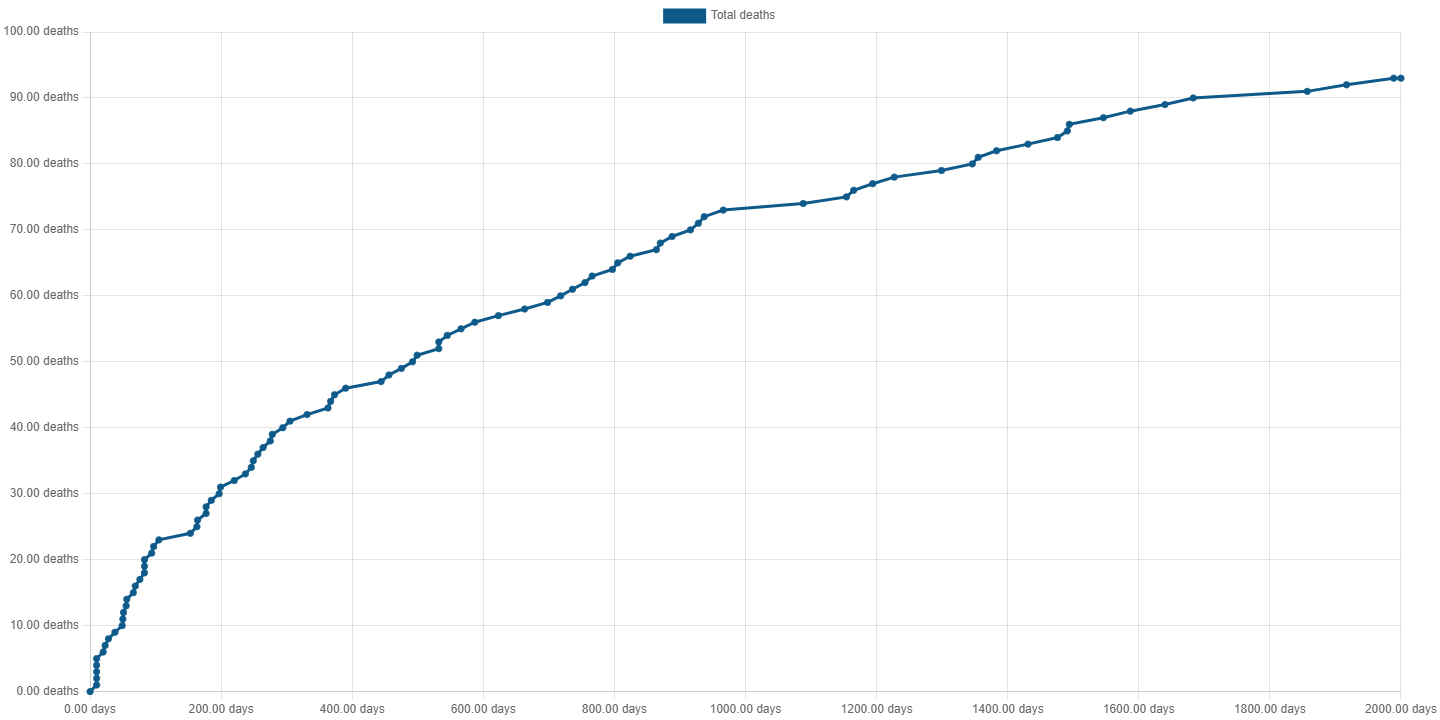
\includegraphics[scale=0.25]{009_team_7_agent_design/Images/Cumulative Deaths, WO Treaties, T7Only, 2000days, 20food, 93deaths.png}
    \end{center}
    \caption{Cumulative deaths without treaties (93 deaths).}
    \label{fig: Cumulative Deaths without Treaties}
\end{figure}

\begin{figure}[h!]
    \begin{center}
        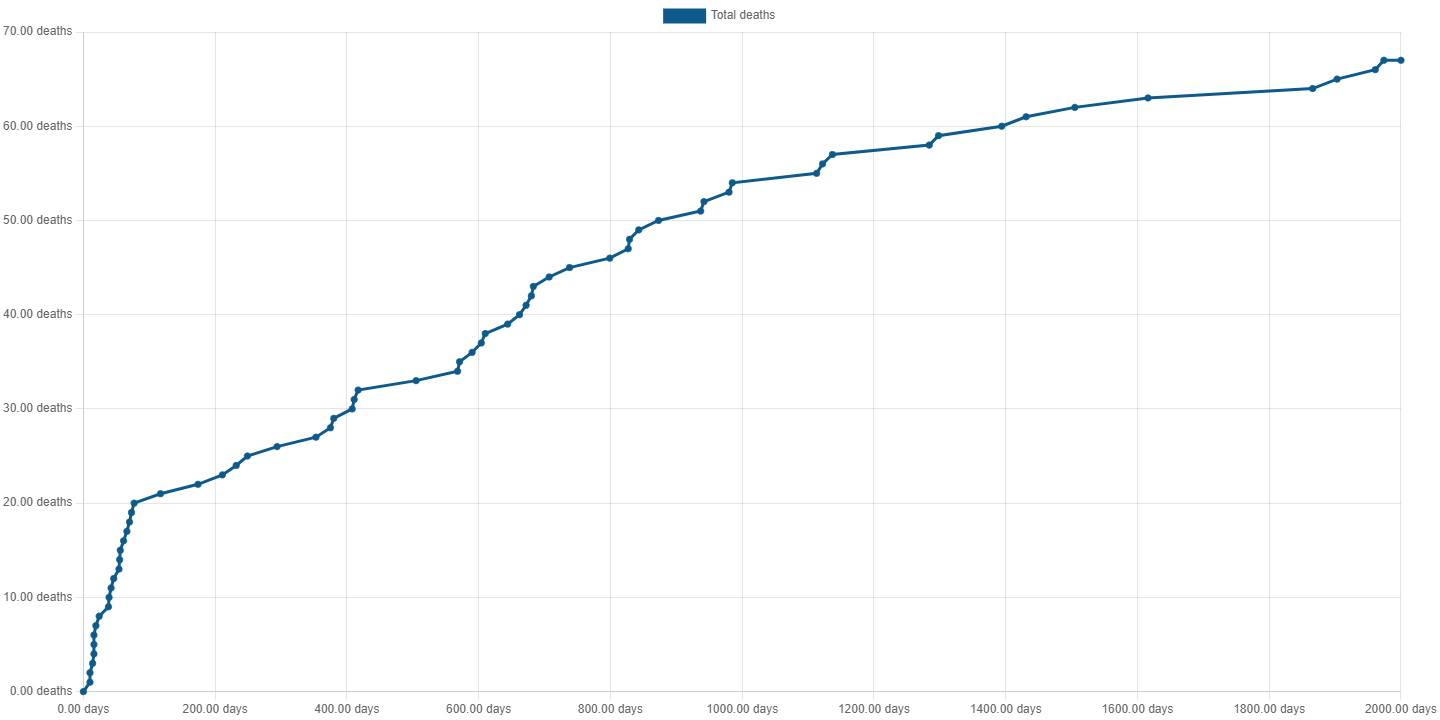
\includegraphics[scale=0.25]{009_team_7_agent_design/Images/Cumulative Deaths, With Treaties, T7Only, 2000days, 20food, 67deaths.png}
    \end{center}
    \caption{Cumulative deaths with treaties (67 deaths).}
    \label{fig: Cumulative Deaths with Treaties}
\end{figure}

This demonstrates that the agents perform better collectively when treaties are activated. This is expected as treaties enable agents to cooperate and organize the distribution of scarce food. 

\newpage
\subsubsection{Impact of Personalities}
\label{subsubsec: Impact of Personalities}

\subsubsection{Openness}
\label{subsubsec: Openness}

\Cref{fig: High Openness} and \Cref{fig: Low Openness} detail how our agents adapt to situations/scenarios differently based on varying levels of openness. In \Cref{fig: High Openness}, all the agents are spawned with openness values greater than 70 and in \Cref{fig: Low Openness}, the agents are spawned with openness values less than 30. All other personality traits are distributed as in the default case.

\begin{figure}[H]
    \begin{center}
        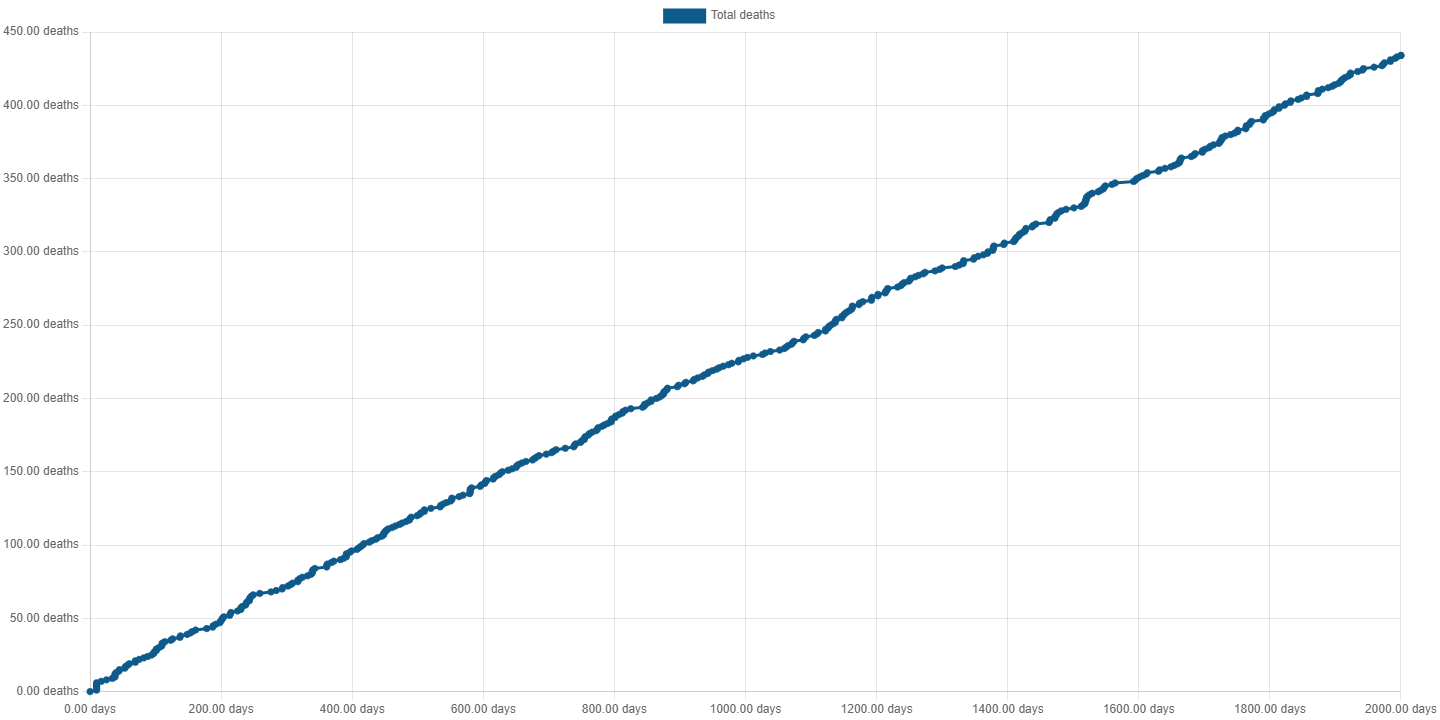
\includegraphics[scale=0.25]{009_team_7_agent_design/Images/Cumulative Deaths, With Treaties, T7Only, 2000days, 20food, High Openness, 434deaths.png}
    \end{center}
    \caption{Cumulative deaths with high openness (434 deaths).}
    \label{fig: High Openness}
\end{figure}

\begin{figure}[H]
    \begin{center}
        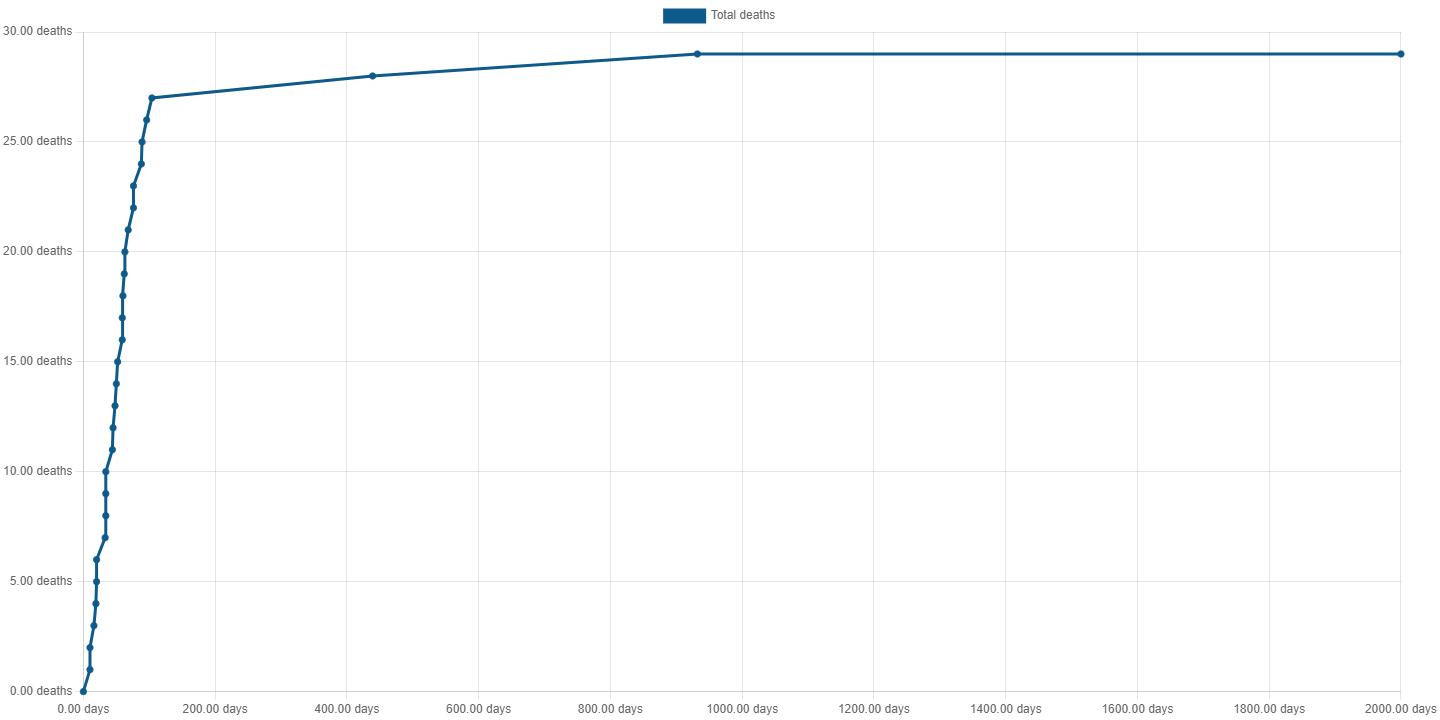
\includegraphics[scale=0.25]{009_team_7_agent_design/Images/Cumulative Deaths, With Treaties, T7Only, 2000days, 20food, Low Openness, 29deaths.png}
    \end{center}
    \caption{Cumulative deaths with low openness (29 deaths).}
    \label{fig: Low Openness}
\end{figure}

It can be observed that the agents collectively perform significantly better when openness is low, as a stabilising of the cumulative deaths curve can be seen for the agent with low openness. This can be explained by the fact that an agent with high openness will have a lower standard for accepting message requests and treaties - meaning they are more likely to agree to a request that is detrimental to their survival. Furthermore, an agent with a low openness value will be less welcoming to a change in floor and will therefore behave more cautiously. This will also improve the agents chances of survival. 

\subsubsection{Neuroticism}
\label{subsubsec: Neuroticism}

\Cref{fig: High Neuroticism} and \Cref{fig: Low Neuroticism} illustrate the results from simulations with agents with high neuroticism ($>$70) and low neuroticism ($<$30) respectively. All other traits are left as default.

\begin{figure}[H]
    \begin{center}
        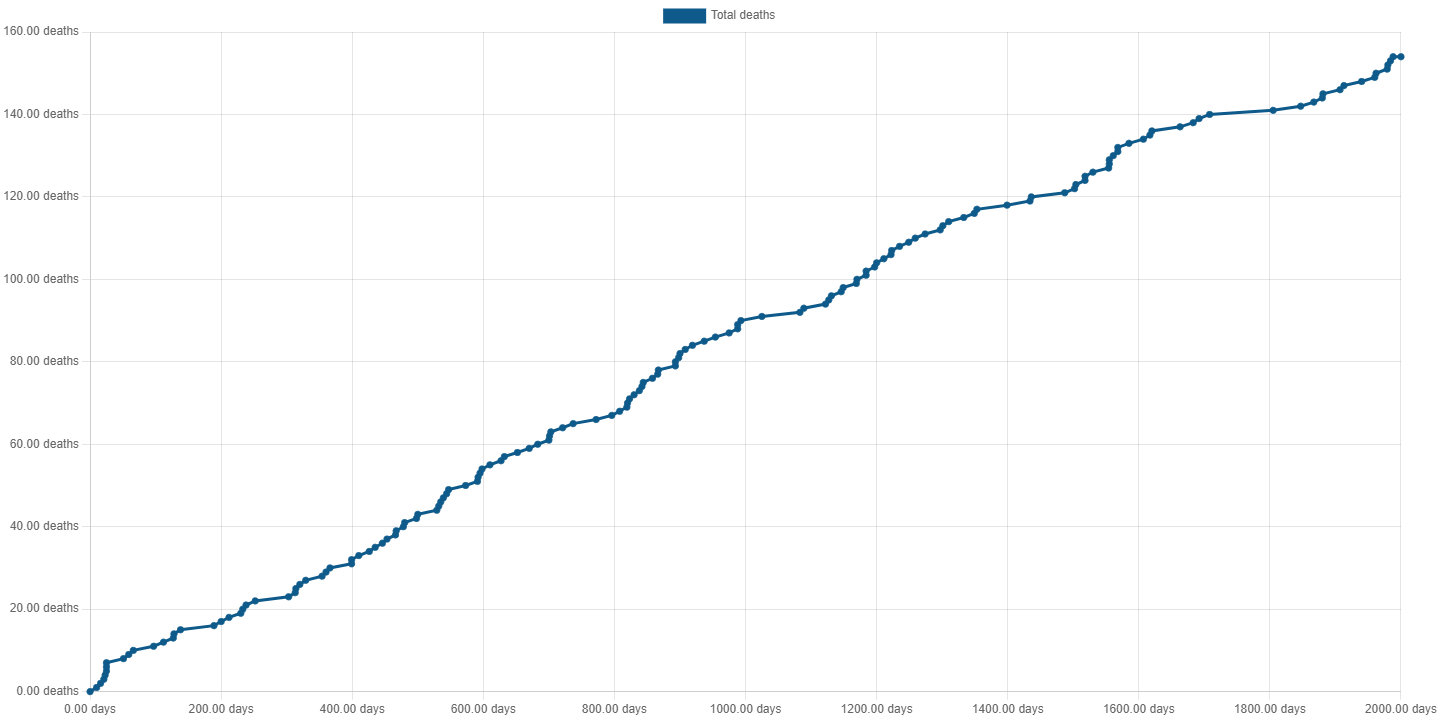
\includegraphics[scale=0.25]{009_team_7_agent_design/Images/Cumulative Deaths, With Treaties, T7Only, 2000days, 20food, High Neur, 154deaths.png}
    \end{center}
    \caption{Cumulative deaths with high neuroticism (154 deaths).}
    \label{fig: High Neuroticism}
\end{figure}

\begin{figure}[H]
    \begin{center}
        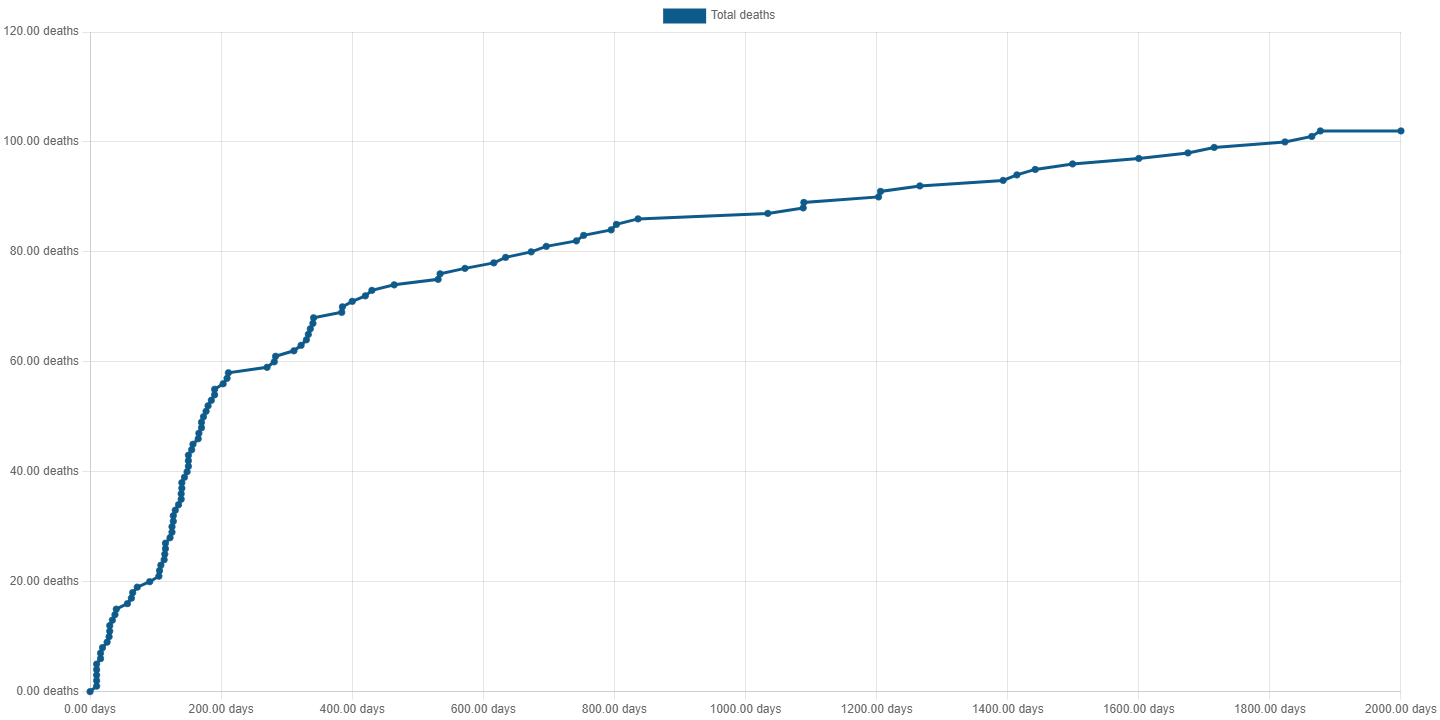
\includegraphics[scale=0.25]{009_team_7_agent_design/Images/Cumulative Deaths, With Treaties, T7Only, 2000days, 20food, Low Neur, 102deaths.png}
    \end{center}
    \caption{Cumulative deaths with low neuroticism (102 deaths).}
    \label{fig: Low Neuroticism}
\end{figure}

It can be seen that higher levels of neuroticism result in a greater number of agent deaths. This is expected as neuroticism results in volatility in an agents behaviour. 

\newpage
\subsubsection{Conscientiousness}
\label{subsubsec: Conscientiousness}

\Cref{fig: High Conscientiousness} and \Cref{fig: Low Conscientiousness} illustrate the results from simulations with agents with high conscientiousness ($>$70) and low conscientiousness ($<$30) respectively. All other traits are left as default.

\begin{figure}[H]
    \begin{center}
        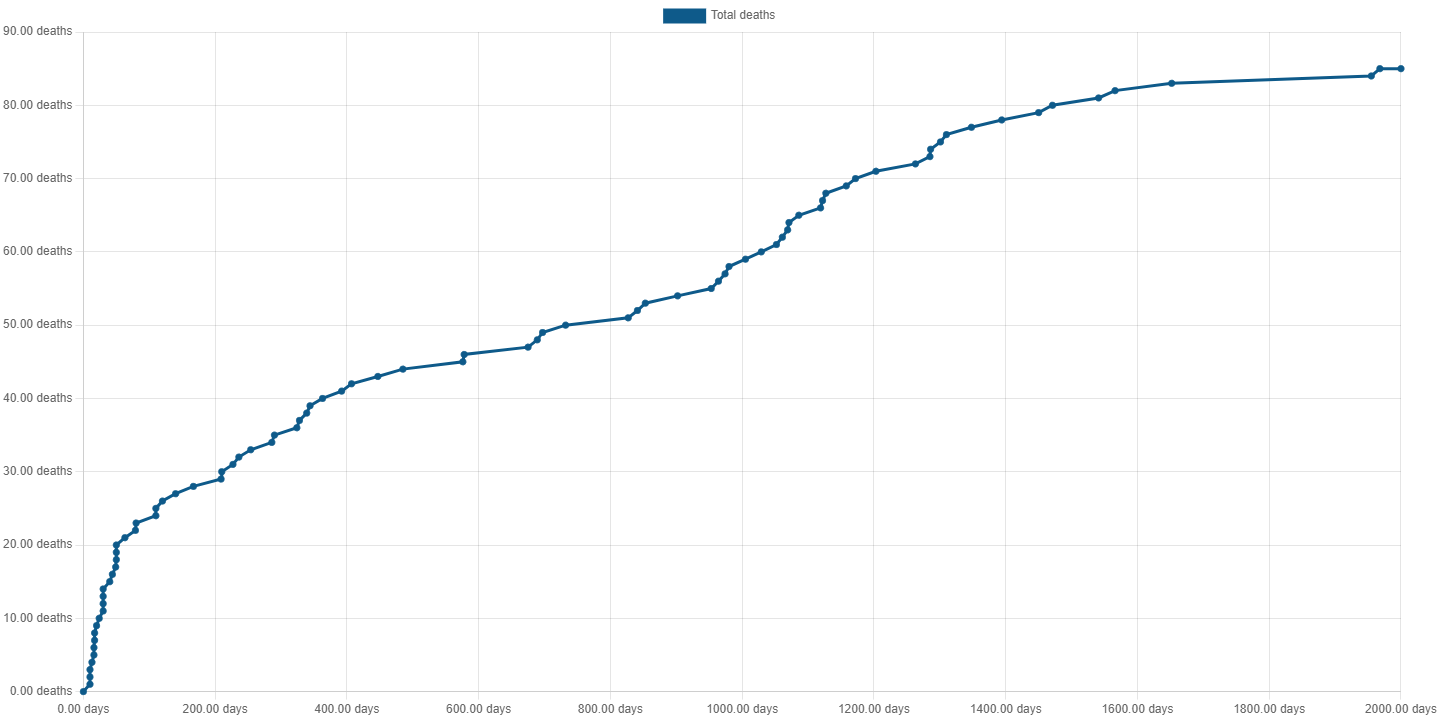
\includegraphics[scale=0.25]{009_team_7_agent_design/Images/Cumulative Deaths, With Treaties, T7Only, 2000days, 20food, High Conscient, 85deaths.png}
    \end{center}
    \caption{Cumulative deaths with high conscientiousness (85 deaths).}
    \label{fig: High Conscientiousness}
\end{figure}

\begin{figure}[H]
    \begin{center}
        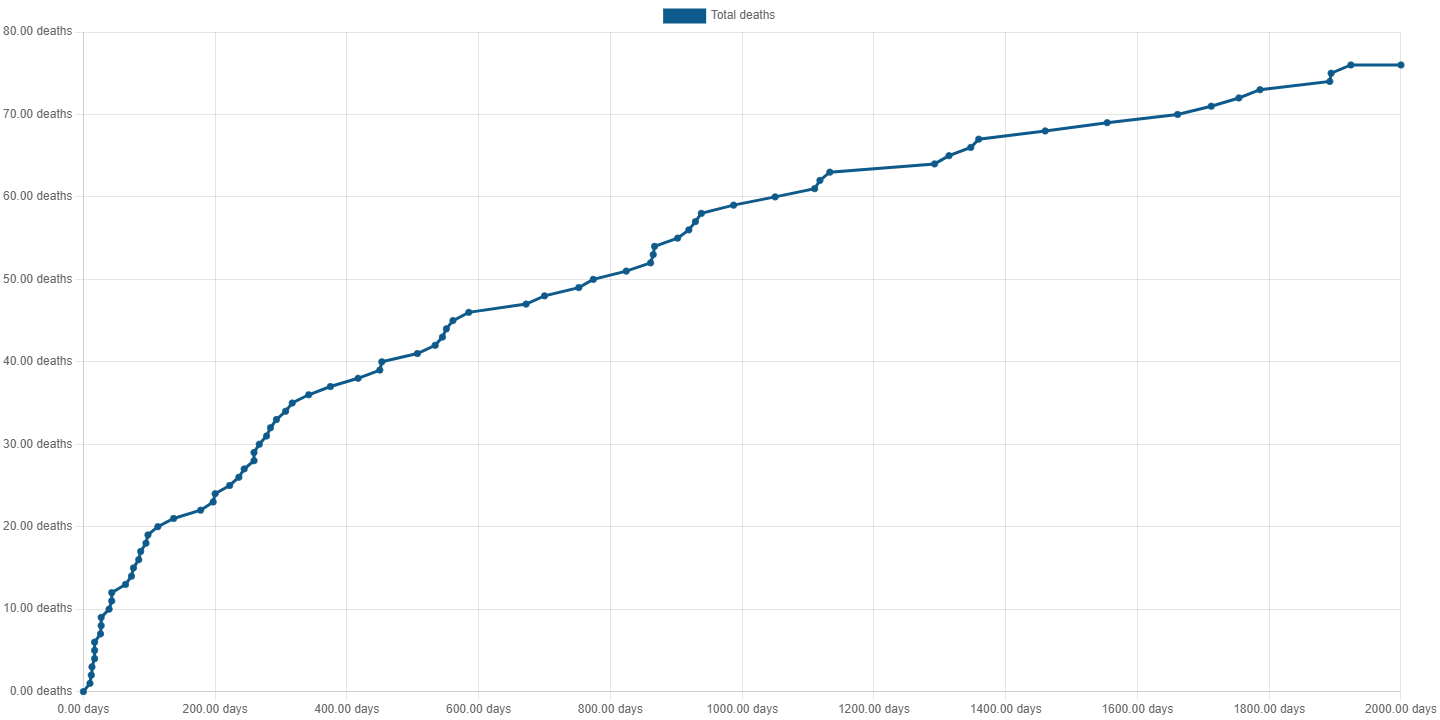
\includegraphics[scale=0.25]{009_team_7_agent_design/Images/Cumulative Deaths, With Treaties, T7Only, 2000days, 20food, Low Conscient, 76deaths.png}
    \end{center}
    \caption{Cumulative deaths with low conscientiousness (76 deaths).}
    \label{fig: Low Conscientiousness}
\end{figure}

It can be observed that there is no substantial difference in the number of deaths when the conscientiousness levels of the agents are collectively varied. This may indicate that the agent struggles to be strategic and that simply being more greedy can be a more effective route to survival. Ultimately, it would appear that other factors outweigh the impact of this personality trait. This is not entirely unreasonable as other personality traits may be more relevant to the given scenario. However, the expectation would be for deaths to reduce with higher conscientiousness although this is not generally observed. 

\newpage
\subsubsection{Extraversion}
\label{subsubsec: Extraversion}
\Cref{fig: High Extraversion} and \Cref{fig: Low Extraversion} illustrate the results from simulations with agents with high extraversion ($>$70) and low extraversion ($<$30) respectively. All other traits are left as default.

\begin{figure}[H]
    \begin{center}
        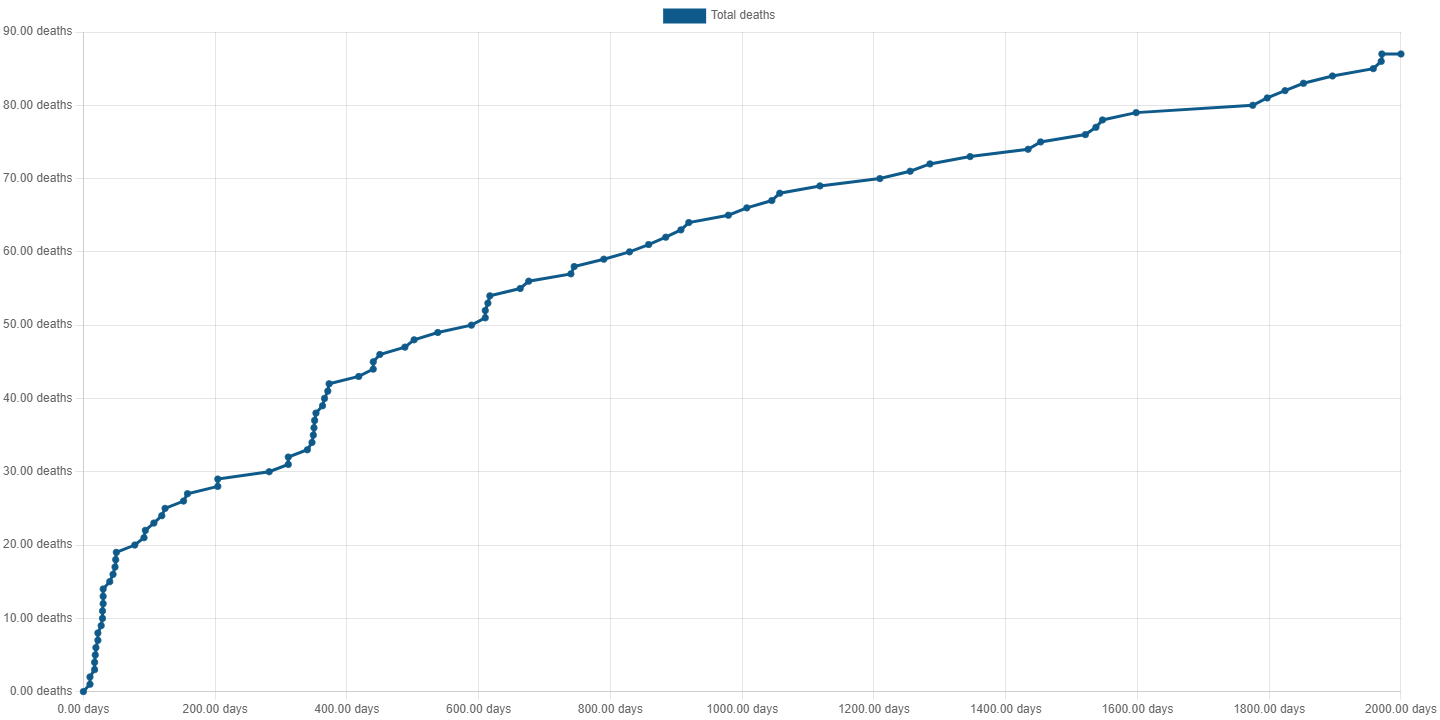
\includegraphics[scale=0.25]{009_team_7_agent_design/Images/Cumulative Deaths, With Treaties, T7Only, 2000days, 20food, High extra, 87deaths.png}
    \end{center}
    \caption{Cumulative deaths with high extraversion (87 deaths).}
    \label{fig: High Extraversion}
\end{figure}

\begin{figure}[H]
    \begin{center}
        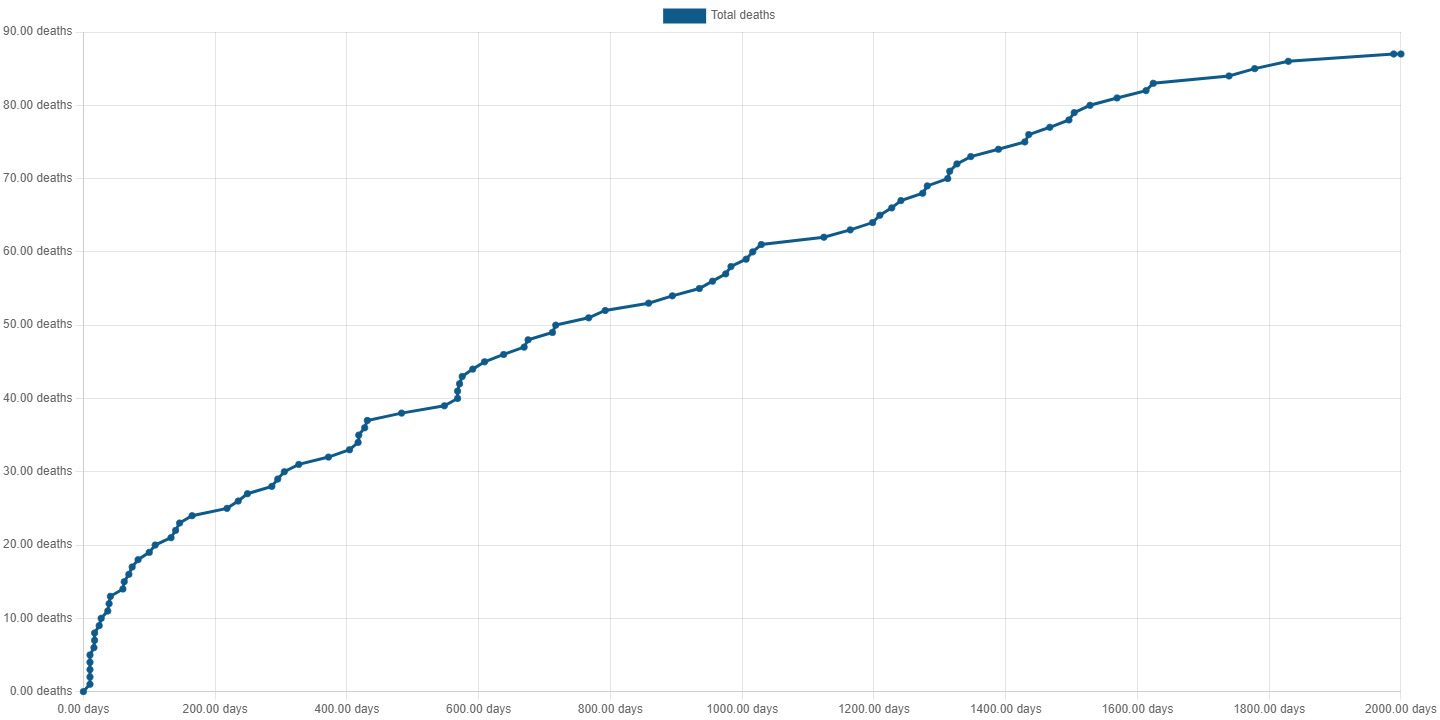
\includegraphics[scale=0.25]{009_team_7_agent_design/Images/Cumulative Deaths, With Treaties, T7Only, 2000days, 20food, Low extra, 87deaths.png}
    \end{center}
    \caption{Cumulative deaths with low extraversion (87 deaths).}
    \label{fig: Low Extraversion}
\end{figure}

Similar to extraversion, simulations show little variation in the number of deaths when the agents' extraversion values are collectively set to either high or low. This may suggest that other factors outweigh the impact of this personality trait. This is not unreasonable as other personality traits may be more relevant to the given scenario. In addition, it is difficult to predict what impact the extraversion level would have on the number of deaths. On one hand, higher extraversion levels will enable a greater number of treaties being signed. On the other hand, it may also result in treaties and requests of lower standards being accepted. These counteractive phenomenon may be the primary cause for the lack of variation in deaths.

\newpage
The following figures explore scenarios where the agents greediness and kindness are fixed before the food taking routine. 

\subsubsection{Greediness}
\label{subsubsec: Greediness}

\Cref{fig: Fixed High Greediness} and \Cref{fig: Fixed Low Greediness} illustrate the results from simulations with agents with high greediness ($>$70) and low greediness ($<$30) respectively. All other traits are left as default.

\begin{figure}[H]
    \begin{center}
        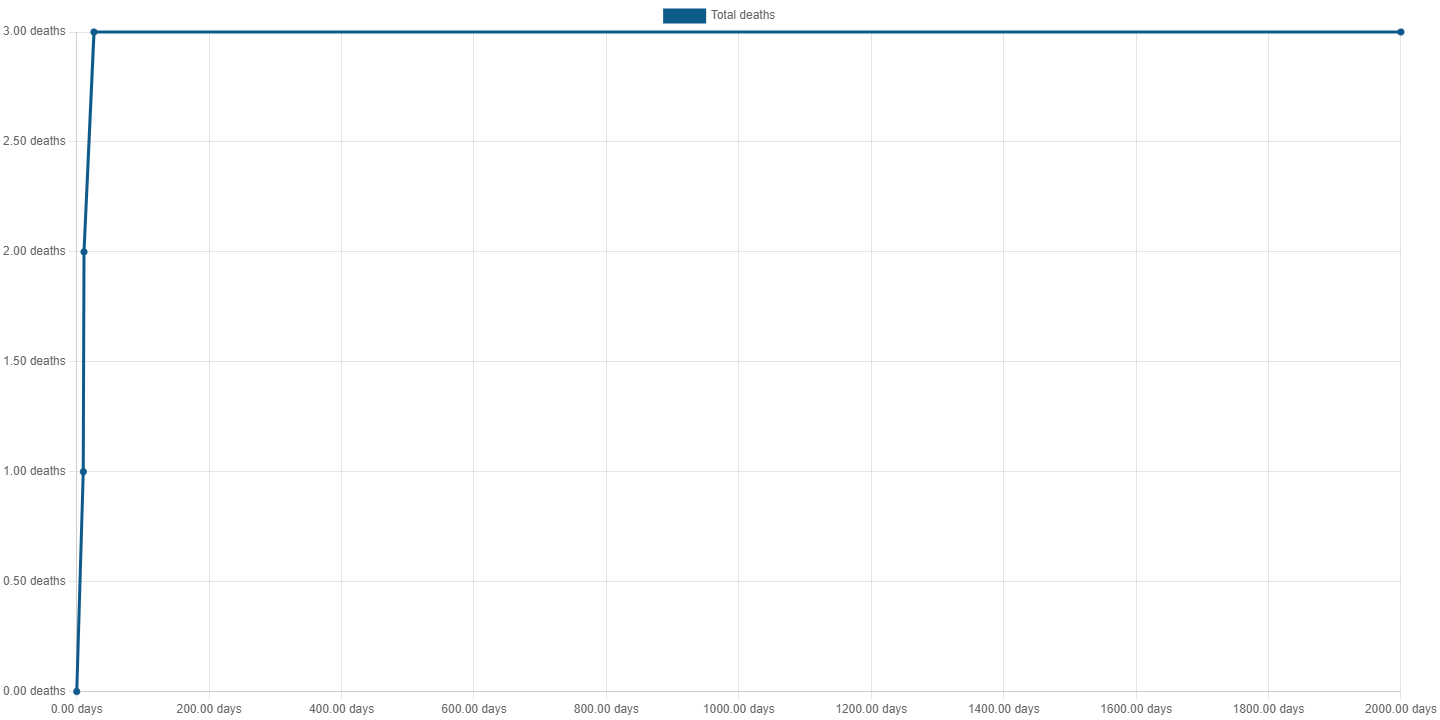
\includegraphics[scale=0.25]{009_team_7_agent_design/Images/Cumulative Deaths, fixed high greediness, T7Only, 2000days, 20food, 3deaths.png}
    \end{center}
    \caption{Cumulative deaths with high greediness (3 deaths).}
    \label{fig: Fixed High Greediness}
\end{figure}

\begin{figure}[H]
    \begin{center}
        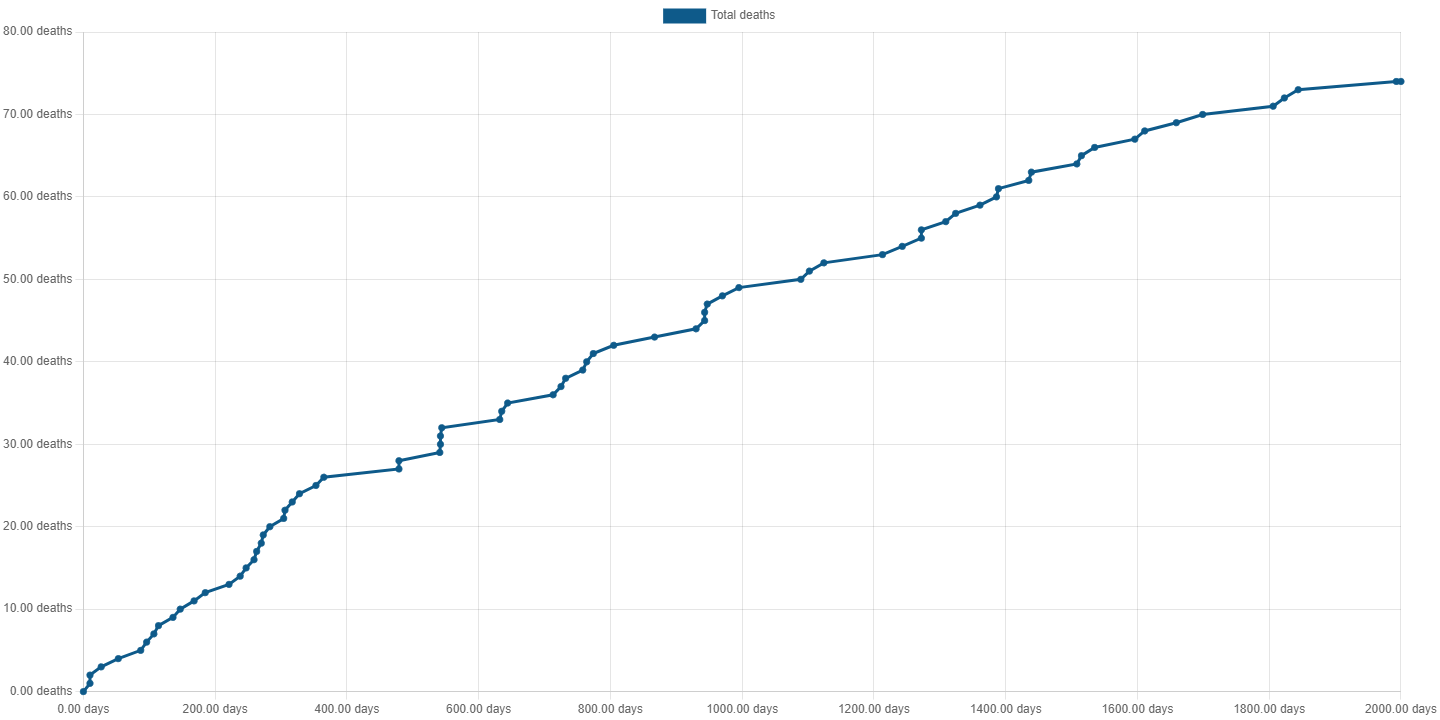
\includegraphics[scale=0.25]{009_team_7_agent_design/Images/Cumulative Deaths, fixed low greediness, T7Only, 2000days, 20food, 74deaths.png}
    \end{center}
    \caption{Cumulative deaths with low greediness (74 deaths).}
    \label{fig: Fixed Low Greediness}
\end{figure}

A tower housing agents with high greediness and enforceable (unbreakable) treaties capabilities show an extremely low death rate suggesting that such a group of agents are able to organise themselves quickly and stabilise the system. A low greediness score sees a dramatic increase in overall deaths and does not achieve stability over the 2000 day simulation.

\subsubsection{Kindness}
\label{subsubsec: Kindness}
\Cref{fig: Fixed High Kindness} and \Cref{fig: Fixed Low Kindness} illustrate the results from simulations with agents with high kindness ($>$70) and low kindness ($<$30) respectively. All other traits are left as default.

\begin{figure}[H]
    \begin{center}
        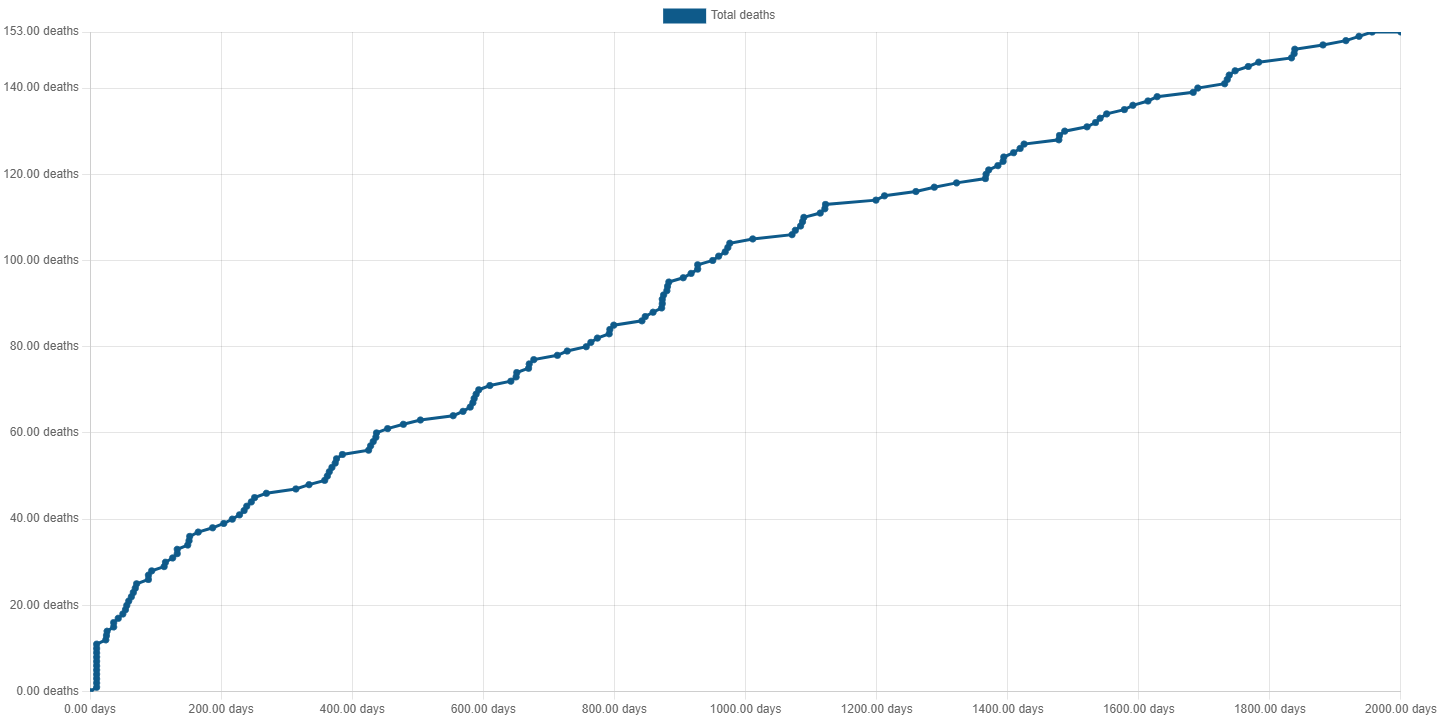
\includegraphics[scale=0.25]{009_team_7_agent_design/Images/Cumulative Deaths, fixed high kindness, T7Only, 2000days, 20food, 153deaths.png}
    \end{center}
    \caption{Cumulative deaths with fixed high kindness (153 deaths).}
    \label{fig: Fixed High Kindness}
\end{figure}

\begin{figure}[H]
    \begin{center}
        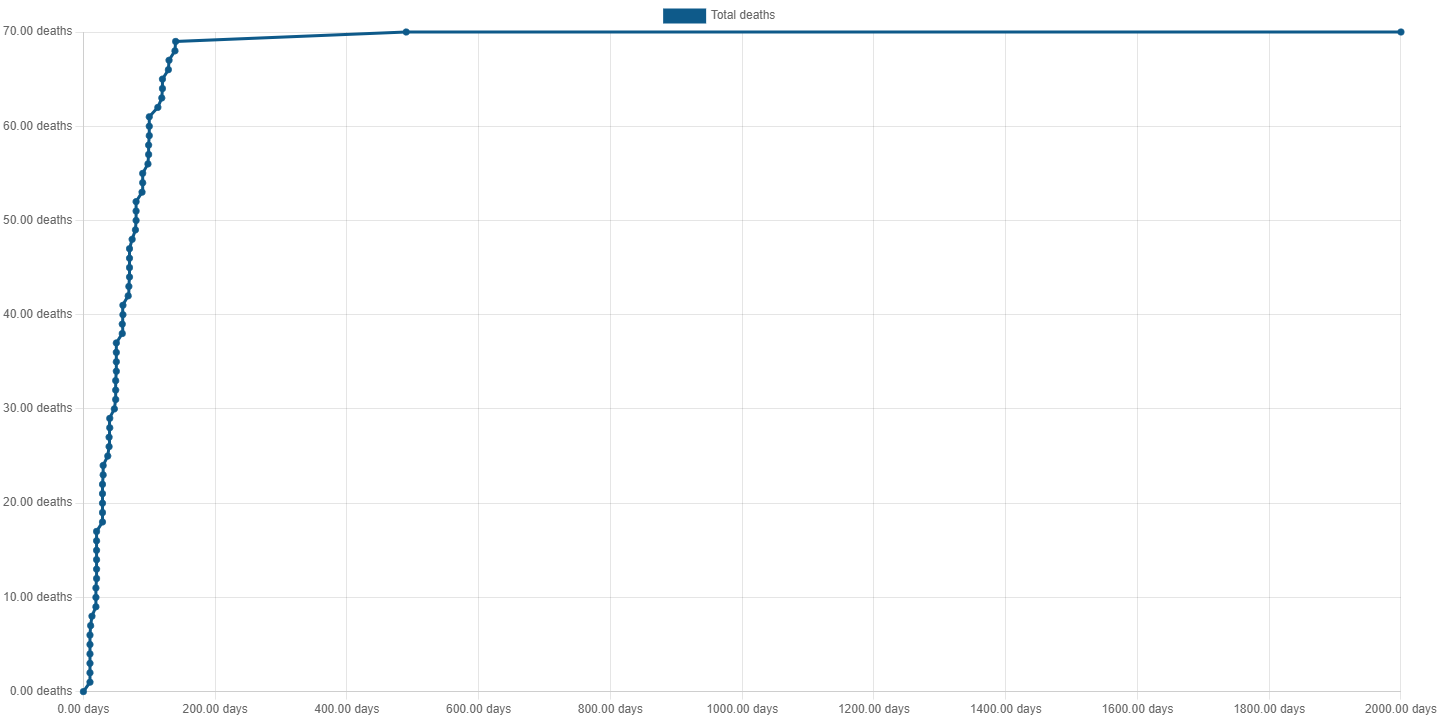
\includegraphics[scale=0.25]{009_team_7_agent_design/Images/Cumulative Deaths, fixed low kindness, T7Only, 2000days, 20food, 70deaths.png}
    \end{center}
    \caption{Cumulative deaths with fixed low kindness (70 deaths).}
    \label{fig: Fixed Low Kindness}
\end{figure}

A high kindness score sees double the deaths of a low kindness score. A high kindness score does not achieve stability however a low kindness score allows for the tower to reach in less than 200. The most likely explanation for this is that agents with a high kindness are potentially too selfless. It is likely that they consume in small quantities when food is available and thus do not have sufficient health when food isn't available. Thus, making them more vulnerable.

\subsubsection{Inter-team Comparison}
\Cref{tab: Inter-team data} shows the total number of deaths for simulations of various combinations of agent teams. All simulations are run with a simulation period of 500 days, shuffle period of 7 days and 10 team 7 agents with 10 agents of one other team type. The table is further broken down into food available per agent (5, 10 and 15).

\begin{table}
    \begin{center}
    \begin{tabular} { | m{4em} | m{6em} | m{4em} | m{4em} | m{4em} | }
      \hline
        \textbf{Agent Team} & \textbf{Food/Agent} & \textbf{Total Deaths} & \textbf{Team 7 Deaths} & \textbf{Other Deaths} \\
      \hline
        2 & 5 & 463 & 273 & 190 \\
      \hline
        2 & 10 & 149 & 80 & 49 \\
      \hline
        2 & 15 & 0 & 0 & 0 \\
      \hline
        3 & 5 & 347 & 183 & 164\\
      \hline
        3 & 10 & 73 & 53 & 20\\
      \hline
        3 & 15 & 0 & 0 & 0 \\
      \hline
        4 & 5 & 217 & 92 & 125\\
      \hline
        4 & 10 & 0 & 0 & 0 \\
      \hline
        4 & 15 & 0 & 0 & 0 \\
      \hline
        5 & 5 & 213 & 107 & 106 \\
      \hline
        5 & 10 & 5 & 5 & 0 \\
      \hline
        5 & 15 &  0 & 0 & 0 \\ 
      \hline
        6 & 5 & 459 & 136 & 323\\
      \hline
        6 & 10 & 273 & 48 & 225\\
      \hline
        6 & 15 & 126 & 24 & 102\\
      \hline
    \end{tabular}
    \end{center}
    \caption{Comparison between agent teams and team 7}
    \label{tab: Inter-team data}
\end{table}

All team agents, bar team 6, were able to coexist with team 7 and achieve zero deaths for a food availability of 15 per agent, indicating that Team 6 agent was the most incompatible with our agent. Team 4 achieved zero deaths for food availability of 10 demonstrating a greater compatibility with team 7 and team 5's results are not too dissimilar.  

\subsubsection{Conclusion}
The agent designed by team 7 is unique in terms of the use of personalities to determine the general behaviour of the agent. These personality traits assigned allow it to mimic human behaviour as much as possible. The results presented above show that the team 7 can have a vastly different behaviours with each other agent, showing our compatibility with some agents and incompatibility with others. In short, the team 7 agent has been intricately designed to meaningfully engage in a huge variety of scenarios and attempt to accomplish its to major goals, to survive individually and collectively.
\chapter{Experiments}\label{experiments}

\section{Overall Aims}
\label{sec: Overall Aims}
The aim of the broader experimentation was to see how the agents behaved in an environment in which they all lived and interacted together and to see what changed when disruptive agents were introduced.
Several independent variables were considered for each experiment, each of which is detailed in the following sections.
The main dependent variable that will be considered is the death rate which determines the system stability. We also sought to observe the dependency on self organisation to achieve stability and the effect of treaties and cooperation on self organisation. Therefore, another important dependent variable that was measured was the number of treaties accepted and rejected by agents.

\section{Disruptive Agents}
\label{sec: Disruptive Agents}
The disruptive agents to be used in the following experiments were a random agent and a selfish agent. They have the following behaviours:
\begin{itemize}
    \item Random Agent: Takes random amounts of food every tick.
    \item Selfish Agent: Takes food every tick such that it always stays at maximum health.
\end{itemize}

\section{Stability}
\label{sec: Stability}
Before the effect of the parameters on stability can be measured, we must first define system stability. The following definition is derived from Ross Ashby’s book, Design for a Brain \cite{Ashby1960}.
Stability is defined in the book as:  “In all cases, the stable system is characterised by the fact that after a displacement we can assign some bound to the subsequent movement of the representative (equilibrium) point.”
The features of a system's stability as given by \cite{Ashby1960} are as follows:
\begin{itemize}
    \item Stability refers to some aspect of a system, not the system itself.
    \item A stable system is brought back to a state of equilibrium when it is displaced.
    \item Stability is a property of the whole system.
    \item Presence of stability implies some coordination of actions of the parts.
\end{itemize}
 
In the case of the tower as a system, the death rate is considered to be the equilibrium point and the displacement being the addition of agents to the tower since, before the introduction of the agents, there is no movement in any of the parameters of the system. The equilibrium point being a death rate of zero. 

The tower can therefore be considered stable if:
\begin{itemize}
    \item The death rate reaches zero
    \item The death rate stays at zero for at least one reshuffle period
    \item The death rate stays at zero until the end of the simulation
\end{itemize}
 
This definition of tower stability also has the four features mentioned above and in the book.

\section{Experiment 1}
\label{sec: Experiment 1}
\subsection{Aims}
\label{subsec: E1-Aims}
The aim of this experiment is to observe the impact of the addition of disruptive agents on the tower. 
We keep an equal number of each team’s agents in the tower. Selfish agents and random agents are then added. The food per agent on the platform (food scarcity) is also varied. This allows us to observe the effect of food scarcity on stability and the effect of the addition of these disruptive agents on tower stability. Of course, we expect that as food becomes more scarce and as more disruptive agents are added, the total number of deaths will increase and stability will be more difficult to achieve.

In this experiment the tower being used is highly heterogeneous, with 3 of each team agent type being added to it. Three random agents, three selfish agents or three of both or none of either will then be added to to the tower.
\subsection{Results and Discussion}
\label{subsec: E1-Results and Discussion}

\begin{figure}[H] %Treaties Rejected As Food Scarcity Decreases
    \centering
    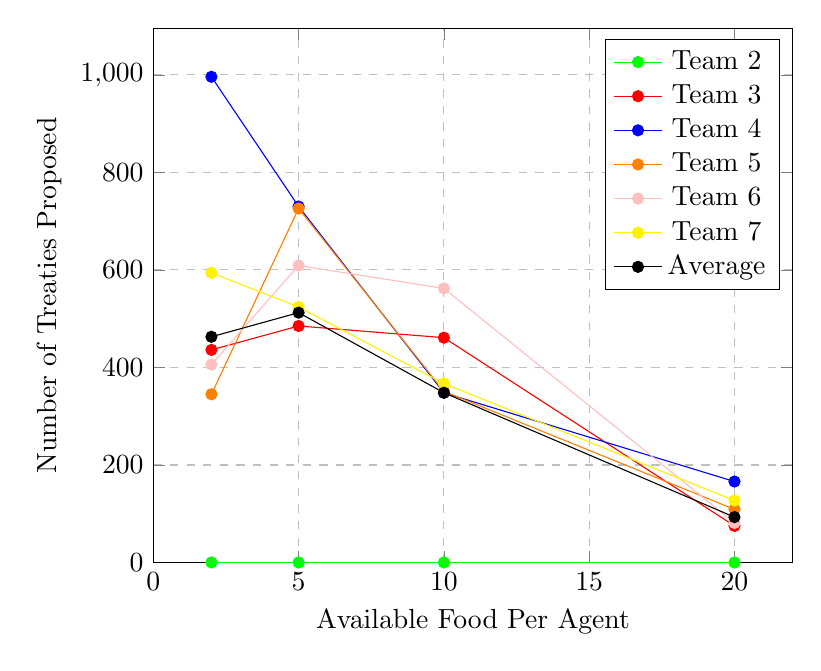
\begin{tikzpicture}
        \begin{axis}[
            width=0.8\textwidth,
            % axis y line*=left,
            ymin=0,
            xmin=0,
            xlabel=Available Food Per Agent,
            ylabel=Number of Treaties Proposed,
            ymajorgrids=true,
            xmajorgrids=true,
            grid style=dashed,
        ]
        \addplot[mark=*,green]
            coordinates{
                (2, 0)
                (5, 0)
                (10, 0)
                (20, 0)
            }; \label{leg:team2-scarcity}
        \addplot[mark=*,red]
            coordinates{
                (2, 436)
                (5, 485)
                (10, 461)
                (20, 75)
            }; \label{leg:team3-scarcity}
        \addplot[mark=*,blue]
            coordinates{
                (2, 996)
                (5, 730)
                (10, 348)
                (20, 166)
            }; \label{leg:team4-scarcity}
        \addplot[mark=*,orange]
            coordinates{
                (2, 345)
                (5, 726)
                (10, 351)
                (20, 109)
            }; \label{leg:team5-scarcity}
        \addplot[mark=*,pink]
            coordinates{
                (2, 406)
                (5, 609)
                (10, 562)
                (20, 81)
            }; \label{leg:team6-scarcity}
        \addplot[mark=*,yellow]
            coordinates{
                (2, 594)
                (5, 524)
                (10, 367)
                (20, 127)
            }; \label{leg:team7-scarcity}
        \addplot[mark=*,black]
            coordinates{
                (2, 462.83)
                (5, 512.33)
                (10, 348.17)
                (20, 93)
            }; \label{leg:average-scarcity}
        \addlegendimage{/pgfplots/refstyle=leg:team2-scarcity}\addlegendentry{Team 2}
        \addlegendimage{/pgfplots/refstyle=leg:team3-scarcity}\addlegendentry{Team 3}
        \addlegendimage{/pgfplots/refstyle=leg:team4-scarcity}\addlegendentry{Team 4}
        \addlegendimage{/pgfplots/refstyle=leg:team5-scarcity}\addlegendentry{Team 5}
        \addlegendimage{/pgfplots/refstyle=leg:team6-scarcity}\addlegendentry{Team 6}
        \addlegendimage{/pgfplots/refstyle=leg:team7-scarcity}\addlegendentry{Team 7}
        \addlegendimage{/pgfplots/refstyle=leg:average-scarcity}\addlegendentry{Average}
        \end{axis}
        \end{tikzpicture}
    \caption{Number of Treaties Proposed as Food Scarcity Decreases}
    \label{fig:team1-robustness-food-scarcity}
\end{figure}

\Cref{fig:team1-robustness-food-scarcity} illustrates the change in the frequency of treaty proposal as the constraints from the economy of scarcity are levied. The experiment enforces that there is 100 food initially available on the platform, with the number of agents parameterised to allow for an average amount of food per agent. This simulation lasts 400 turns.

The general tendency for this system is that, as the availability of food rises (and hence the economy of scarcity becomes less constrictive), the rate of treaty proposal decreases. We propose that this experiment yields insight into the importance of treaties, demonstrating that agents in general rely heavily on treaty formation to self organise when survivability is hindered by a lack of resources. On the contrary, as the food availability reaches an abundance, we see the rate of treaty proposal tend to 0, suggesting that agents are able to survive without the need for treaties as they offer little utility.

We also assert that this graph details the implied benefit of signing treaties: agents seem to value treaties as a means to fairer food distribution, wherein signing facilitates them receiving a greater proportion of food than they would otherwise receive without a treaty.

\begin{figure}[H] %Deaths As Food Scarcity Decreases with different agent combos added
    \centering
    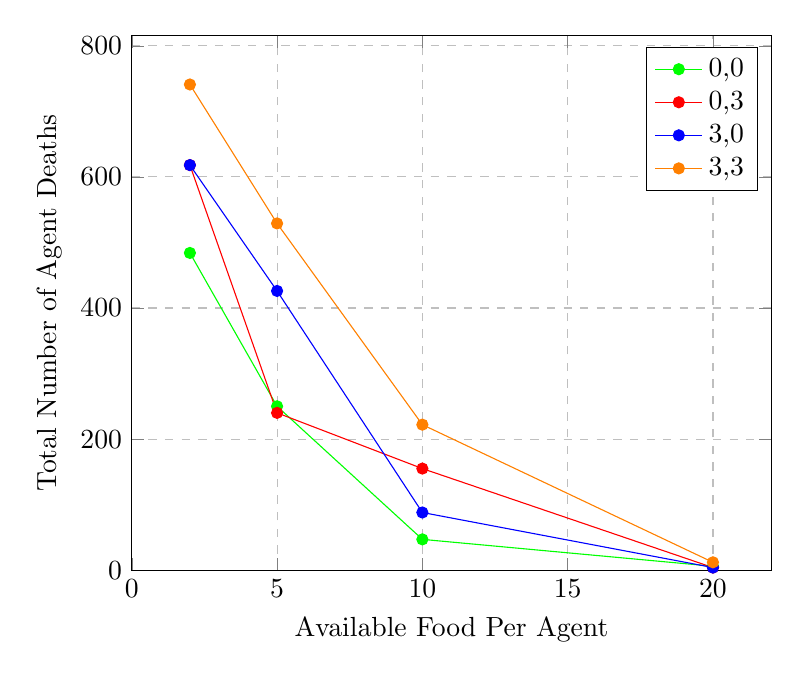
\begin{tikzpicture}
        \begin{axis}[
            width=0.8\textwidth,
            % axis y line*=left,
            ymin=0,
            xmin=0,
            xlabel=Available Food Per Agent,
            ylabel=Total Number of Agent Deaths,
            ymajorgrids=true,
            xmajorgrids=true,
            grid style=dashed,
        ]
        \addplot[mark=*,green]
            coordinates{
                (2, 484)
                (5, 250)
                (10, 47)
                (20, 6)
            }; \label{leg:scarcity00}
        \addplot[mark=*,red]
            coordinates{
                (2, 618)
                (5, 240)
                (10, 155)
                (20, 4)
            }; \label{leg:scarcity03}
        \addplot[mark=*,blue]
            coordinates{
                (2, 618)
                (5, 426)
                (10, 88)
                (20, 4)
            }; \label{leg:scarcity30}
        \addplot[mark=*,orange]
            coordinates{
                (2, 741)
                (5, 529)
                (10, 222)
                (20, 12)
            }; \label{leg:scarcity33}
        \addlegendimage{/pgfplots/refstyle=leg:scarcity00}\addlegendentry{0,0}
        \addlegendimage{/pgfplots/refstyle=leg:scarcity03}\addlegendentry{0,3}
        \addlegendimage{/pgfplots/refstyle=leg:scarcity30}\addlegendentry{3,0}
        \addlegendimage{/pgfplots/refstyle=leg:scarcity33}\addlegendentry{3,3}
        \end{axis}
        \end{tikzpicture}
    \caption{The total number of deaths in systems with different combinations of selfish and random agents added as food per agent increases. The number of each disruptive agent added to each system is show in the legend in the form (number of selfish agents, number of random agents)}
    \label{fig:team1-robustness-food-scarcity-disruptive-agents}
\end{figure}

\Cref{fig:team1-robustness-food-scarcity-disruptive-agents} shows how the number of deaths is affected when different disruptive agents are added. It shows that, as expected, the number of deaths is higher when disruptive agents are present. However, the effect of selfish agents and random agents seem to be similar which suggests that it it not the amount of food being taken by the agents that is disruptive, rather it is the fact that they do not communicate that causes a higher death rate. This makes it harder to self organise and makes it much harder to survive in the tower. 
And by making it harder to survive in the tower, the chances of reaching a stable system are also decreased when disruptive agents are added, the only system to stabilise with 10 food per agent was the one with no disruptive agents, all systems were stable with a tower of 20 food per agent.
\subsection{Conclusion}
\label{subsec: E1-Conclusion}
This experiment shows the importance of treaties and communication for the survival of the agents in the tower. This implies that self organisation is a key factor in the ability of the tower to reach a stable state.

\section{Experiment 2}
\label{subsec: Experiment 2}
\subsection{Aims}
\label{subsec: E2-Aims}
The aim of this experiment is to vary the number of ticks per floor and reshuffle period and observe the effects of this on tower stability and ability to self organise.
\subsection{Results and Discussion}
\label{subsec: E2-Results and Discussion}

\begin{figure}[H] %Number of Deaths As Shuffle Period Decreases
    \centering
    \begin{minipage}{0.8\textwidth}
        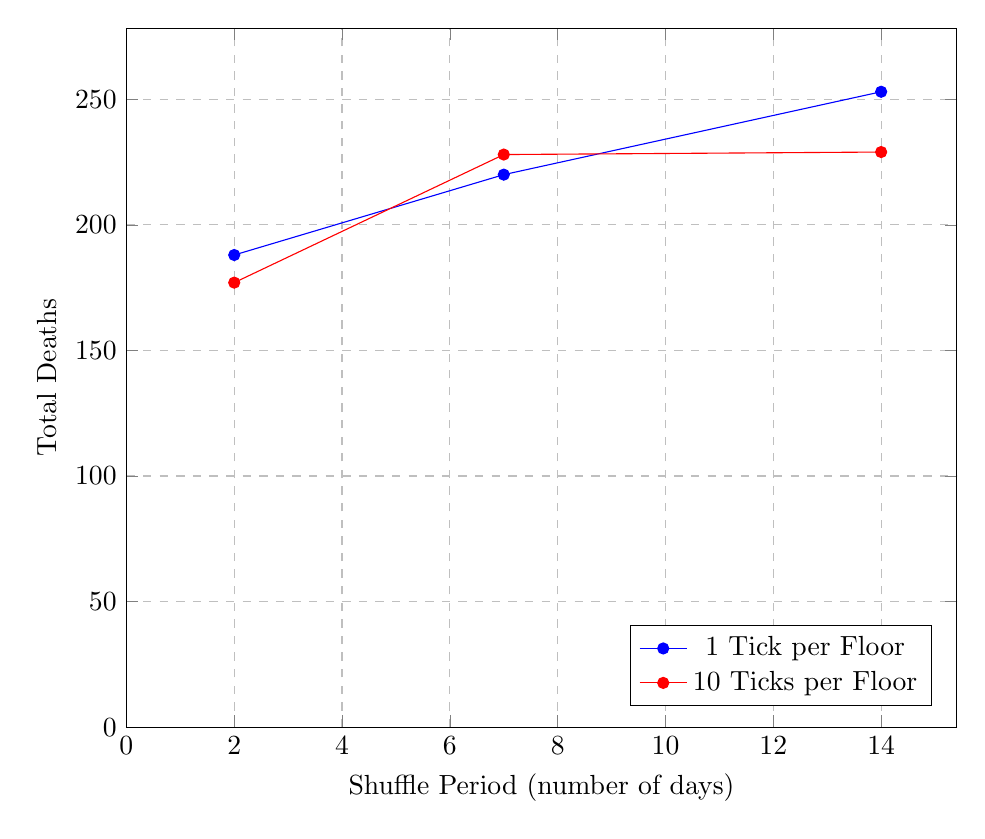
\begin{tikzpicture}
            \begin{axis}[
                width=\textwidth,
                % axis y line*=left,
                ymin=0,
                xmin=0,
                xlabel=Shuffle Period (number of days),
                ylabel=Total Deaths,
                ymajorgrids=true,
                xmajorgrids=true,
                grid style=dashed,
                legend pos=south east
            ]
            \addplot[mark=*,blue]
                coordinates{
                    (14, 253)
                    (7, 220)
                    (2, 188)
                }; \label{leg:reshuffle-ticks-per-floor1}
            \addplot[mark=*,red]
                coordinates{
                    (14, 229)
                    (7, 228)
                    (2, 177)
                }; \label{leg:reshuffle-ticks-per-floor10}
            \addlegendimage{/pgfplots/refstyle=leg:reshuffle-ticks-per-floor1}
            \addlegendentry{1 Tick per Floor}
            \addlegendimage{/pgfplots/refstyle=leg:reshuffle-ticks-per-floor10}\addlegendentry{10 Ticks per Floor}
            \end{axis}
        \end{tikzpicture}
    \end{minipage}
    \caption{Total Deaths in the Tower as Reshuffle Period Increases}
    \label{fig:Number-of-Deaths-As-Shuffle-Period-Decreases}
\end{figure}


For this reason, we propose that it is the rapid redistribution of agents throughout the tower, allowing them to experience varying levels of available food that accounts for the disparity in survival rate: if an agent is consistently assigned to a low floor, they have a low chance of being satisficed if all agents act individually. Having a rapid reshuffle period results in a higher probability of reaching a higher floor, allowing for the agent to replenish its health. 

The average age of agents, denoted by \Cref{fig:Average-Age-as-Shuffle-Period-Decreases}, can be see to follow the inverse trend to death rates which is as expected. This trend being, that the longer the reshuffle period the lower the average age of an agent at death. 
\begin{figure}[H] %Average Age As Shuffle Period Decreases
    \centering
    \begin{minipage}{0.8\textwidth}
        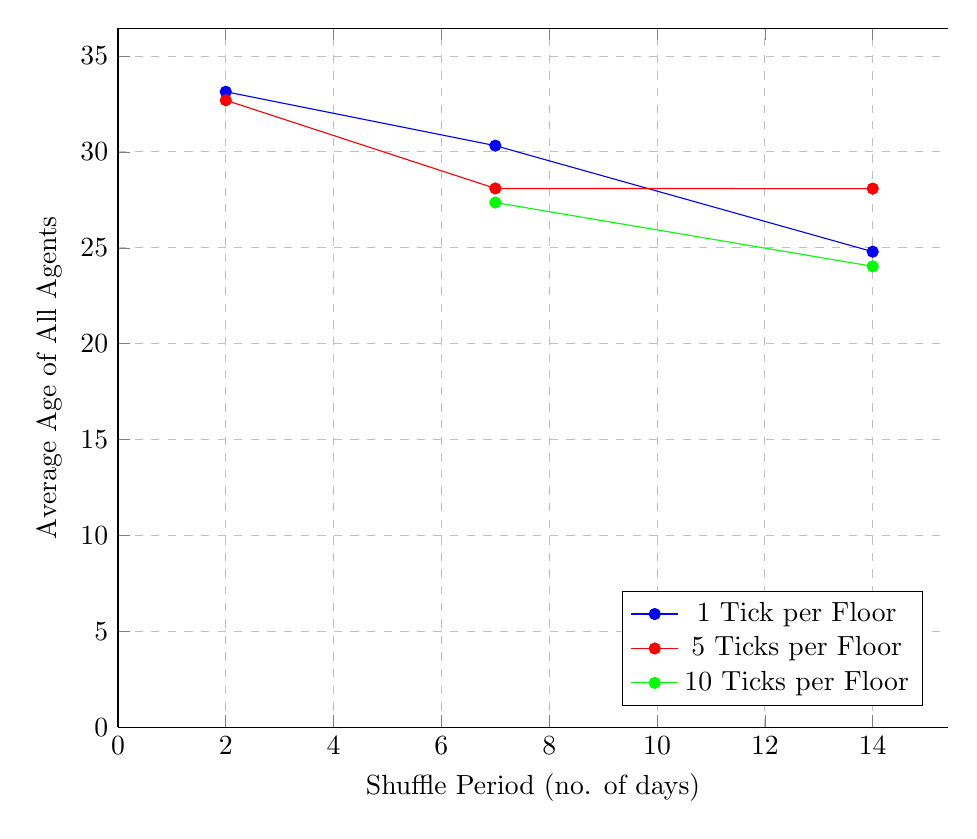
\begin{tikzpicture}
            \begin{axis}[
                width=\textwidth,
                axis y line*=left,
                ymin=0,
                xmin=0,
                xlabel=Shuffle Period (no. of days),
                ylabel=Average Age of All Agents,
                ymajorgrids=true,
                xmajorgrids=true,
                grid style=dashed,
                legend pos=south east
            ]
            \addplot[mark=*,blue]
                coordinates{
                    (14, 24.798)
                    (7, 30.327)
                    (2, 33.138)
                }; \label{leg:reshuffle-ticks-per-floor1}
            \addplot[mark=*,red]
                coordinates{
                    (14, 28.087)
                    (7, 28.096)
                    (2, 32.695)
                }; \label{leg:reshuffle-ticks-per-floor10}
            \addplot[mark=*,green]
                coordinates{
                    (14, 24.034)
                    (7, 27.36)
                }; \label{leg:reshuffle-ticks-per-floor5}
            \addlegendimage{/pgfplots/refstyle=leg:reshuffle-ticks-per-floor1}
            \addlegendentry{1 Tick per Floor}
            \addlegendimage{/pgfplots/refstyle=leg:reshuffle-ticks-per-floor5}
            \addlegendentry{5 Ticks per Floor}
            \addlegendimage{/pgfplots/refstyle=leg:reshuffle-ticks-per-floor10}\addlegendentry{10 Ticks per Floor}
            \end{axis}
        \end{tikzpicture}
    \end{minipage}
    \caption{Average Age in the Tower as Reshuffle Period Increases}
    \label{fig:Average-Age-as-Shuffle-Period-Decreases}
\end{figure}

\Cref{fig:Total-Accepted-Treaties-As-Shuffle-Period-Decreases} and \Cref{fig:Total-Rejected-Treaties-As-Shuffle-Period-Decreases} show that significant numbers of treaties are being exchanged at all reshuffle periods, demonstrating that a social network is being formed. However, as the reshuffle period decreases the number of treaties accepted and rejected, the total number of treaties proposed also decreases. This is as expected since, if agents have the same neighbours for longer periods of time, they need to exchange fewer new treaties, given that each proposed treaty will be agreed upon by neighbours for longer and so neighbours will not need to send each other new treaties. 

\begin{figure}[H] %Total Accepted Treaties As Shuffle Period Decreases
    \centering
    \begin{minipage}{0.8\textwidth}
        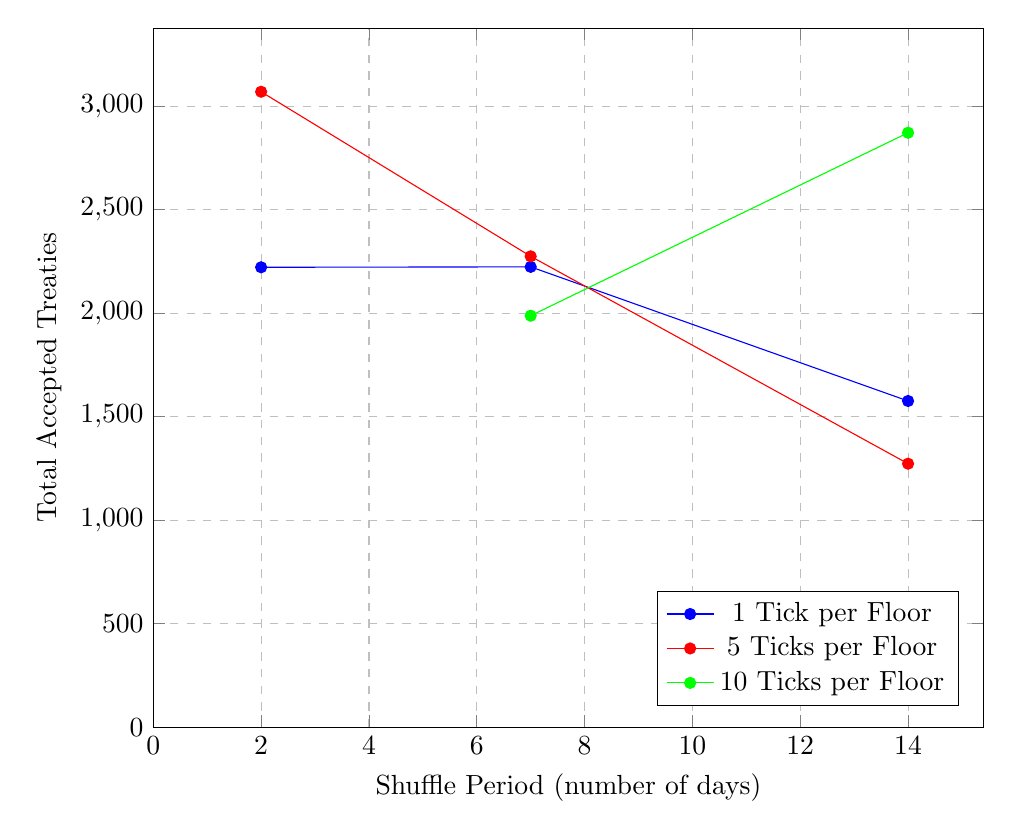
\begin{tikzpicture}
            \begin{axis}[
                width=\textwidth,
                % axis y line*=left,
                ymin=0,
                xmin=0,
                xlabel=Shuffle Period (number of days),
                ylabel=Total Accepted Treaties,
                ymajorgrids=true,
                xmajorgrids=true,
                grid style=dashed,
                legend pos=south east
            ]
            \addplot[mark=*,blue]
                coordinates{
                    (14, 1576)
                    (7, 2224)
                    (2, 2222)
                }; \label{leg:reshuffle-ticks-per-floor1}
            \addplot[mark=*,red]
                coordinates{
                    (14, 1273)
                    (7, 2275)
                    (2, 3070)
                }; \label{leg:reshuffle-ticks-per-floor10}
            \addplot[mark=*,green]
                coordinates{
                    (14, 2872)
                    (7, 1988)
                }; \label{leg:reshuffle-ticks-per-floor5}
            \addlegendimage{/pgfplots/refstyle=leg:reshuffle-ticks-per-floor1}
            \addlegendentry{1 Tick per Floor}
            \addlegendimage{/pgfplots/refstyle=leg:reshuffle-ticks-per-floor5}
            \addlegendentry{5 Ticks per Floor}
            \addlegendimage{/pgfplots/refstyle=leg:reshuffle-ticks-per-floor10}\addlegendentry{10 Ticks per Floor}
            \end{axis}
        \end{tikzpicture}
    \end{minipage}
    \caption{Total Accepted Treaties As Shuffle Period Decreases}
    \label{fig:Total-Accepted-Treaties-As-Shuffle-Period-Decreases}
\end{figure}

\begin{figure}[H] %Total Rejected Treaties As Shuffle Period Decreases
    \centering
    \begin{minipage}{0.8\textwidth}
        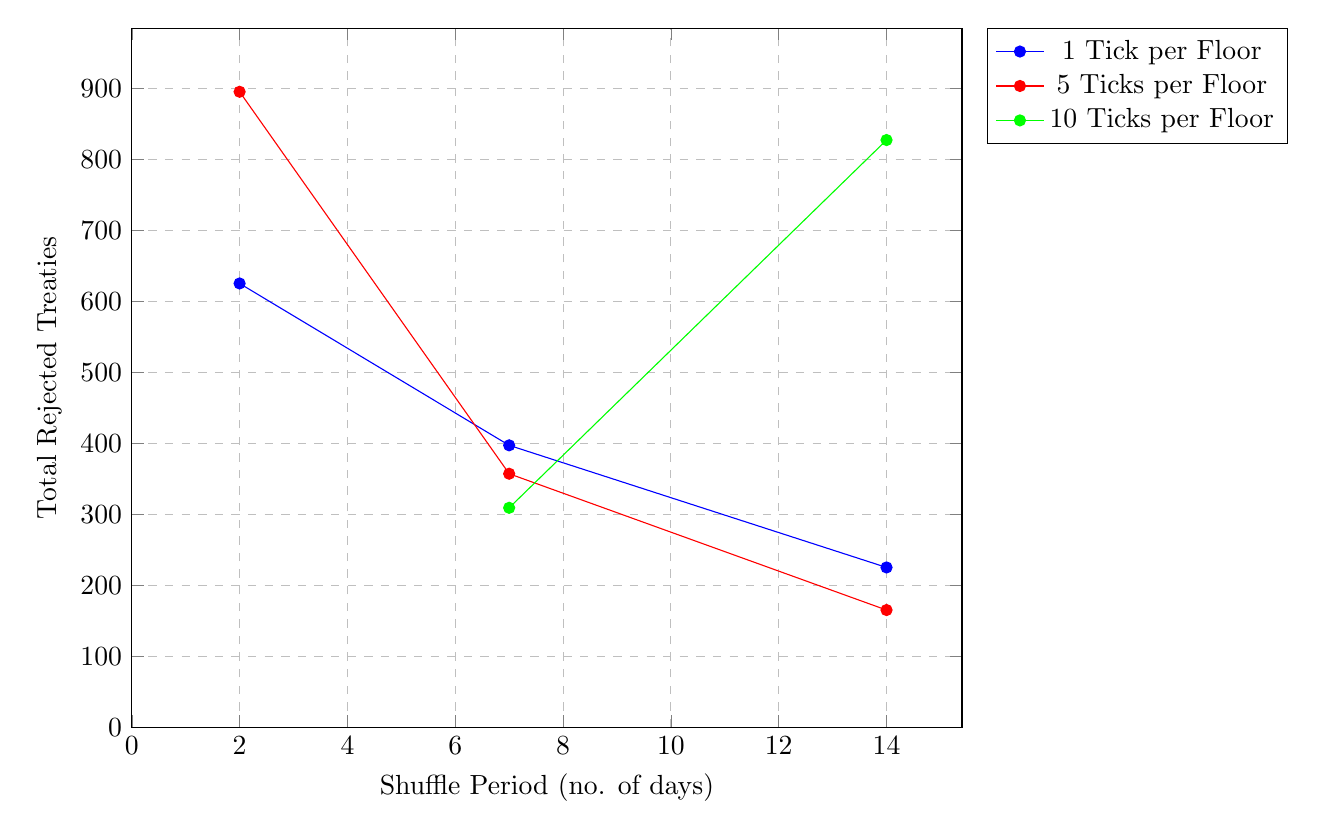
\begin{tikzpicture}
            \begin{axis}[
                width=\textwidth,
                % axis y line*=left,
                ymin=0,
                xmin=0,
                xlabel=Shuffle Period (no. of days),
                ylabel=Total Rejected Treaties,
                ymajorgrids=true,
                xmajorgrids=true,
                grid style=dashed,
                legend pos=outer north east
            ]
            \addplot[mark=*,blue]
                coordinates{
                    (14, 225)
                    (7, 397)
                    (2, 625)
                }; \label{leg:reshuffle-ticks-per-floor1}
            \addplot[mark=*,red]
                coordinates{
                    (14, 165)
                    (7, 357)
                    (2, 895)
                }; \label{leg:reshuffle-ticks-per-floor10}
            \addplot[mark=*,green]
                coordinates{
                    (14, 827)
                    (7, 309)
                }; \label{leg:reshuffle-ticks-per-floor5}
            \addlegendimage{/pgfplots/refstyle=leg:reshuffle-ticks-per-floor1}
            \addlegendentry{1 Tick per Floor}
            \addlegendimage{/pgfplots/refstyle=leg:reshuffle-ticks-per-floor5}
            \addlegendentry{5 Ticks per Floor}
            \addlegendimage{/pgfplots/refstyle=leg:reshuffle-ticks-per-floor10}\addlegendentry{10 Ticks per Floor}
            \end{axis}
        \end{tikzpicture}
    \end{minipage}
    \caption{Total Rejected Treaties As Shuffle Period Decreases}
    \label{fig:Total-Rejected-Treaties-As-Shuffle-Period-Decreases}
\end{figure}

\subsection{Conclusion}
\label{subsec: E2-Conclusion}
The change in reshuffle period and number of ticks per floor does not have a significant impact on the ability of the agents to self organise. However, increasing the reshuffle period does increase the overall deaths and so would make reaching stability more difficult.



\chapter{Results}\label{results}
\chapter{Discussion}\label{discussion}
\chapter{Conclusion}\label{conclusion}

This project has involved the design and implementation of six different agents with various strategies to self-organise and solve a common resource management problem, where the common resource, in this case, is the scarcity of food available to agents in the tower.

It has been shown that in order for self-organisation to be achieved within the tower, communication is necessary between all present agents through both messaging and the signing of treaties. Agents which were succesful in achieving self-organisation did so by gaining knowledge of both the tower and other agents, and applying this knowledge appropriately. Without this, the most logical behaviour of an agent is to act purely selfishly, giving itself the best chance of survival in a random system.
% Appendix
\appendix
\chapter{Project Management}\label{sec:proj-mgmt}

\section{Organisation}
In order to allow for more focused work, the cohort was split into seven teams for this project:
\begin{itemize}
    \item Team 1 was responsible for designing the infrastructure, MVP, and frontend and visualisation tools, with a group size of 9.
    \item Teams 2 to 7 were responsible for designing agent strategies, with group sizes of either 6 or 7.
\end{itemize}
Alongside this, some individual members took on additional organisation and planning roles for the cohort.

Each team had a team lead (except for Team 1, which due to its large size and remit, had two team leads):
\begin{enumerate}
    \item Team 1: Jaafar Rammal and Cyrus Goodarzi
    \item Team 2: Tom Eaton
    \item Team 3: Sara Fernandez
    \item Team 4: Hussain Kurabadwala
    \item Team 5: Jason Zheng
    \item Team 6: Matthew Scott
    \item Team 7: Moin Bukhari
\end{enumerate}
Team leads were responsible for representing the views of their team and communicating information between their team and the wider cohort.

Regular meetings were held between Professor Pitt and the SOMAS cohort to facilitate cohort-wide discussion and feedback.

Any member was free to discuss system features and implement these such as health, message passing, and treaties.

Go was chosen as the programming language with GitHub used for version control.

Communication was done primarily using the communication platform Slack, with some teams choosing to use their own methods of communication such as Discord, Microsoft Teams, and WhatsApp.

\section{Reflection}
No one in the cohort had any experience in writing Go prior to this project; every person who contributed to the codebase learned the language from scratch at the beginning of the project.

Many individuals were also not comfortable with using Git for version control; they have gained a lot more experience in using Git throughout this project.

Our fundamental organisation structure of having agent teams and a separate infrastructure team seemed to work well overall after the MVP was released, with the infrastructure team available to discuss and implement requests for functionality.

There should have been one person who was not assigned to any team designated as the overall project manager. The project management was primarily done by two people who were also team leads and who heavily contributed to discussion and implementation of key features; this meant that they were stretched very thinly across the project and had a workload significantly higher than most other members.

The system design architecture should have been one of the first decisions that we made as a cohort; instead this was done after deciding on programming language and splitting into teams. This turned out to be a mistake as the simulation architecture then became the sole responsibility of the infrastructure team. This is a high-stakes responsibility and as such should have had more involvement from the wider cohort.

There was no enforced requirement for teams to document features and functionality; this made conveying changes to the cohort difficult and would have made writing the report easier.

Furthermore, information about incoming features could have been communicated better; the primary way this was done for this project was by asking people to look at pull requests. This could have instead been done using a document summarising the changes and new APIs.

This report should have been written continuously as the project progressed rather than in the final week.

The role of a team lead should have been more explicitly defined: team leads did not have the same understanding of the role as the project managers did. This contributed to the unbalanced workload among the cohort. Moreover, the introduction of the role of team lead led to a loss of accountability among many members of the cohort who were not team leads and therefore many people did not keep up with updates in the codebase and Slack. This was not an expected outcome, but had the responsibilities of team leads and individual members been more explicitly defined, this could have been prevented. An example of a responsibility which should have been more explicitly defined is that team leads should have stayed updated with changes from the infrastructure team, and communicated these changes to their agent teams.

Those individuals who were stronger software engineers at the beginning of the project should have been designated to specifically act as code reviewers; these reviews can frequently take over an hour to complete and were primarily done by the project managers and a minority of team leads. Designating specific code reviewers would have helped to balance the workload more fairly.

We did not properly formalise the dilemma that we were trying to solve with this project at the beginning; at times, it felt like we were designing a piece of software with no specific goal in mind.

\chapter{List of Team Members}\label{sec:cohort-list}
Team 1: Infrastructure and Frontend
\begin{itemize}
    \item \textbf{Jaafar Rammal}
    \item \textbf{Cyrus Goodarzi}
    \item Gowoon Kim
    \item Udai Arneja
    \item Priya Chhaya
    \item Victor Florea
    \item Iason Vasileios Papadopoulos
    \item Gordon Thompson
    \item Seth Omoke-Enyi
\end{itemize}

Team 2: Agent Design
\begin{itemize}
    \item \textbf{Tom Eaton}
    \item Wenqiang Lai
    \item Sebastian Aegidius
    \item Raaid Mahbub
    \item Chun Iao Tai
    \item Jiangnan Ye
\end{itemize}

Team 3: Agent Design
\begin{itemize}
    \item \textbf{Sara Fernandez}
    \item Bjorn Hemberg
    \item Edward Schamp
    \item Eoin Quigley
    \item Kurt Martin-Brown
    \item Francisco Salgado
\end{itemize}

Team 4: Agent Design
\begin{itemize}
    \item \textbf{Hussain Kurabadwala}
    \item Aditya Gupta
    \item Jason Keung
    \item Tejas Dandawate
    \item Jeetendra Joshi
    \item Rishil Patel
\end{itemize}

Team 5: Agent Design
\begin{itemize}
    \item \textbf{Jason Zheng}
    \item Rhys Johnson
    \item Sebastiano Zane
    \item Daryl Lim
    \item Ben Stobbs
    \item Osman Ozevin
    \item Jozef Mastalarz
\end{itemize}

Team 6: Agent Design
\begin{itemize}
    \item \textbf{Matthew Scott}
    \item Mathieu Dubied
    \item Gabrielle Rubin
    \item Arunansu Patra
    \item Christoph Renschler
    \item Adrian Koch
    \item Vasileios Manginas
\end{itemize}

Team 7: Agent Design
\begin{itemize}
    \item \textbf{Moin Bukhari}
    \item Nayan Kad
    \item Abdullah ehsan
    \item Zaid Jafarey
    \item Nasim Miah
    \item Shaheer Mapara
\end{itemize}


% References
\newpage
\nocite{*}
\bibliography{references} 
\bibliographystyle{unsrtnat}

%%%%%%%%%%%%%%%%%%%%%%%%%%%%%%%%%%%%%%%%%%%%%%%%%%%%%%%%%%%%%%%%%
%                        Document End                           %
%%%%%%%%%%%%%%%%%%%%%%%%%%%%%%%%%%%%%%%%%%%%%%%%%%%%%%%%%%%%%%%%%
\end{document}
